%%%%%%%%%%%%%%%%%%%%%%%%%%%%%%%%%%%%%%%%%%%%%%%%%
%%                                             %%
%%               PhD Thesis                    %%
%%                                             %%
%%%%%%%%%%%%%%%%%%%%%%%%%%%%%%%%%%%%%%%%%%%%%%%%%

%% Authors: Séverin Lemaignan


\documentclass[a4paper,12pt]{book}

\usepackage{fullpage}

\usepackage{graphicx}

\usepackage{xcolor}

\usepackage{ifthen}

\usepackage[utf8]{inputenc}

\usepackage[T1]{fontenc}
\pdfmapfile{+ubuntu-regular.map}
\pdfmapfile{+ubuntu-it.map}
\pdfmapfile{+ubuntu-bold.map}
\renewcommand{\rmdefault}{Ubuntu}

\usepackage{listings}
\usepackage{alltt}
\usepackage{pseudocode}
\usepackage{framed}
\usepackage{wrapfig}
\usepackage{fancyhdr} %headers and footers
\pagestyle{fancy}

\usepackage{url}
\usepackage{hyperref}
\usepackage{sectsty}

\usepackage{enumerate}
\usepackage{paralist}

\usepackage{pdfpages} %% To add a cover to the doc

% Fixme notes
\usepackage[draft,footnote,marginclue]{fixme}

\usepackage[toc]{glossaries}

\usepackage[english]{babel}

%%%%%%%%%%%%%%%%%%%%%%%%%%%%%%%%%%%%%%%%%%%%%%%%%%%%%%%%%%%%%%%%%%%%%%%%%%%%%%%
%%                           Glossary                                        %%
%%%%%%%%%%%%%%%%%%%%%%%%%%%%%%%%%%%%%%%%%%%%%%%%%%%%%%%%%%%%%%%%%%%%%%%%%%%%%%%
\makeglossaries
%Pour re-générer le glossaire : makeindex squeakbot_pas_a_pas.glo -s squeakbot_pas_a_pas.ist -t squeakbot_pas_a_pas.glg -o squeakbot_pas_a_pas.gls
%\newglossaryentry{parametre}
%		{name={paramètre}, 
%		description={Un paramètre d'une fonction est une option que l'on passe à la fonction et que l'on peut modifier.}}
%%%%%%%%%%%%%%%%%%%%%%%%%%%%%%%%%%%%%%%%%%%%%%%%%%%%%%%%%%%%%%%%%%%%%%%%%%%%%%%

\def\appName{SqueakBot}
%\def\appName{EToys}

\newcommand{\capture}[1]
{
\begin{center}
	\includegraphics[scale=0.5]{#1}
\end{center}
}

\newcommand{\brique}[1]{
\sffamily
\fcolorbox[RGB]{200,192,144}{200,248,200}{\textbf{#1}}
\normalfont
}

%Commande pour la mise en forme du code, comme les noms de scripts
\newcommand{\code}[1]{\texttt{#1}}

\newcommand{\important}[1]{\textbf{#1}}

\newcommand{\motcle}[2]{\important{\gls{#1}}}


\newcommand{\inserticon}[1]
{
\includegraphics[scale=0.5]{icons/#1.png}
}
%Cette macro peut être utilisée pour facilement insérer les icônes de Squeak dans
%le document.
% \icon{nom_de_l_icone_sans_extension} affiche juste l'icône, inline ;
% \icon[nom]{nom_de_l_icone_sans_extension} affiche "l'icône [image] nom"
\newcommand{\icon}[2][]
{
\ifthenelse {\equal{#1} {}} {\inserticon{#2}} {l'icône \inserticon{#2} \important{#1}}
}

% A encadrer, avec un p'tit logo
\newcommand{\afaire}[1]
{
#1
}

\newcommand{\astuce}[1]
{
\begin{framed}
%\marginpar{#1}
%[RGB]{214,141,0}{251,240,220}
\begin{wrapfigure}[3]{l}{1.8em}
	\vspace{-15pt}
	\includegraphics[width=2.0em]{astuce.png}
\end{wrapfigure}
#1
\end{framed}
}

%Name of the speaker in a chat
\newcommand{\chatN}[1]{{\footnotesize \textsf{#1}}}
\newcommand{\concept}[1]{{\footnotesize \texttt{#1}}}

\newcommand{\stmt}[1]{{\footnotesize \tt $\langle$ #1\relax$\rangle$}}
%\newcommand{\stmt}[1]{{\footnotesize $\langle$\stmttt#1\relax$\rangle$}}
%\newcommand{\rawstmt}[1]{{\footnotesize \stmttt#1\relax}}
\def\stmttt#1 #2 #3\relax{{\tt#1} {\bf{\tt #2}} {\tt #3}}

\newcommand{\setstmt}[1]{{\footnotesize [\setstmttt#1\relax]}}
\def\setstmttt#1,#2\relax{\rawstmt{#1}, \rawstmt{#2}}

\newcommand{\ie}{{\textit{i.e.~}}}
\newcommand{\cf}{{\textit{cf~}}}
\newcommand{\eg}{{\textit{e.g.~}}}

%Met par defaut la taille en scriptsize et la font en sans serif pour les notes dans la marge
\let\myMargin\marginpar
\renewcommand{\marginpar}[1]{\myMargin{{\scriptsize \sffamily #1}}}

\graphicspath{{images/}}

%################# En-tête et pieds de page avec fancyhdr
\headheight=14.85pt
%pour récupérer les noms de section en minuscule
\renewcommand{\chaptermark}[1]{\markboth{#1}{}}
\renewcommand{\sectionmark}[1]{\markright{#1}}

\fancyhf{}
\fancyhead[RO,LE]{\bfseries\leftmark}
%\fancyhead[LE]{\rightmark}
\fancyfoot[LE,RO]{\bfseries\thepage}
\renewcommand{\headrulewidth}{0.3pt}
%\addtolength{\headheight}{2pt}
\addtolength{\headsep}{20pt}
\addtolength{\footskip}{10pt}
\renewcommand{\footrulewidth}{0pt}
\fancypagestyle{plain}{\fancyhead{}\renewcommand{\headrulewidth}{0pt}}

%%%%%%%%%%%%%%%%%%%%%%%%%%%%%%%%%%%%%%%%%%%%%%%%%%%%%%%%%%%%%%%%%%%%%%%%%%%%%%%%%%%%%%%%%%%%%%%%%%%%%%%
%%%%%%%%%%%%%%%%%%%%%%%%%%%%%%%%%%%%%%%%%%%%%%%%%%%%%%%%%%%%%%%%%%%%%%%%%%%%%%%%%%%%%%%%%%%%%%%%%%%%%%%


\title{
	\vspace{3em}
	\LARGE{\textbf{My PhD Thesis}}\\[1cm]
	\large{Still looking for a better title}\\[1cm]
	\vfill
}

\author{
Séverin Lemaignan
}

%%%%%%%%%%%%%%%%%%%%%%%%%%%%%%%%%%%%%%%%%%%%%%%%%%%%%%%%%%%%%%%%%%%%%%%%%%%%%%%%%%%%%%%%%%%%%%%%%%%%%%%
%%%%%%%%%%%%%%%%%%%%%%%%%%%%%%%%%%%%%%%%%%%%%%%%%%%%%%%%%%%%%%%%%%%%%%%%%%%%%%%%%%%%%%%%%%%%%%%%%%%%%%%
\begin{document}

\IfFileExists{cover.pdf}{
\includepdf[pages=-, fitpaper]{cover.pdf}
\thispagestyle{empty}
\cleardoublepage
}

\maketitle

\tableofcontents
%%%%%%%%%%%%%%%%%%%%%%%%%%%%%%%%%%%%%%%%%%%%%%%%%%%%%%%%%%%%%%%%%%%%%%%%%%%%%%%%%%%%%%%%%%%%%%%%%%%%%%%
%%%%%%%%%%%%%%%%%%%%%%%%%%%%%%%%%%%%%%%%%%%%%%%%%%%%%%%%%%%%%%%%%%%%%%%%%%%%%%%%%%%%%%%%%%%%%%%%%%%%%%%

\clearpage
\listoffixmes
%%%%%%%%%%%%%%%%%%%%%%%%%%%%%%%%%%%%%%%%%%%%%%%%%%%%%%%%%%%%%%%%%%%%%%%%%%%%%%%%%%%%%%%%%%%%%%%%%%%%%%%
%%%%%%%%%%%%%%%%%%%%%%%%%%%%%%%%%%%%%%%%%%%%%%%%%%%%%%%%%%%%%%%%%%%%%%%%%%%%%%%%%%%%%%%%%%%%%%%%%%%%%%%

\clearpage
\thispagestyle{empty}
~
\vfill
\begin{center}
    \LARGE{\textbf{Remerciement}}
\end{center}

\vspace{3em}

\vfill

%%%%%%%%%%%%%%%%%%%%%%%%%%%%%%%%%%%%%%%%%%%%%%%%%%%%%%%%%%%%%%%%%%%%%%%%%%%%%%%%%%%%%%%%%%%%%%%%%%%%%%%
%%%%%%%%%%%%%%%%%%%%%%%%%%%%%%%%%%%%%%%%%%%%%%%%%%%%%%%%%%%%%%%%%%%%%%%%%%%%%%%%%%%%%%%%%%%%%%%%%%%%%%%

\chapter{Introduction: Human-Robot interaction and Knowledge}
\label{chapter|introduction}


This shift requires ``awareness'' of humans.

To make informed decision, the robot needs knowledge about the \emph{tasks},
the \emph{environment}, the \emph{situational context}.
%%%%%%%%%%%%%%%%%%%%%%%%%%%%%%%%%%%%%%%%%%%%%%%%%%%%%%%%%%%%%%%%%%%%%%%%%%%%%%%

List of recent successful \& highly visible robot experiments in human environment:
\begin{itemize}
    \item Amener une bierre avec le PR2 (WG)
    \item Sandwiches/popcorn at TUM
    \item expe avec Nao
\end{itemize}

Service robotics is leaving the realm of Sci-Fi, dreams and fanstasms to become
a reality. \fxwarning{find references of predictions "when robots are in our
homes}. 

Robotics is moving from technological demos to real world coworkers/companions.


Decision making on the robot can not anymore rely on a single or a few
modalities of interaction.

The perceptual layer has moved up from traditional sensing modalities (camera
images, laser scans) to synthetic sensing devices like the Kinect-based human
tracker, face recognition or SLAM-based localization.

Perceiving and understanding the environment is now mainly a matter of
rebuilding an internal, amodal, model of the environment with to interleaved
facets: a continuous, geometric world and a discrete, symbolic world.

Because we are now interested in having the robot to not live anymore in
isolation, but on contrary, in interaction with other intelligent agents, we
want to endow our systems with \emph{agency} and \emph{social skills}. This
implies that the robot is able not only to represent inanimate objects but also
other intelligences, other minds. And not only represent them, but also
interact with them, which require communication skills, ability to take
perspectives and a theory of mind.

Note that our robot comes to life in a connected world. It has to interact with
other agents that may physically exist or may be equally well disembodied.

Figure~\ref{fig|congitive-robots} proposes an organization of research fields
and projects in robotics along two dimensions, the level of social skills, and
the level of agency (the ability to \emph{act in the world}).

\begin{figure}
    \centering
    
\includegraphics[width=0.7\columnwidth]{intro/social_skills.pdf}
    \caption{Towards the cognitive robot}
    \label{fig|cognitive-robots}
\end{figure}


%%%%%%%%%%%%%%%%%%%%%%%%%%%%%%%%%%%%%%%%%%%%%%%%%%%%%%%%%%%%%%%%%%%%%%%%%%%%%%%
%%%%%%%%%%%%%%%%%%%%%%%%%%%%%%%%%%%%%%%%%%%%%%%%%%%%%%%%%%%%%%%%%%%%%%%%%%%%%%%
%%%%%%%%%%%%%%%%%%%%%%%%%%%%%%%%%%%%%%%%%%%%%%%%%%%%%%%%%%%%%%%%%%%%%%%%%%%%%%%

\section{The general context of Human-Robot interaction in this work}
\label{sect|general-context}

Interaction for \emph{joint action} in a \emph{situated} environment.

%%%%%%%%%%%%%%%%%%%%%%%%%%%%%%%%%%%%%%%%%%%%%%%%%%%%%%%%%%%%%%%%%%%%%%%%%%%%%%%
%%%%%%%%%%%%%%%%%%%%%%%%%%%%%%%%%%%%%%%%%%%%%%%%%%%%%%%%%%%%%%%%%%%%%%%%%%%%%%%
%%%%%%%%%%%%%%%%%%%%%%%%%%%%%%%%%%%%%%%%%%%%%%%%%%%%%%%%%%%%%%%%%%%%%%%%%%%%%%%

\section{A Prototypical Scenario}
\label{sect|scenario}

\begin{figure*}
	\centering
	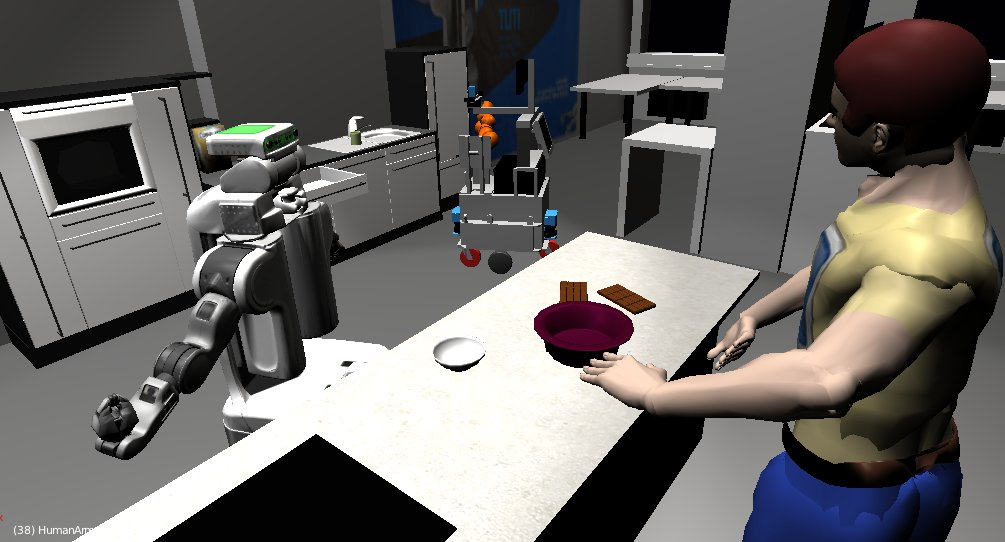
\includegraphics[width=0.9\textwidth]{intro/brownie_scenario.jpg}
	\caption{A representation of the scenario, in the MORSE simulator}
	\label{fig|scenario}
\end{figure*}

In order to illustrate what we consider to be the required features of a
knowledge representation system for robotics, we introduce in this section a
demonstration scenario.

While devising a scenario inevitably constraints the breadth of abilities we
examine, we insist on the fact that our main purpose here is to ground into a
real case the set of representational features we consider as desirable.  We
will \emph{not} evaluate any of the systems we survey in this article by
judging their applicability to this particular scenario.

We entitle our scenario ``the Brownie scenario'' (Fig.~\ref{fig|scenario}).

Robi and Roba are two service robots. They are considered to be able to freely
move and pick objects, but they are not expected to have the exact same
hardware and softwares architectures, and specially, they are not expected to
have the same knowledge representation system. These robots cooperate with a
human in a kitchen environment.

The main task of the scenario is the joint realization of a brownie, initiated
by the human injunction ``Let's make a brownie for tonight!''.

The scenario is successful if the task is achieved (the brownie is baked) and:

\begin{itemize} 

	\item it took less time that it would have require for the human alone, 

	\item it didn't require a heavier cognitive involvement from the human that
	what would have been required without the robots' help.  

\end{itemize}

We voluntarily do not detail the subtasks of the scenario, neither we define
how they are shared amongst agents. In our analysis we focus on the general,
\textit{a priori} representational needs of the scenario.

A ``first-order'' analysis of this task leads to a first partition of the
required representation abilities:

\begin{enumerate}

	\item Representation abilities related to the execution of a complex
	spatio-temporal task,

	\item Representation abilities related to cooperation with other agents.

\end{enumerate}

% Representation of a complex task
We can further refine these categories: to prepare and bake a brownie, the
robot first needs to make sense of the very term \emph{brownie}: what is it?
what is it used for? what is it made of? etc. We call this knowledge
\emph{common-sense knowledge} and the robot must be able not only to represent
it, but also to have some kind of access to it (for instance through a initial
set of facts that are made available at startup, or via access to a Web-based
knowledge base like Wikipedia, etc.)

Bound to the action \emph{make}, this should lead the robot to build and
represent a \emph{context}: we are in a scenario involving cooking. Actions
related to cooking often take place in the kitchen, cooking requires ingredients, 
utensils and a procedure that may be provided by a recipe, etc.

This last sentence implies several other features for our knowledge
representation system: ``cooking often takes place in the kitchen'' implies
that representation of both uncertainty and likelihood is desirable. The fact
that cooking is associated to a place further implies that the system models
locations and is able to attach \emph{thematic relations} to concept
(here, the likely location of the cooking action).

``cooking requires ingredients that may be provided by a recipe'' hints about a
very common feature available in most knowledge representation systems:
\emph{reasoning}. The robot \emph{infers} that cooking may require a recipe
since a list of ingredients is a pre-requisite of the cooking action, and a
recipe may provide such a list. If we omit the ``may'', this is a typical
example of first-order logic reasoning. Many other reasoning techniques exist
(including probabilistic ones -- ones able to deal with the ``may''), we shall
illustrate some of them later in this scenario.

We mentioned that a recipe often provides a procedure (or a \emph{plan}). The robot
should be able to store this plan in a way that allow later execution.  The
plan is likely to contain \emph{spatio-temporal constraints} (like ``put
the brownie in the oven for 20 min'') that must as well be appropriately
represented.

To make decision, a robot may also want to \emph{predict} the state of the world
after some action (``if I leave the cake 2h in the oven, it will be burned'').
Such ability to project itself in future or, generally speaking, in other
possible state of the world is related to several cognitive ability and
reasoning techniques: \emph{planning}, \emph{representation of possible worlds}
and \emph{non-monotonic reasoning}, in addition to common-sense knowledge and
\emph{physics-based reasoning}.

Procedures are in addition often \emph{underspecified}: we can expect the recipe
to provide a cooking duration, but we usually do not expect the recipe to tell
us to first open the oven door, and then put the cake into it, since it is
self-evident that the door must first be opened to put the cake in the oven.
Such underspecification should be detectable, representable, and ideally
completable by the knowledge representation system\footnote{Note that we do not
assume here the {\it knowledge representation system} to be a single software
component: it may well be the result of the aggregation of several modules
working together}.

% Representation feature that enable cooperation
Then, we want our three agents to cooperate. This, in turn, leads to another
set of cognitive abilities.

Cooperation in our scenario can intervene at many places. For instance, an
agent may want to inform another one about the number of eggs that are
necessary for the brownie. This \emph{helping} behaviour makes sense only if
the first agent knows that the recipient agent both needs the information but
does not know it. This in turn requires the robot to be able to model the
knowledge of the other agents: to think \emph{from the perspective} of another
agent (this idea is related to the so-called Theory of Mind~\cite{...}).

Ability to communicate is one important pre-requisite to collaboration.
Communication in general~\cite{Jakobson} requires the addresser and the
addressee to share a common interpretative framework (shared common-sense
knowledge -- or cultural background -- and a shared context). In our scenario,
the agents are working in a kitchen. This element of context does not however
suffice if, for example, an agent asks another agent to ``give {[him]} the
bowl''. Besides the symbol ``bowl'', which physical entity are we actually
talking about? If we want to act on the world, this so-called \emph{grounding}
operation is essential, and may be tightly bound to the underlying knowledge
representation system. Note that grounding usually denotes the {\it top-down}
operation: from the symbol to the percept. It is however commonly bundled with
the converse operation, that retrieve (or create) symbols from perception.

A related ability is called \emph{pre-supposition accomodation}: if one of the
agent moves behind another one, with the brownie dough in its arm, and says
``be careful, I'm behind you!'', we want the first agent to be able to
represent both symbolically and geometrically (because, for instance, if the
agent want to move, it must take into account the new obstacle) something that
was not directly perceived. A knowledge representation system may be able to
provide structures to represent and reason about such cases.

Also central to cooperation are the notions of \emph{joint
intentions} and \emph{joint goals}~\cite{Tomasello2005, Bratman2009}: to help
the human during the cooking session, the robots need to track how far
they are into the recipe, what is the next step the human is likely to go for,
how task are currently split between agents, what action is currently
blocking the procedure, etc. This knowledge should let the robot identify the
intentions of other agents and create accordingly joint goals. Hence, a
knowledge representation system aiming at dealing with cooperative behaviours
is likely to have goal management structures taking explicitly into account
other agents' actions and goals.

In order to effectively share tasks, the robot must also know what it is
capable of: \emph{capability introspection} (both in term of general capability
and of immediate ability) is thus often desirable. More general introspection
(like the ability to tell ``who I am'' or ``what do I think of'' does not
appear to be necessary in our scenario. This may however enrich the human-robot
interaction.

Last but not least, our scenario assumes implicitly \emph{natural interaction}
between humans and robots (as showed by the casual style of the
order ``Let's make a brownie!''). While natural language processing {\it
per-se} is usually out of the scope of a knowledge representation system, we
may want to be sure these systems may successfully interoperate, \ie that the
knowledge representation system provides efficient support to the natural
language processing module (for instance by adopting models and vocabulary that
are both well suited for machine processing and remain as close as possible to
the humans own structures and vocabulary).

%%%%%%%%%%%%%%%%%%%%%%%%%%%%%%%%%%%%%%%%%%%%%%%%%%%%%%%%%%%%%%%%%%%%%%%%%%%%%%%
%%%%%%%%%%%%%%%%%%%%%%%%%%%%%%%%%%%%%%%%%%%%%%%%%%%%%%%%%%%%%%%%%%%%%%%%%%%%%%%
%%%%%%%%%%%%%%%%%%%%%%%%%%%%%%%%%%%%%%%%%%%%%%%%%%%%%%%%%%%%%%%%%%%%%%%%%%%%%%%


\section{Contributions}
\label{sect|contributions}

This section summarizes the main contributions of the thesis, both from a
scientific point of view and from a technical point of view.

\section{Scientific contributions}
\label{sect|scientific-contributions}

The need of a better understanding of the knowledge needs of robotic
applications in human, \ie complex, dynamic, semantically-rich, environments,
is the starting point of this thesis. 

During the preparation of the thesis, the extensive review of the literature,
the formulation of numerous challenging interaction scenarii that led to the
preparation and conduct of several experiments, helped to iteratively refine
the ``knowledge for interaction'' problem. The fundamental scientific outcome
of this work is thus the listing and formal organization of the set of
desirable characteristics of knowledge representation systems for service
robotics, supported by several concrete interaction scenarii.

This typology aims to offer an exhaustive and consistent base to evaluate
existing systems and to draw new research perspectives. It also enables to
better assess the progresses of the Service Robot and Human Robot Interaction
research communities towards the long term goal of \emph{human-level artificial
intelligence} for robots, as would say McCarthy.

Another important scientific contribution of this thesis is to participate to
narrow down the gap between research on embodied and disembodied artificial
agents: we have tried to bridge experiences learned from years of research on
disembodied cognitive architectures (both from the computing science and
neuropsychology communities) with the constraints from real-world systems that
weight on robotic architectures. Notably, we have tried to identify relevant
theoretical references from the diverse fields of cognitive sciences.

At the architectural scale, our work helps to understand the knowledge flows in
modern cognitive architectures for robots. By making knowledge \emph{explicit}
in our architectures, it allows the humans that design and program robots to
\emph{talk about} knowledge: it \emph{materializes} concepts that were
beforehand diffuse and ubiquitous.

This work has also several more focused scientific contributions. The
centralized semantic architecture that we propose is original. While it
exhibits shortcomings for some cognitive tasks, it also offers new efficient
ways to represent and manipulate knowledge. Along with the extensive survey of
current knowledge systems we have conducted, it effectively completes the
panorama of existing designs.

We also have a notable contribution on the grounding of human-robot dialogue in
natural language. We have algorithmically formalized a novel grounding process that
takes advantage of multi-modal communication (verbal, deictic and immanent) and
handles several more complex language features like quantification.

\section{Technical contributions}
\label{sect|technical-contributions}

This thesis has four major technical contributions: the software development of
\emph{ORO server} as a semantic blackboard dedicated to robotics application,
the design of the \emph{ORO ontology} as a domain-specific common-sense
ontology tailored for service robotic needs, the pervasive integration of a new
semantic layer into several existing robot architecture, and finally, the
software development of \emph{Dialogs}, a novel module for natural language
grounding.

\fxwarning{Mention MORSE? How?}

Besides proposing a new integration model for sensor data, natural language and
symbolic knowledge repositories, our work extends these previous contributions
by tackling more realistic human-robot interactions: less restricted speech
understanding; ability to deal with complex, partially unknown human
environments; and fully embodied (with arms, head,...) autonomous robots that
manipulate a large range of household objects.

Three specific contributions are presented in this work: first, we introduce a
versatile and light-weighted knowledge base that models in a formal framework,
based on first-order logics, not only the robot's own beliefs but also every
other cognitive agent the robot interacts with.  This explicit modeling of
other agents' belief states is used for the interaction and eases the
implementation of various advanced cognitive behaviors like
False-Beliefs~\cite{Leslie2000} or interactive object discrimination.

Second, we have implemented a framework to extract symbolic facts from complex
real scenes. It is based on a 3D model of the world that the robot builds
on-line by merging different sensor modalities. It computes spatial relations
between perceived objects in real-time and it allows for virtually \emph{viewing}
of the same scene from different points of view, enabling \emph{visual} and
\emph{spatial agent perspective taking}.

Third, the same symbolic knowledge base enables richer language capabilities
for the robot.  We propose a new approach to natural language grounding that is
robust, situated and more generic than what can be found in previous work
on situated language grounding. We present several examples that include
recognition and semantic validation of thematic roles or disambiguation
based on attention foci.

Communcation between these components is build as streams of symbolic facts,
where knowledge manipulated by the robot is made explicit.
This leads us to the idea of a \emph{knowledge-oriented architecture}, which is
discussed at the end of the article.

These points highlight some original aspects of a larger cognitive architecture
that has been deployed and tested on several mobile robotic platforms
(including both humanoid robots and service robots), demonstrating the
versatility and hardware-agnosticism of these developments.


%%%%%%%%%%%%%%%%%%%%%%%%%%%%%%%%%%%%%%%%%%%%%%%%%%%%%%%%%%%%%%%%%%%%%%%%%%%%%%%
%%%%%%%%%%%%%%%%%%%%%%%%%%%%%%%%%%%%%%%%%%%%%%%%%%%%%%%%%%%%%%%%%%%%%%%%%%%%%%%
%%%%%%%%%%%%%%%%%%%%%%%%%%%%%%%%%%%%%%%%%%%%%%%%%%%%%%%%%%%%%%%%%%%%%%%%%%%%%%%


\section{What are the challenges?}
\label{sect|scenario-challenges}

Those two broad targets should lead to two improvements for human-robot
interaction:


\begin{itemize}
	\item to loosen the constraints on symbolic modelling of the robot
	environment by providing more expressive representation system than
	classical databases or fact repositories,

	\item to improve human-robot interaction by explicitely providing to the
	machine an interpretation frame, at least partially shared with the human.

\end{itemize}


\fxnote{Put focus on knowledge related challenge => focus on questions that need to be
answered}
\fxnote{Show what is difficult in the scenario, and why this requires research.}

\subsection{Specific requirements of human-robot interaction}
\label{sect|pecularities-krs-for-hri}

Pecularities on knowledge representation required by HRI, in the frame of the
general context defined in section~\ref{sect|general-context}:

\subsubsection{Human communication}

\begin{figure}%[!ht]
\centering
  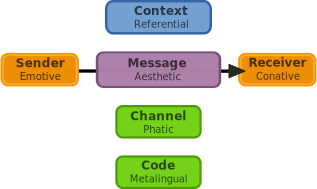
\includegraphics[width=0.6\linewidth]{communication/jakobson_communication_model.pdf}
  \caption{The \emph{Communication Model}, as proposed by Jakobson. In bold
  characters are the \emph{communication dimensions}, in italics, the
  corresponding \emph{communication functions}.}
  \label{fig|jakobson_communication_model}
\end{figure}

\subsubsection{Perspective-Taking, False Beliefs, Theory of Mind}

\fxnote{Present here Sally and Ann}

\subsubsection{and also...}

\begin{itemize}
	\item Ability to talk about concepts that are not immediately perceived by
	the robot


	\item \fxerror{TBD: absence of knowledge representation} Ability to
	represent that an agent knows something about something else, even if we do
	not know \emph{what}.

\end{itemize}

\subsection{Targeted applications/experiments}
\label{sect|targeted-applications-experiments}


The operational targets are two-fold:

\begin{inparaenum}[\itshape a\upshape)]

	\item determine, for a abstract/theoritical/general point of view, how and
	why a cognitive architecture could contribute to these aims; and

	\item implement it.

\end{inparaenum}

\begin{itemize}
	\item \textbf{Categorization}: \emph{Odd One Out}-style experiment,
	\item \textbf{Dialogue}: Grounded dialogue,
	\item \textbf{Introspection verbalization}: Integration dialogue/planing, verbalization of plans,
	\fxerror{TDB: integration dialogue/planing + verbalization of plans}
	\item \textbf{Connection to remote knowledge sources}: \emph{DBpedia}, \emph{WordNet}, \emph{KnowRob ontology}...
	\fxerror{TDB: integration remote knowledge sources}
\end{itemize}

%%%%%%%%%%%%%%%%%%%%%%%%%%%%%%%%%%%%%%%%%%%%%%%%%%%%%%%%%%%%%%%%%%%%%%%%%%%%%%%
%%%%%%%%%%%%%%%%%%%%%%%%%%%%%%%%%%%%%%%%%%%%%%%%%%%%%%%%%%%%%%%%%%%%%%%%%%%%%%%
%%%%%%%%%%%%%%%%%%%%%%%%%%%%%%%%%%%%%%%%%%%%%%%%%%%%%%%%%%%%%%%%%%%%%%%%%%%%%%%


\section{Organisation of the thesis}

\fxnote{Write down the plan}


\chapter{Symbolic Knowledge Representation}
\label{chapt|krs}

\fxnote{Support material: \emph{What is a knowledge representation} by Davis,
Shrobe and Szolovits,
\url{http://groups.csail.mit.edu/medg/ftp/psz/k-rep.html}}

\section{Knowledge and robotics}
\label{sect|knowledge}

The idea of \emph{Cognitive Robotics} was coined in the early 1990s by Reiter.
In a chapter on that subject in \emph{Foundations of Artificial
Intelligence}~\cite{Levesque2008}, Levesque reminds about the manifesto they
wrote together in 1998:

\begin{quotation}

    Central to this effort is to develop an understanding of the relationship
    between the knowledge, the perception, and the action of [\ldots] a robot. The
    sorts of questions we want to be able to answer are

    \begin{itemize} 

        \item to execute a program, what information does a robot need to have
        at the outset versus the information that it can acquire \emph{en route}
        by perceptual means?

        \item what does the robot need to know about its environment versus what
        need only be known by the designer?

        \item when should a robot use perception to find out if something is
        true as opposed to reasoning about what it knows was true in the past?

        \item when should the inner workings of an action be available to the
        robot for reasoning and when should the action be considered primitive
        or atomic?

    \end{itemize}

    and so on. With respect to robotics, our goal (like that of many in AI) is
    \emph{high-level robotic control}: develop a system that is capable of
    generating actions in the world that are appropriate as a function of some
    current set of beliefs and desires.

\end{quotation}

Indeed, pervasive knowledge could safely be considered as the prominent
characteristic of cognitive robotics. This chapter is dedicated to an analysis
of what is knowledge for a robot, and what are the important features of
knowledge and knowledge representation that are relevant to cognitive robotics.

The next section attempts to give a practical definition of knowledge for
robotics, with a few of its major characteristics. We then review some existing
material from diverse fields of cognitive robotics to propose our own
\emph{typology} of the needs and characteristics of knowledge representation
for service and interactive robotics. About fifty such items are identified,
defined, and organised in a large set.

We then put into practice this reference by surveying eight systems and
architectures for robots. Their main strengths are underlined, in order to
depict the state of the research in knowledge representation for robots.

Finally, we conclude this chapter on symbolic knowledge representation by
briefly presenting a novel API for knowledge manipulation, jointly designed
with several other researchers on knowledge representation.

\paragraph{What do we call ``knowledge''?}
\label{sect|on-knowledge}

Since we will discuss at length the concept of knowledge in the context of
robotics in the coming pages, it is useful to make our terminology explicit.

Be it in philosophy, cognitive sciences or computer sciences, reaching an
agreement on a definition of ``knowledge'' seems difficult.

Allen Newell's famous \emph{Knowledge Level}~\cite{Newell1981} can be a
starting point: for Newell, \emph{knowledge} is a medium between \emph{agents}
and \emph{goals}, \emph{actions}, \emph{bodies}. Whereas the symbol level deals
with representation, the knowledge level deals with language, semantics;
whereas the symbol level deals with inference, the knowledge level deals with
entailment. We will, at the conclusion of the thesis, give a second look to
this distinction.

In our robotic context, we define knowledge as a narrower concept, while
keeping Newell's link to actions: ``knowledge'' is for us  \emph{a set of
interrelated logical facts that are meaningful to the robot executive
controller}. By \emph{meaningful} we mean that can possibly be interpreted to
lead to a purposeful action. We will see that our main challenge while
designing a cognitive architecture is furthermore to make this knowledge as
\emph{explicit} as possible.

The relation of \emph{data} and \emph{information} to knowledge is a debated
epistemology question known as the ``DIKW'' hierarchy question. In this thesis,
we will associate data to low-level material like raw sensor output, and
information to uncontextualised symbolic facts.

To give a example, we can imagine a human reading a book while being tracked by
a Kinect sensor: the pose of the human skeleton in the world would be the data,
the fact \concept{looksAt(human, book)} as interpreted by a geometric reasoning
module would be the information, the fact \concept{looksAt(john,
war\_and\_peace)}, fully grounded and connected to the whole knowledge base of
the robot would be proper knowledge.

This simple example also acknowledges the tight coupling between the symbolic
and the geometric realms: while AI at its origins was mostly a matter of
symbolic models, it has been since recognised that not only that the mind is
not a purely abstract system, disconnected from the physical world, but even
more, cognition fundamentally relies on its relation to the physical world
(so-called \emph{embodied cognition}). Varela~\cite{Varela1992} is one of the
main discoverer of these mechanisms, and coined the concept of
\emph{enactivism} as the theoretical framework that study the links between
cognition, embodiment and actions.

From the perspective of communication, knowledge is for us an information
\emph{interpreted in the cultural and social contexts} of the robot. This
translates into three practical features: knowledge is made of statements that
are \emph{contextualized}, \emph{grounded}, and \emph{limited} to a domain of
validity. These three features have important consequences for the way a
knowledge representation and storage system must be designed. Let us examine
them:

\paragraph{Contextualizing} is the ability for a cognitive system to connect a
fact with a \emph{cultural context}, an \emph{interpretive frame} and the set
of other facts previously acquired by the agent.

Since machines are limited to syntactic (in contrast to semantic)
processing, we are mostly looking for a syntactic (\ie, based on symbols)
matching between concepts representations (in our case, sets of alphanumeric
characters).\fxnote{il faut sans doute évoquer ici la relation
sémantique/syntactique que propose Choamsky}.

The \textit{cultural context} is a broad set of common, general facts that are
considered widely accepted among the interactors (\eg ``bottles may contain
water''). This knowledge is often referred as \emph{common-sense knowledge}.

By \emph{interpretive frame} we mean that a concept may have different
interpretations depending on the agent, the current situation or the time frame
the statement belongs to. Since a fact in one frame can be different (or even
inconsistent) with a fact in another frame (for instance, one object can be
visible for the robot and invisible for another agent), the underlying
knowledge representation system must properly handle these interpretive
frames.

Note that effectively representing a context is a rather different task than
identifying it. This aspect will be further discussed at the end of this work.

\paragraph{Grounding} corresponds to the identification or creation, and then,
maintenance of a link between the symbol (the syntactic form of knowledge
the computer will manipulate) and its semantics, \ie its meaning, anchored in
the world (the relations between the symbol, the referent of the symbol, and
mediating minds is classically referred as the \emph{semantic triangle}, and has
been extensively studied in linguistics). The issue of grounding is well known
in cognitive science and is summarised by Harnard~\cite{Harnad1990} by this
question: ``how the semantic interpretation of a formal symbol system can be
made intrinsic to the system?''. This issue has a very practical importance in
robotic: for a robot to be both endowed with a symbolic representational and
reasoning system, and able to \emph{act} in the physical world, it must ground
its knowledge.

\paragraph{Domain of validity} specifies the scope in which
an information is (believed to be) true. It covers several aspects: temporal,
situational and probabilistic. While related to the previous concept of
\emph{interpretive frames}, the domain of validity addresses the question
whether a fact must be or not considered in a given context. This validity
limitation is not usually carried by the fact itself. In the previous example,
for instance, the robot observes a human sitting at a table.  The fact ``a
human is sitting at the table'' is true only for a limited period of time,
until the human stands up. This period of time is not directly accessible
(the robot does not know how long the human plans to stay), but the
knowledge representation must be able to deal with this uncertainty and
should explicitly label this fact as being limited in time.

To know if a fact is \emph{permanent} or \emph{transitional} (Pollock
\cite{Pollock1998}, page 51) is difficult (especially considering that a
feature may be considered as permanent or not depending of the context: within
the situation ``a family meal'', the fact ``the human is sitting at the
table'' could be considered as permanent. Conversely, ``ground is static'' is
generally considered as a permanent fact, expect if we are talking of planetary
mechanics for instance. The difficulty lies in the selection of the relevant
situation in which reasoning must be carried out at a given time) and have
currently to be defined in the cultural background of the robot.

These three aspects lead us to envisage the question of knowledge
representation from two perspectives: elements that are \emph{essential} to the
knowledge (without those, informations could not become knowledge), and
processes that are necessary to \emph{produce} knowledge.

Knowledge is essentially dependent on the ability to represent:

\begin{itemize}

    \item links, connections between atoms of knowledge,

    \item a general cultural background, in the form of common-sense knowledge,

    \item interpretive frames, contexts, restrictions on the domain of
    validity.

\end{itemize}

It must also rely the following active processes to:

\begin{itemize}

    \item acquire and maintain knowledge perceived from the physical world or
        retrieved from other sources (interaction with other agents, web-based
        contents,...)

    \item add and connect new facts to existing ones,

    \item monitor contexts and accordingly manage the validity of the stored
        knowledge,

    \item ensure the logical consistency of the knowledge repository, and
    explicit inconsistencies when required\footnote{One may argue that the
    real world is however inherently inconsistent; we will discuss several
    aspects of inconsistencies representation and management later on.}.

\end{itemize}

We have already seen in the imaginary scenario introduced in
chapter~\ref{chapt|introduction} that many other cognitive abilities related to
knowledge representation and manipulation are required by service robots to
actually operate, and the above items are more a high-level view of what
knowledge \emph{intrinsically} need to exist. The next section aims at
providing a large, comprehensive set of cognitive abilities related to
knowledge, that encompasses both essential and non-essential features of
knowledge representation systems.


%%%%%%%%%%%%%%%%%%%%%%%%%%%%%%%%%%%%%%%%%%%%%%%%%%%%%%%%%%%%%%%%%%%%%%%%%%%%%%%%%%%%%%%%%%%
%%%%%%%%%%%%%%%%%%%%%%%%%%%%%%%%%%%%%%%%%%%%%%%%%%%%%%%%%%%%%%%%%%%%%%%%%%%%%%%%
\section{A typology of knowledge representation requirements for robotics}
\label{sect|features}

This section now focuses on formalizing the knowledge representation issue: we
aim first at establishing a comprehensive typology and nomenclature
(figure~\ref{fig|taxo}) of representational needs for robotics in the specific
context of service robotics, before painting, at
section~\ref{sect|surveyed-systems}, the current landscape of approaches to the
knowledge representation problem in the research community. For each such
``dimensions'' of knowledge representation system, we provide a short
definition accompanied by links to relevant literature.

\begin{figure}
        \centering
        \includegraphics[width=1\columnwidth]{taxonomy.pdf}
        \caption{Taxonomy of the analysis dimensions of knowledge
        representation systems for service robotics.}
        \label{fig|taxo}
\end{figure}

The typology has been built from three main sources: a review of the existing
literature on that topic that we present in the next section; the survey of
eight knowledge representation systems already deployed; our own experience,
acquired during the thesis preparation with the help of many discussions with
researchers from both CNRS and TUM, that allowed to interweave two slightly
different perspectives on knowledge in robotics.

We also wish to mention that the short presentation of each feature does not
claim to be a comprehensive summary of the field: it is beyond our capabilities
to cover in a few lines all what the areas of \emph{time representation},
\emph{planing} or \emph{formal logic} have said during the last 30 years. We
indeed focus on the aspects relevant to knowledge representation and certainly
involuntarily omit many significant works in these fields.

\subsection{Previous work}
\label{sect|evaluation-literature}

As said, the typology we propose is in part based on a comprehensive synthesis of
classifications and analysis found in the literature. This synthesis is focused
on cognitive abilities strictly related to knowledge manipulation in the
context of service robotics.

Levesque and Lakemeyer~\cite{Levesque2008} present in their chapter on
Cognitive Robotics several characteristics of knowledge representation systems
for robots, stressing the need of representing the \emph{dynamics of the
world}.  Sensing is included in the knowledge representation via
\emph{fluents}; they introduce the idea of \emph{possible worlds} to represent
distinct parallel mental models; action representation and reasoning about
tasks is discussed in the context of \emph{situation calculus}; \emph{open
world} vs. \emph{closed world} approaches are mentioned.  They also discuss how
robot programming and knowledge representation can be related. We integrate
most of these items in our typology.

In a slightly broader context, Heintz et al.~\cite{Heintz2008} define
\emph{knowledge processing middleware} as systems supporting ``declarative
specifications for flexible configuration and dynamic reconfiguration of
context dependent processing at many different levels of abstraction''. They
identify six characteristics: the system must be able to \emph{merge
informations} from different, possibly distributed sources; it should support
quantitative as well as qualitative processing of information, it should offer
\emph{bottom-up} and \emph{top-down} processing, it should be able to deal with
\emph{uncertainty}, allow for ``flexible configuration and reconfiguration''
(which require what we call here \emph{non-monotonicity}) and finally
\emph{meta-knowledge} and \emph{introspective capacities} (``declarative
specification of the processing functionalities'').

Several surveys compare global cognitive architectures \cite{Langley2006,
Vernon2007, Chong2009}. Langley, Laird and Rogers~\cite{Langley2006}
distinguish nine capabilities: recognition and categorisation, decision making,
perception and situation assessment, prediction and monitoring, planning,
reasoning, execution control, interaction and
learning/remembering/introspection. They also separately identify four
\emph{properties} of a cognitive architecture, that categorise how knowledge is
handled by the architecture: representation of knowledge, organisation of
knowledge, utilisation of knowledge and acquisition and refinement of
knowledge. This categorisation had a notable influence on our typology, and
many of these categories are also present in our proposal.

Vernon et al.~\cite{Vernon2007} split these architectures into two broad
categories: the \emph{cognitivist} ones (where cognition is considered as an
explicit computation problem, often based on symbol manipulation), and the
\emph{emergent} ones (where cognition only exists as a result of the
interaction of the system with its environment). The approaches presented in
this chapter are, at a few exceptions, prototypical \emph{cognitivist} approaches
that aim at making knowledge explicit within the robot architecture. Vernon et
al. propose twelve \emph{characteristics of cognitive system} to compare
architectures. Amongst them, they mention the \emph{inter-agent epistemology}
(how the structure of the world is captured in a representation and shared),
the relation to \emph{embodiment}, the ability to \emph{anticipate} and to
\emph{adapt}, and the mechanisms of \emph{motivation}. While presented at the
level of the whole robotic architecture, these features also translate into
knowledge representation strategies and are relevant to our study.

Chong et al.~\cite{Chong2009} also provide a recent review of the main cognitive
architectures, with a focus on eight functions: perception, memory, goals
management, problem solving capabilities, planning, reasoning, learning and
links to neurobiology.

At an even broader scope, several authors from fields that are connected to
robotics have previously listed desirable features of artificial systems aiming
at rich cognitive abilities.

For instance McCarthy recently listed in~\cite{McCarthy2007} the challenges he
identifies on the road to a \emph{human-level AI}.

\begin{itemize}

	\item the ability to \emph{"operate successfully in the common sense
	informatic situation"},

	\item the necessity of relying on mathematical logic, as the most fruitful
	formalism for machine intelligence,

	\item the ability to deal with \emph{approximate concepts and approximate
	theories} (that would include representing them, and reasoning with them),

	\item non-monotonic reasoning,

	\item what McCarthy calls \emph{Elaboration Tolerance}: the ability to
	extend \emph{on demand} the closed domain of interpretation for a
	given assertion,

	\item the ability to formalise and reason about contexts,

	\item reasoning about events, and in particular, actions,

	\item the capacity of introspection,

	\item and finally, he points the issue of giving computer the right
	heuristics for decision making.

\end{itemize}

Coming from the perspective of natural language processing in situated context,
Roy and Reiter summarise in~\cite{Roy2005} what they see as the main challenges
to be tackled by knowledge representation systems: \emph{cross-modal
representation} systems, association of words with perceptual and action
categories (\emph{grounding}), modeling of \emph{context}, definition of the
right \emph{granularity} of models, integration of \emph{temporal modeling and
planning}, ability to \emph{match past (learned) experiences} with the current
interaction and ability to take into account the \emph{human perspective}.

Knowledge representation systems in robotics are directly affected by these
points, and we indeed integrate them in our typology, in slightly reformulated
ways.


\subsection{What can be represented?}
\label{sect|expressiveness}

\begin{scriptsize}
\begin{center}
\begin{tikzpicture}[taxonomy]
    \node [taxon] {\bf A. Expressiveness}
            child {node [taxon] {{\bf A.5}. Meta-cognition}}
            child {node [taxon] {{\bf A.4}. Uncertainty}}
            child {node [taxon] {{\bf A.3}. OWA/CWA}}
            child {node [taxon] {{\bf A.2}. Expressive power}}
            child {node [taxon] {{\bf A.1}. Logic formalism}};
\end{tikzpicture}
\end{center}
\end{scriptsize}

This first axis of analysis is its intrinsic expressive power. It answers the
question: what can be possibly represented. When it explicitly exists, the
\emph{language} of representation plays here an obvious role.

\subsubsection{Main logic formalisms}

The main role of a knowledge representation system is to provide an adequate
representation system to formally store facts and concepts that could be informally
described in natural language.

Formal logic aims at providing such a representation system with the added
value of providing a tractable support for inference and reasoning.

Most (but not all) of the systems we have surveyed rely on a particular logic
formalism. The choice of the formalism has a strong impact, on one side, on the
range of ideas that can be expressed conveniently (\emph{practical
expressiveness}) or at all (\emph{theoretical expressiveness}), on the other
side, on the ability to solve the fundamental inference problem (called
\emph{satisfiability}: is a given logical sentence true in my model?) in a
tractable manner.

A large number of logic formalisms do exist and we briefly present below the most
relevant ones for systems actually deployed in robotic architectures.

\emph{Predicate logic} is the family of logic formalisms the most commonly
found in knowledge representation. It distinguishes itself from the simpler
\emph{propositional logic} by the use of quantification to increase generality.
\emph{First-order logic} (FOL) is the subpart of \emph{predicate logic} where the
objects of \emph{predicates} (or \emph{formulae}) are simple \emph{terms},
while in \emph{higher-order logics}, predicates can be themselves objects of
other predicates.

\emph{Horn clauses} are an important subset of FOL because the satisfiability
of a set of such clauses is a $P$-complete problem (\ie practically tractable).
A Horn clause is a disjunction of literals (a \emph{clause}) with at most one
positive literal: $\neg p \lor \neg q \lor \cdots \lor \neg t \lor u$, which
can also be represented as $(p \land q \land \cdots \land t) \rightarrow u$.
Important logic programming languages like Prolog are based on Horn clauses.

The family of \emph{Description Logics}~\cite{Baader2008} also plays an
important role. It is also a subset of the first-order logic, with some
extensions in second-order logic. Description logics are notable because most
of them are known to be decidable (but not always in a practically tractable
manner). In description logic, axioms are build from \emph{concepts},
\emph{roles} (that are unary or binary predicates) and \emph{individuals}. The
W3C OWL-DL standard is a widely-used language to describe domains with the
description logic.

Because description logics have been originally created from the perspective of
a \emph{knowledge representation language} and not a logic language, their
terminology (\emph{concept} or \emph{class}, \emph{role} or \emph{property},
\emph{individual},\ldots) is well-suited to knowledge description.

\emph{Modal logic}, that allows for statement qualification like
\emph{possibility} or \emph{necessity}, have been shown to be closely related
to description logics~\cite{Baader2001}. Modal logic allows to represent conveniently parallel
possible worlds and facts like ``the robot knows \emph{that the human knows}
how to read a recipe''.

\fxwarning{On modal logics, see the remark of McCarthy, in \cite{McCarthy2007}, section 3}

\emph{Temporal logic} are designed to represent and manipulate assertions whose
truth value may vary in time. We introduce one of its key idea (the
\emph{fluents}) later in the typology.

One last class of logics that is of particular relevance for robotic
applications is the \emph{probabilistic logics} or \emph{Bayesian logics}.
These logics provide a formal framework to reason on propositions whose truth
or falsity is uncertain. We elaborate below on the representation of uncertainty.

Note that most of these logic formalisms are still active research field on
their own, and practical considerations (especially the availability of
reasoners efficient enough for on-line use on a robot) often constrain the
choice of a logical formalism and a level of expressive power.

\subsubsection{Expressive power}

Logical formalisms each bring a certain level of expressive power. For
instance, the following classical syllogism can not be represented in
propositional logic because of the use of \emph{universal quantification}:

\begin{quote}
\begin{enumerate}
    \item All men are mortal,
    \item Socrates is a man,
    \item Therefore, Socrates is mortal
\end{enumerate}
\end{quote}

However, the following weak version of the syllogism can be represented in
propositional logic:

\begin{quote}
\begin{enumerate}
    \item If Socrates is a man, then Socrates is mortal,
    \item Socrates is a man,
    \item Therefore, Socrates is mortal
\end{enumerate}
\end{quote}

Generally speaking, expressive power comes at the cost of more complex
\emph{satisfiability} and \emph{consistency}\footnote{We precise these concepts
at section~\ref{sect|reasoning}.} computations, possibly leading to
untractable, if not undecidable (\ie systems where it is proven that a
proposition can not be decided to be true or false) problems.

\begin{figure}
    \centering
    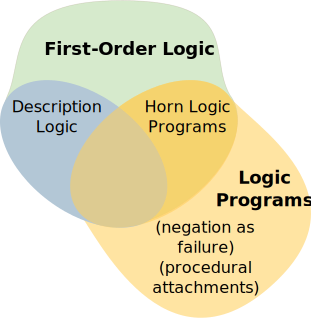
\includegraphics[width=0.3\columnwidth]{typology/expressive_overlap_dl_horn.pdf}
    \caption{expressiveness overlap of Description Logics and logic programs
    based on Horn clauses, taken from~\cite{Grosof2003}}
    \label{fig|overlap_dl_horn}
\end{figure}

Figure~\ref{fig|overlap_dl_horn} shows that the expressive power of description
logics and Horn clauses partially overlaps. In section~\ref{sect|reasoning} we
mention extensions to description logics based on rule systems that bring closer
the two approaches.

The relationships between expressive power and reasoning complexity that follow
has been extensively studied for Description Logics.
Zolin~\cite{ZolinDLComplexityNavigator} maintains a ``complexity navigator''
that allows to conveniently explore these relationships and indexes most of the
literature on that subject.

It can be noted that the relation between expressiveness and reasoning
complexity is fragile: for instance, adding the following axiom \stmt{farFrom
disjointProperty near} (that states that two individuals can not be at the same
time near and far from each other) changes the expressiveness power of the ORO
Common-Sense ontology (presented at chapter~\ref{chapt|oroserver}) from
$\mathcal{SHOIQ(D)}$ to $\mathcal{SROIQ(D)}$\footnote{See
appendix~\ref{chapt|dl} for a brief explanation of this notation}: this
seemingly innocuous assertion change the complexity class of the whole
ontology, and the concept satisfiability reasoning problem switches from a {\it
NExpTime-complete} problem to a {\it NExpTime-hard} problem (\ie, \emph{at
least} as hard as the hardest problem in {\it NExpTime}).

This ``instability'' has practical consequences on run-time performances on
the robot because a light alteration of the knowledge structure can lead to
very noticeable performance drops.


\subsubsection{Open world and close world assumptions}
\label{sect|owa-cwa}

The \emph{close world} (CWA) vs. \emph{open world} (OWA) assumptions name a
modelling choice on the \emph{completeness} of a knowledge domain. In the close
world assumption, a proposition that can not be proven true is assumed to be
false (\emph{negation by failure}), while in the open world assumption, a
proposition may be considered either true, false or unknown.

This distinction is important in robotics where the robot may have to manipulate
concepts with only partial knowledge on them. For instance, let us imagine a robot
that sees a bottle on a table, whose bottom is hidden by another object. The
robot can not prove that the bottle is indeed \emph{on} the table. A knowledge
representation system relying on the closed world assumption would then assume
the bottle is \emph{not} on the table ($\lnot R^{CWA}_{isOn}(bottle, table)$)
whereas with the open world assumption, the proposition $R^{OWA}_{isOn}(bottle,
table)$ would be undecided. Example in table~\ref{table|cwa-owa-example} provides
another example of consequences of the CWA/OWA choice on reasoning.

\begin{table}
    \begin{center}
    \begin{tabular}{ll}
    {\bf Action} & {\bf Part involved} \\
    \hline
    {\tt PickSoftly} & hand \\
    {\tt PickAndPlace} & arm, hand \\
    {\tt MoveArm} & arm \\
    \hline
    \end{tabular}
    \end{center}
    \caption{Assuming the question is: \emph{select actions that do not require
    to move the arm}, a CWA reasoner would return {\tt PickSoftly} whereas an
    OWA reasoner would not return anything if the {\tt PickSoftly} action is
    not explicitly said not to involve the arm.}
    \label{table|cwa-owa-example}
\end{table}

The OWL language is specifically known to assume an open world.  Domains
constrained with the closed world assumption lead to more tractable inference
problems, and allow for instance the use of logic languages like Prolog. Thus,
several approaches exists to \emph{locally close} a domain (\cf
Levesque~\cite{Levesque2008}, section 24.3.2 for a summary of those ones).

\subsubsection{Representation of uncertainty and likelihood}

Sources of uncertainty for a robot are two-fold: uncertainty \emph{intrinsic}
to facts (like \emph{``It may rain tomorrow''}), uncertainty caused by
imperfect perception of the world (\emph{``Is the bottle really on the
table?''}). Most logics do not account explicitly for uncertainty. It must be
either relied on specific logics (like Bayesian logics) or on extensions of
classical logics.

%\fxfatal{Representation of uncertainty: To be completed!}

\subsubsection{Meta-cognition: knowledge on the knowledge}

As stated by Cox and Raja~\cite{Cox2007}, meta-cognition is composed of both
\emph{``meta-level control of cognitive activities and the introspective
monitoring of such activities to evaluate and to explain them"}.

Sloman proposes in~\cite{Sloman2011} a detailed analysis of meta-cognition and
its different aspects in both natural (human) and artificial systems.

A knowledge representation system endowed with \emph{meta-cognition} is not
only able to manipulate knowledge but also to exhibit and manipulate the
structure of its knowledge and the reasoning process. For instance, the ability
to explain a logical inconsistency in a KRS is a meta-cognitive function, as is
the ability to expose and alter the knowledge structure (these two reasoning
techniques have their own entries in the taxonomy, at
section~\ref{sect|reasoning}.

At section~\ref{sect|introspection} below, we discuss the idea of
introspection.  Meta-cognition can be viewed as the technical facet of the
introspection in general.


%%%%%%%%%%
\subsection{How things are represented?}
\label{sect|higher-level-domain-representation}

We do not discuss in this section the general strategies to construct a
knowledge model (they will be presented in
section~\ref{sect|design-strategies}). We focus here on questions that involve
representational challenges (time, space, context) or require specific
cognitive capabilities (theory of mind, introspection, memory).

\begin{scriptsize}
\begin{center}
\begin{tikzpicture}[taxonomy]
    \node [taxon] {\bf B. Representation}
            child {node [taxon] {{\bf B.5}. Memory}}
            child {node [taxon] {{\bf B.4}. Introspection}}
            child {node [taxon] {{\bf B.3}. Modality}}
            child {node [taxon] {{\bf B.2}. Context}}
            child {node [taxon] {{\bf B.1}. Roles}};
\end{tikzpicture}
\end{center}
\end{scriptsize}

\subsubsection{Role representations}

This section discusses strategies and approaches to represent in a knowledge
model three important \emph{roles}: spatial relations, time and representation
of actions.

\begin{scriptsize}
\begin{center}
\begin{tikzpicture}[taxonomy]
    \node [taxon] {\bf B.1 Roles}
            child {node [taxon] {{\bf B.1.3}. Actions}}
            child {node [taxon] {{\bf B.1.2}. Time}}
            child {node [taxon] {{\bf B.1.1}. Space}};
\end{tikzpicture}
\end{center}
\end{scriptsize}


\paragraph{Representation of space}

Symbolic representation of space is a widely studied topic. In particular, a
large literature corpus is available on spatial ontologies\fxwarning{Which one?}.

Two main classes of spatial relations are usually represented at the symbolic
level: the topology of environments and the placement of physical entities.

\begin{scriptsize}
\begin{center}
\begin{tikzpicture}[taxonomy]
    \node [taxon] {\bf B.1.1 Space}
            child {node [taxon] {{\bf B.1.1.2}. Placement}}
            child {node [taxon] {{\bf B.1.1.1}. Topology}};
\end{tikzpicture}
\end{center}
\end{scriptsize}

Topological maps are abstractions of an environment as graphs where nodes
represent places and edges represent connections between places. Because they
are symbolic representation, topological maps allow higher-level reasoning
(such as containment, connectivity, regions) than metric maps.

One important contribution to the building of a coherent representational stack
for space representation is the Spatial Semantic Hierarchy~\cite{Kuipers2000}
introduced by Kuipers. It consists in multiple interacting representations of
space, both qualitative and quantitative, that span from sensor-level
representation to ontologies of places and regions.

Symbolic representation of entities placement can be absolute or relative. The
relation \concept{isOn}, for example, leads to absolute statements: the
validity of the relation is independent of the nature of its subjects and
objects, and is also independent of the observer.

On the contrary, the relation \concept{nextTo} is relative, and depends on the
relative size of the subject and the object. Two houses distant of 2 meters
from each other can be considered as next to each other. Two ants separated by
2 meters are not next to each other.

The relation \concept{leftOf} is another example of relative spatial relation,
this time because it depends on the observer viewpoint.

\fxwarning{\concept{front}/\concept{back} -> entities have or not a concept of front/back.}

Choices must be made in the knowledge representation system to adequately
represent relative spatial relations. Options include the computation of such
relations only on-demand, when the context is known (which viewpoints, etc.) or
storage of these facts in different models, one per agent.

\fxwarning{Find references on that subject -> classification of spatial
relations. Wikipedia?}

\paragraph{Representation of time}
\label{sect|time-representation}

As an agent acting at human-like time scale and dealing with temporal concepts
(like actions), a robot needs to represent and reason about
time. Time representation is split into two distinct abilities: representing
time points (both in the past -- which is roughly equivalent to assignment of
timestamps to events the robot perceives -- and in the future), and
representing passing time (situations, durations, timespans) like in
\emph{``the eggs will be cooked in 10 min''}.

This is usually formalised as a disjunction in time representation between
\emph{events}, that is, any durationless temporal concept, and
\emph{situations}, that is, any temporal concept with a non-zero
duration\footnote{Other definitions of a situation do exist, notably in the
context of \emph{situation calculus}~\cite{Levesque1998}, Reiter and Levesque
consider a situation to be an history of actions.}.

Numerous techniques to represent and reason about time have been devised.
Amongst the most significant ones, we can mention Allen's interval
algebra~\cite{Allen1984} and Ghallab's chronicles~\cite{Ghallab1996}.
\fxwarning{We could detail more chronicles and allen algebra...}
The concept of \emph{fluent} also play an important role for time
representation: fluents are properties (or \emph{conditions}) that change over
time, like $sees(agent1, apple, t)$.\fxwarning{A bit short... citation?}

We call a system that does not account for time (\ie that mentally permanently
lives in present) \emph{atemporal}.


\paragraph{Actions}

Events and actions are two temporal concepts that are of particular importance to
robotic systems, as systems that perceive, react and perform in their environment.

While representation of events boils down to label a timestamp, representation
of actions are more complex since not only they deal with durations, but they
also imply semantic interactions between concepts. From a taxonomy point of
view, actions are a particular type of event that normally leads to a situation
corresponding to the action realisation.


\emph{Thematic roles}~\cite{Gruber1965} (also found as \emph{semantic roles} or
\emph{theta roles} in the literature) allow to semantically qualify the
parameters of an action. The recipient of the action, the performer, the object
acted upon, the destination are some example of common thematic roles.
Table~\ref{table|theta-roles} presents a more comprehensive list of thematic
roles proposed by \cite{Aarts1997} (see~\cite{Gutierrez2001} for a comparison
of other sets of thematic roles present in the literature).

\begin{table}
\begin{center}

\begin{tabular}{lp{12cm}}

\toprule
       Role & Meaning \\
\midrule
      Agent & The \emph{doer} or instigator of the action denoted by the predicate. \\
    Patient & The \emph{undergoer} of the action or event denoted by the predicate. \\
      Theme & The entity that is moved by the action or event denoted by the predicate. \\
Experiencer & The living entity that experiences the action or event denoted by the predicate. \\
       Goal & The location or entity in the direction of which something moves. \\
Benefactive & The entity that benefits from the action or event denoted by the predicate. \\
     Source & The location or entity from which something moves. \\
 Instrument & The medium by which the action or event denoted by the predicate is carried out. \\
   Locative & The specification of the place where the action or event denoted by the predicate in situated. \\
\bottomrule

\end{tabular}
\end{center}

\caption{A list of thematic roles, as proposed by Aarts~\cite{Aarts1997}.
Depending on the action, only certain roles are meaningful.}

\label{table|theta-roles}
\end{table}

In the context of robotic, \emph{task} often represents an aggregate of
(atomic) actions. We use the term here as the representation of the abstract
model of an action. Tasks usually specify at least the conditions required to
performed the action and the consequences of the realization of the action, and
are central to the decisional layers of the robot, in particular for the
planning, monitoring and execution control activities. Knowledge representation
systems may thus have specific mechanisms to represent them (and possible, to
reason about them, as presented in section~\ref{sect|planning}).

An technical report we have written on task modeling in OWL ontologies is
available in appendix \ref{appendix|tasks}.

Plans representation is closely related to action and task representation. It
is specifically discussed at section~\ref{sect|planning}.

\subsubsection{Context modeling}

Knowledge is contextualized information: it is essential for the robot to
associate the facts it represents to a \emph{context}. The context carries the
keys for the interpretation of the information and set a common ground for
interaction (and, in particular, communication~\cite{Jakobson1960}). It
implicitely defines the domain of validity of the facts and carries the
\emph{common-sense} knowledge required to fill the gaps of the knowledge
explicitely shared between the agents.

Context is generally difficult to recognise, represent and reuse because it is
multiform and largely implicit nature. It is also never unique: at a given
moment, several contexts, at different temporal, spatial, social scales,
overlap.

In the current literature in robotics and cognitive architectures, the term
\emph{context} usually simply refers to a set of beliefs that initiate a
representation (and reasoning) frame: in~\cite{Lemaignan2011a}, the robot
creates a context of interaction with a specific human by storing in a separate
model the beliefs of this human and using this knowledge when dialoging with
the human, the reasoning network is reinitialised in the GLAIR architecture
when the hypotheses that defined the current situation are not believed
anymore~\cite{Shapiro2009}.

This acception of \emph{context} is simplistic, and omit the overlapping and
multi-scale aspects of context modeling.

We see context representation as one of the main challenge of knowledge
representatio in general, and we will further discuss the importance and issues
brought by context modeling in the conclusion of the thesis.

\subsubsection{Modality, contingency and theory of mind}
\label{sect|possible-worlds}

Linked to the context representation, but seen from another angle, knowledge
representation systems may support logical \emph{modality}. A knowledge model
is logically modal if is support the concept of \emph{possible worlds}, \ie,
parallel beliefs models (or \emph{interpretations}) that can be independently
accessed.

A \emph{contingent} proposition is defined as neither always true (a tautology)
nor always false (a contradiction) in every possible world: its truth value
depends on the context. In knowledge representation systems for robotics that
support logical modality, interpretations are often initialised with a common
set of initial beliefs (like common-sense knowledge). This initial common
knowledge is hence true in every possible worlds for the robot, and thus does
not belong to its contingent knowledge.

On the contrary, alternative mental models with contingent knowledge may be
used to represent different (possibly hypothetical or even imaginary) views on
the world, from the robot own perspective or context, or from other
perspectives computed by the robot.

The representation of the mental perspective of other agents has a particular
importance in human-robot interaction. It relies first on the ability to
literally \emph{view} the world from a standpoint which is not
\emph{egocentric}. This cognitive ability is referred as \emph{perspective
taking}. Flavell~\cite{Flavell1992} and Tversky~\cite{Tversky1999} define the
psychological grounds of perspective taking, that are themself originated in
Piaget's work on cognitive development (recent studies on infants include
Moll~\cite{Moll2006} for instance). Perspective taking begins to be studied on
robots as well~\cite{Trafton2005, Breazeal2006, Ros2010}.

The idea of a \emph{theory of mind}~\cite{Premack1978} emerges from the
perspective taking ability. It can be defined as the ability for one to
understand and acknowledge that other intelligent agents can have their own
mental state (that includes beliefs, intents, desires, knowledge) that is
possibly different from one's own. The \emph{attention} plays a central to the
development and recognition of a theory of mind~\cite{Baron-Cohen1985,
Leslie2000}.

A notable consequence of having a theory of mind is the representation of
\emph{false beliefs}, \ie, facts that are believed to be true for an agent, but
false for other ones. The \emph{Sally and Ann} experiment~\cite{Leslie2000}
(figure~\ref{fig|sally-ann}) is a classical example of a false belief
situation. In~\ref{fig|sally-ann-final}, Sally thinks the ball is in the beige
box because she did not see Ann moving it. An external observer asked ``Where
will Sally look for the ball?'' would answer ``in the blue box'' without a
theory of mind (\ie, a model of the knowledge of Sally), whereas it would
correctly answer ``In the beige box'' with a theory of mind.

\begin{figure}
        \centering
        \subfigure[Sally puts the ball in the beige box.]{
            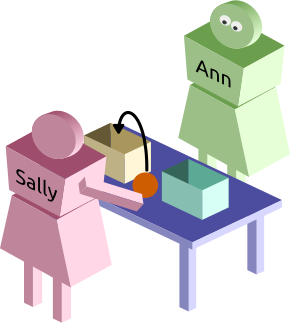
\includegraphics[scale=0.4]{typology/sally_ann1.pdf}
        } \hspace{15pt} %
        \subfigure[Sally goes away.]{
            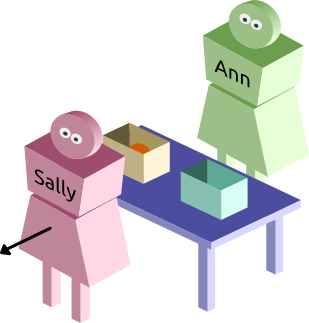
\includegraphics[scale=0.4]{typology/sally_ann2.pdf}
        } \\
        \subfigure[Ann moves the ball.]{
            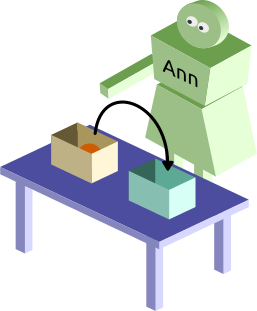
\includegraphics[scale=0.4]{typology/sally_ann3.pdf}
        } \hspace{15pt} %
        \subfigure[Where will Sally look for the ball?]{
            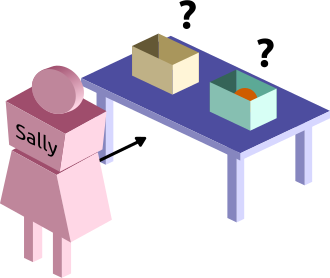
\includegraphics[scale=0.4]{typology/sally_ann4.pdf}
            \label{fig|sally-ann-final}
        }
        \caption{The standard ``Sally and Ann'' false-beliefs experiment, taken
        from~\cite{Leslie2000}.}

        \label{fig|sally-ann}
\end{figure}

Scassellati~\cite{Scassellati2002} is one of the first to have implemented a
theory of mind on a humanoid robot.



\subsubsection{Self-knowledge: Who am I? What can I do?}
\label{sect|introspection}

\paragraph{Self-knowledge}

\emph{Self-knowledge} is the term used in philosophy and psychology to describe
the knowledge that an individual has, acquires or infers about itself through
its experiences. It answers the question ``What am I like?''.

Introspection is the technical meaning to access to self-knowledge by the
ability to self describe: what are my capabilities, what is my state
(performing some action, idling, etc.), what are my beliefs, what are my
intentions and my plans?

Introspection must be distinguished from meta-cognition: While introspection
may require meta-cognition (for instance to be able to expose its internal
knowledge), it is not always mandatory. The current state of the robot can be
represented as a simple instantiation of a specific category (for instance, if
the robot gives an object to the human, this state could be represented with the
triples \setstmt{robot performs action1,action1 isA Give}.

\paragraph{Modeling of the robot capabilities}

A particularly important aspect of self-knowledge for robots relates to the
description of its own capabilities: which sensors/actuators/computation
services exist and are currently available ?  While at a first level, these
descriptions can be static (\eg the robot has one laser scanner and two arms),
at more advanced levels, the description is updated and reflect the current
(and possibly past and future) state of the robot. Note that these descriptions
may also involve geometric descriptions (a kinematic chain, the pose of a
device, etc.) that may be deported outside of the main knowledge base. Efforts
trying to formalize, maintain and expose the capabilities and state of a robot
are not new (and ground themselves in work and techniques for self-descriptive
remote procedure calls in computing science), but take a renewed importance
with applications for high-level multi-robot cooperation.

Recent works by Kunze et al.~\cite{Kunze2011} seeks at defining a formal
language to represent the capabilities of a robot.

\subsubsection{Memory}
\label{sect|memory}

Memory has been studied at length in the cognitive psychology and
neuropsychology communities: Atkinson and Shiffrin~\cite{Atkinson1968}
introduce the idea of \emph{short-term} and \emph{long-term} memory,
Anderson~\cite{Anderson1976} splits memory into \emph{declarative} (explicit)
and \emph{procedural} (implicit) memories, Tulving~\cite{Tulving1985} organises
the concepts of \emph{procedural}, \emph{semantic} and \emph{episodic} memories
into a hierarchy. Short-term memory is refined with the concept of
\emph{working memory} by Baddeley~\cite{Baddeley2010}
(Figure~\ref{fig|memory_models}).

\begin{figure}
    \centering
    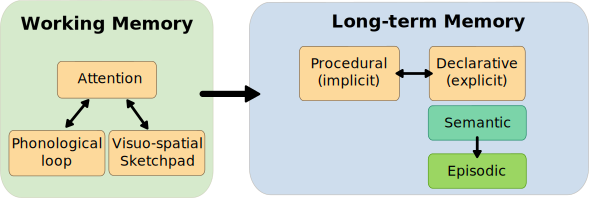
\includegraphics[width=0.6\columnwidth]{typology/memory_models.pdf}

    \caption{Overview of the main types of memories, based
    on~\cite{Atkinson1968, Anderson1976, Tulving1985, Baddeley2010}}

    \label{fig|memory_models}
\end{figure}

It is worth emphasising that if memory is commonly associated to the process of
forgetting facts after a variable amount of \emph{time}, it actually covers
more mechanisms that are relevant to robotics, like selective remembering
triggered by a specific context or reinforcement learning.

Most knowledge representation systems offers some kind of memory as a pool of
facts that are not forgotten by the robot until it is halted (this memory is
often referred as a \emph{working memory}, but with a meaning unrelated to
Baddeley's definition). Some systems may propose persistent storages that allow
the robot knowledge to grow over time, while others may offer a larger range of
memory categories, like short term memory (that lasts for a couple of seconds)
or episodic memory (that allows the robot to selectively remember facts
associated to specific events).

In the larger field of cognitive architectures, the {\sc Soar}
architecture~\cite{Lehman2006} is one of those that tries to reproduce a
human-like memory organisation. The GLAIR cognitive architecture also have a
concept of long term/short term and episodic/semantic memories.

%%%%%%%%%%
\subsection{Reasoning techniques}
\label{sect|reasoning}

\begin{scriptsize}
\begin{center}
\begin{tikzpicture}[taxonomy]
    \node [taxon] {\bf C. Reasoning}
%            child {node [taxon] {{\bf C.10}. Learning}}
            child {node [taxon] {{\bf C.9}. Naive physics}}
            child {node [taxon] {{\bf C.8}. Planning}}
            child {node [taxon] {{\bf C.7}. Prediction and explanation}}
            child {node [taxon] {{\bf C.6}. Presupposition}}
            child {node [taxon] {{\bf C.5}. Non-monotonicity}}
            child {node [taxon] {{\bf C.4}. Uncertainty}}
            child {node [taxon] {{\bf C.3}. Lazy evaluation}}
            child {node [taxon] {{\bf C.2}. Instantiation and structural alteration}}
            child {node [taxon] {{\bf C.1}. Standard reasoning}};
\end{tikzpicture}
\end{center}
\end{scriptsize}


\subsubsection{Standard reasoning techniques}
\label{sect|std-reasoning}

We call \emph{standard reasoning techniques} techniques based on logical
inference, using resolution algorithms like \emph{forward chaining},
\emph{backward chaining} or \emph{semantic tableaux}.

Main reasoning problems include \emph{concept satisfiability},
\emph{consistency checking} and \emph{instance checking}.

Concept satisfiability verifies if it is possible to find a non-empty
\emph{interpretation} of a concept (or an expression defining a concept) in the
knowledge model. For instance, the formula \concept{Plant} $\land$
\concept{isRed}, which defines the concept of red plants, is satisfiable in a
model \concept{KB} iff $\exists a, $ \concept{Plant}$(a) \land$
\concept{isRed}$(a)$, \ie if we can find at least one red plant $a$ in our
model.

Checking the consistency of a model is equivalent to checking the
satisfiability of each of the concept defined in the knowledge model.

Instance checking consists in verifying that an individual $a$ is an
interpretation of a concept (or concept expression) $C$ in the knowledge model.
A typical example would be that we are provided with an instance
\concept{object1} and we want to know if this object is a kind of
\concept{Bottle} or \concept{Glass}.

Inferences can also be drawn from other constructs, whose availability depends
on the representation language. OWL, for instance, has constructs for:

\begin{itemize}
    \item class subsumption (to represent inheritance relations)

    \item reasoning on roles properties, including:
        \begin{itemize}
        \item entailments based on roles domain and range (for instance, if the
        domain of the role \concept{thinksOf} is known to be
        \concept{ThinkingAgent}, then \par \concept{thinksOf}$(a, b) \to
        $\concept{ThinkingAgent}$(a)$),

        \item universal, existential and cardinality constraints,

        \item several second-order predicates (inverse, symmetry, transitivity, etc.)

        \end{itemize}

    \item \emph{class restrictions} like: \par 
    \footnotesize 
    \concept{Bottle} $\equiv$ \concept{Artifact} {\bf that} (\concept{hasShape}
    {\bf value} \concept{cylinderShape})
    \normalsize

    \item set operations like: \par 
    \footnotesize 
    \concept{Color} $\equiv \bigcup$ (\concept{blue}, \concept{green},
    \concept{orange}, \concept{black}, \ldots) 
    \normalsize

\end{itemize}

\paragraph{Rule Languages} As mentioned earlier, knowledge models based on
description logics can be extended through rule languages (typically for OWL,
the SWRL language).

An intersection of properties is an example of expression that can only be
represented with rules. For instance:

\footnotesize
\concept{looksAt(?agt, ?obj)} $\land$ \concept{pointsAt(?agt,?obj)}
$\Rightarrow$ \concept{focusesOn(?agt, ?obj)}
\normalsize

\subsubsection{Dynamic instantiation and alteration of the knowledge structure}

The content of a knowledge base is often conveniently divided into a
\emph{structural part} that defines the conceptualisation of a domain in term
of vocabulary and relations between the concepts, and an \emph{instantiation} of
this structure into concrete entities.

The terms TBox and ABox are commonly found to describe these two different types
of statements in ontologies: TBox statements describe a system structure (made,
for example, of a set of classes and properties) whereas the ABox contains
TBox-compliant statements that are asserted in this structure.

Knowledge representation systems allow to modify the ABox, which can be
considered as the dynamic part of the knowledge base. Alteration of the ABox
include the addition or retraction of relations between existing instances,
and the addition or removal of instances. We call the later \emph{dynamic
instantiation}: the capability for a system to create new instances at
run-time. The term dynamic instantiation applies primarily to concrete entities
(typically, a new object is discovered by the robot, a symbolic instance is
created for it), but may also apply to abstract entities (like an instance of
action, of a feeling, etc.).

The knowledge representation system may also allow to alter the TBox. This
requires the underlying reasoning systems to be able to dynamically take into
account structural changes in the knowledge base.

Example of TBox alteration include modification of the taxonomy (like addition
or retraction of a \concept{subClassOf} relation), changes to the asserted
domain or range of a predicate, addition or retraction of rules.

Supporting TBox alteration has notable consequences on the learning
capabilities of the system: teaching general facts (\ie, facts at the level of
whole categories) like ``cars go on roads'' to a robot requires an alteration
of the TBox.

\subsubsection{Lazy evaluation}
\label{sect|lazy-evaluation}

\emph{Lazy evaluation} describes the ability for a KRS to delay active
knowledge acquisition or reasoning operations until the value is actually
needed.

For instance, a system that computes the symbolic relative placement of two
objects only when this fact is required to answer a query would be said to
adopt a lazy evaluation strategy, whereas a system that computes {\it a priori}
such relations (and by consequence, carries out such computation for possibly
all known objects) would be said to use a \emph{strict evaluation} policy.

Lazy evaluation has an immediate impact on efficiency and scalability of the
system, and some problems may even be only tractable with a lazy evaluation
strategy (the relative placements of object is an example of combinatory
explosion in strict evaluation approaches, although this issue could be
mitigated in real use-cases by heuristics that would select a subset of objects
to evaluate).

One downside is that the knowledge base never contains explicitly the complete
set of beliefs of the robot. This limits for instance the ability for the robot
to react to logical conditions that involve facts that are lazily evaluated
(``trigger a callback when object A is behind object B'' would not be triggered
with a purely lazy evaluation strategy for spatial relations).

%\subsubsection{Reasoning with uncertainty}

\subsubsection{(Non) monotonic reasoning}

\emph{Monotonic reasoning} means that addition of new assertions to a knowledge base
can only extend the set of assertions that can be inferred, while a
\emph{non-monotonic} reasoning scheme may lead to retraction of facts.
McCarthy coined a famous example to illustrate the need of non-monotonic reasoning:

\begin{quotation}
Consider putting an axiom in a common sense database asserting that birds can
fly. Clearly the axiom must be qualified in some way since penguins, dead birds
and birds whose feet are encased in concrete can't fly. A careful construction
of the axiom might succeed in including the exceptions of penguins and dead
birds, but clearly we can think up as many additional exceptions like birds
with their feet encased in concrete as we like. Formalised non-monotonic
reasoning provides a way of saying that a bird can fly unless there
is an abnormal circumstance and reasoning that only the abnormal circumstances
whose existence follows from the facts being taken into account will be
considered.
\end{quotation}

An important application of non-monotonic reasoning is the representation of
change: for example, to make a brownie, one needs to crack eggs and mix them to the chocolate.
The eggs disappear and are replaced by a dough:

\concept{Egg}$(a) \land $ \concept{Chocolate} $(b) \land $
\concept{MakeDough}$(a, b, c) \to \lnot $ \concept{Egg}$(a) \land \lnot $
\concept{Chocolate}$(b) \land $ \concept{Dough}$(c)$

The insertion of the proposition \concept{MakeDough}$(a, b, c)$ leads to
retraction of other facts. This rule requires non-monotonic reasoning to be
applied.

\emph{Default logic} is one of the formal logics that account for representing
general truth and exceptions to it (for instance, \emph{tomatoes are red, in
general}). However, due to computational complexity of these models (most of
inferences in default logic are known to be $NP$-complete problem), classical
logics and most of the existing reasoners do not allow non-monotonic reasoning.
For instance, the SWRL rule language, usually associated to the OWL-DL ontology
language, does not allow non-monotonic reasoning (only so-called DL-safe rules
are allowed).

\fxwarning{Make clear 'who does not allow non-monotonic-reasoning': logics? rule
languages? reasoner?}

One important exception is the \emph{negation as failure} inference rule, as
implemented by {\sc Prolog} for instance, that allows for non-monotonicity
within the closed world assumption.

\fxwarning{Give here an example of non-monotonic reasoning with Prolog}
\fxnote{Do we mention here Answer Set Programming?}


\subsubsection{Presupposition accommodation}
\label{sect|presupposition-accommodation}

\emph{Presupposition accommodation}~\cite{VonFintel2008} is the ability for a
system to automatically create a context allowing to make sense of a
proposition.

Applied to robotics, we can imagine a human telling a robot ``Please get me the
bottle that is behind you''. If the robot has not yet see what is behind it, it
needs to assume (and represents in its knowledge model) that a undefined bottle
can be found somewhere in the half of space behind it.

A knowledge representation system able to cope with presupposition
accommodation would be able to take into account this (usually under-defined)
information that is not grounded into perception for later inferences.

This ability to imagine a physically state of the world that is not actually
perceived can be seen as the converse of the grounding ability.

Note also that presupposition accommodation implies a bidirectional link of the
symbolic knowledge model with a geometric (or physical) model of the
environment.

\subsubsection{Prediction, projection, explanation}
\label{sect|prediction-projection}

Levesque~\cite{Levesque2008} distinguishes two main tasks related to reasoning
on actions and consequences of actions, the \emph{projection task} and the
\emph{legality task}.

We call \emph{diagnosis} the converse of the projection task: the ability to
track back the origin of a decision, and \emph{explanation} the more general
ability to explicit a reasoning or a decision.

\begin{scriptsize}
\begin{center}
\begin{tikzpicture}[taxonomy]
    \node [taxon] {\bf C.6 Prediction and Explaination}
            child {node [taxon] {{\bf D.4} Explaination}}
            child {node [taxon] {{\bf D.3} Diagnosis}}
            child {node [taxon] {{\bf D.2} Legality}}
            child {node [taxon] {{\bf D.1} Projection}};
\end{tikzpicture}
\end{center}
\end{scriptsize}


\paragraph{Projection task}: determining whether or not some condition while
hold after a sequence of actions. The projection task is a typical
non-monotonic reasoning task, since at each step, the system must add but also
retract beliefs, as defined in the tasks post-conditions.

\paragraph{Legality task}: determining whether a sequence of action can be
performed starting in some initial state.

The projection and legality tasks are illustrated in
appendix~\ref{appendix|tasks} where the tractability of task representation in
DL ontologies is discussed.

\paragraph{Diagnosis}: this corresponds to the ability to rewind on past events
in case of failure to provide possible explanation. This can be seen as the
temporal reverse of the projection task. Because of their modelling of
situations as an history of actions, derivatives of the GOLOG logic programming
languages are a good example of the diagnosis task integrated to the knowledge
representation system~\cite{Gspandl2011}.

\paragraph{Explanation} Diagnosis is also linked to the \emph{explanation} or
\emph{justification} capabilities that may be offered by the knowledge
representation system. The explanation of an entailment is the sequence (or set
of sequences if several are possible) of reasoning steps that allow to reach a
conclusion. An explanation can also conversely explain why a statement leads to
a contradiction.

The following example shows an explanation for an inconsistency in a particular
knowledge base: by adding the statement \stmt{robot1 belongsTo human1}, we
observe that an inconsistency is triggered. The reasoner provides the four
following observations to explain the inconsistency:

\begin{quote}
\scriptsize
\begin{enumerate}
    \item \concept{robot1} {\bf Type} \concept{belongsTo} {\bf some} \concept{Thing}
    \item \concept{belongsTo} {\bf Domain} \concept{Artifact}
    \item \concept{robot1} {\bf Type} \concept{Agent}
    \item {\bf DisjointClasses:} \concept{Agent}, \concept{Artifact}
\end{enumerate}
\normalsize
\end{quote}

This explanation directly portrays the underlying structure of the knowledge
model: we can understand that a robot is modelled here as an agent, that agents
and artifacts are disjoint classes and that only artifacts can belong to
someone, hence the inconsistency. A KRS may provide mechanisms to expose this
kind of analysis, either automatically when inconsistencies occur, or on
demand.

Explanation of contradictions plays a particular role for robots: from a
cognitive point of view, a logical inconsistency (\ie, a contradiction) can be
viewed as a \emph{cognitive conflict} or \emph{cognitive dissonance} (\ie, two
incompatible models of the world that must be dealt with). Being able to expose
and explain such cognitive conflicts eases the control of the behaviour of the
robot in unexpected semantic situations, and forms a first step towards an
adequate reaction.

Cognitive dissonance is also identified by developmental psychologists like
Piaget as a motivation factor for a child to progress through the various
stages of its cognitive development. This has been also studied in
robotics~\cite{Oudeyer2007}.

The cognitive capability of \emph{justification} is also intimately linked to
the meta-cognition capability and participates to the overall \emph{cognitive
observability} of the system.

\subsubsection{Task planning}
\label{sect|planning}

Symbolic task planning is the ability for a robot to select a sequence of
actions in order to reach a given final state. This capability is closely
related to the previously mentioned projection and legality tasks: for a robot
to plan, it must be able to build hypothetical states of the world that would
follow from the successive application of actions (prediction task), and at
each step, select possible, legal actions based on their pre-conditions
(legality task). As already mentioned, these tasks are highly non-monotonic.


Symbolic task planning in general is a large research
field~\cite{Russell2009planning}. The so-called Classical Planning Problem,
first, is characterised by a unique known initial state, durationless
deterministic actions which can be taken only one at a time, and a single
agent. STRIPS and PDDL are amongst the commonly used languages for representing
such planning problems.

Planning with nondeterministic durationless actions with probabilities can be
represented as discrete-time \emph{Markov decision processes} (MDP), and when
full observability is replaced by partial observability, we deal with
\emph{partially observable Markov decision process} (POMDP).

\emph{Hierarchical Task Networks} (HTN) are another common formalism for
planning problems, where an initial set of tasks (\emph{High Level Tasks}, HLA)
is decomposed into either primitive actions or a new set of subtasks.

From the observation that the core reasoning techniques (back and forward
chaining) are shared between planners and reasoners used in knowledge
representation systems, task planning can be considered within the KRS.

Since McCarthy's \emph{Situation Calculus} in 1963, numerous knowledge
representation formalisms dedicated to representation and reasoning about
actions and situation have emerged: besides situation calculus, \emph{fluent
calculus} and \emph{event calculus} are the main ones.
Thielscher~\cite{Thielscher2011} recently proposed a unification of these
approach in a new \emph{action calculus}.

The GOLOG~\cite{Levesque1997} language and its derivatives (like {\sc
ReadyLOG}~\cite{Ferrein2008} and {\sc IndiLOG}~\cite{Gspandl2011}) propose
implementations of the situation calculus focused on robotic applications.


It is however also common to rely on external components dedicated to symbolic task
planning (in particular because of the non-monotonicity requirements) with a
tight link to the KRS for domain retrieval and/or resulting plan storage.

Finally, in the context of interaction between several agents, the management
of \emph{joint intentions} and \emph{joint goals}~\cite{Tomasello2005,
Dominey2011} are additional aspects that have to be represented and
appropriately handled by the planning subsystem.

%An extensive report on task modeling in OWL ontologies in appendix

\subsubsection{Physics-based reasoning}
\label{sect|physics}

As embodied entities, robots have to interact with physical entities.
\emph{Naive physics reasoning} covers all the everyday reasoning the humans
unconsciously perform, like taking into account gravity (``if I drop a ball, it
falls down'') or common physical properties of objects (``a glass may break if
dropped'', etc.). Many of the interactions with our everyday environments are
ruled by such laws that are difficult to exhaustively encode.

Some systems \cite{Kunze2011a} rely on external dedicated physics engine to
compute symbolic facts from on-demand physics simulation. This requires a tight
integration between the symbolic model and a geometric model that carries the
geometries and physical properties of objects.

%%% TODO TODO TODO: Learning!!
%%%\subsubsection{Learning}
%%%\label{sect|learning}
%%%
%%%\fxfatal{Learning section to write}

%%%%%%%%%%%%%%%%%
\subsection{Acquiring knowledge}

\begin{scriptsize}
\begin{center}
\begin{tikzpicture}[taxonomy]
    \node [taxon] {\bf D. Acquisition}
            child {node [taxon] {{\bf D.3} Motivation}}
            child {node [taxon] {{\bf D.2} Grounding}}
            child {node [taxon] {{\bf D.1} Acquisition and fusion}};
\end{tikzpicture}
\end{center}
\end{scriptsize}

\subsubsection{Knowledge acquisition and modalities fusion}
\label{sect|knowledge-acquisition}

In our context, \emph{acquiring knowledge} means to build new logical
statements from data sources and to anchor them into the existing knowledge. We
consider three possible sources of data: proprioceptive/exteroceptive sensing,
interaction with other agents, humans or robots, and remote knowledge bases.
The acquisition process has generally two steps: the information acquisition by
itself, and the \emph{transformation} of the information into knowledge,
\emph{aligned} with the robot existing model (following our terminology for
information and knowledge, as discussed at the beginning of the chapter).

It must be observed that knowledge acquisition is generally not done directly
in the knowledge representation system. External components (often aggregated
into knowledge acquisition \emph{pipelines}) are usually required to convert
percepts into symbolic facts and to ground them.

While we do not review in this article all these systems, the whole process of
knowledge acquisition is central in cognitive robotic architecture and the
design of knowledge representation systems can influence or be influenced by
the approach to knowledge acquisition.

In particular, complex robotic systems often require multi-modal perception
capabilities (for instance, a robot can only interpret an utterance like ``this
is a plate'' if it is able to understand gestures, understand natural language
and merge them in a timely manner). Multi-modal interpretation can take place
at various levels, but in many cases (especially if the modalities are of very
different natures, like in the example above) merging will require
symbolic-level reasoning. The KRS has a direct impact on the feasibility and
ease of such operations.

Let review shortly the three sub-categories of knowledge acquisition.

\begin{scriptsize}
\begin{center}
\begin{tikzpicture}[taxonomy]
    \node [taxon] {\bf D.1 Acquisition and fusion}
            child {node [taxon] {{\bf D.1.3} Linked Resources}}
            child {node [taxon] {{\bf D.1.2} Interaction}}
            child {node [taxon] {{\bf D.1.1} Sensing}};
\end{tikzpicture}
\end{center}
\end{scriptsize}

\paragraph{Sensing}

From the point of view of knowledge representation, the sensing capability can
be split into proprioceptive sensing (\ie, sensing of the robot own internal
state) and exteroceptive sensing (sensing of the robot environment). The
(physical) introspection capabilities of the robot relies on the former.

Exteroceptive sensing is the most obvious and largely studied mean of knowledge
acquisition. Traditional sensing devices (IR, cameras, laser-scanners), while
still present and widely used (navigation based on 2D localisation and obstacle
avoidance is today the standard), are being step-by-step replaced by
\emph{synthetic sensors}.

These synthetic sensors include post-processing to provide higher-level
percepts that ease the grounding. The prototypical example of such a device is
the Kinect sensor. At a first level, it replaces traditional stereo vision
algorithms by providing a fast, robust depth map. At a second level, it
provides accurate, real-time tracking recognition and tracking of whole body
poses of human.

Other examples of such synthetic sensors exist: face recognition, off-the-shelf
performant SLAM solutions, automatic cluster segmentation in point clouds (with
the PCL library), etc.

While the progresses of these sensing technologies are remarkable, one field of
perception remain a very difficult challenge: accurate and generic object
recognition. Most of the current approaches to object recognition rely on a mix
of point cloud segmentation and fitting with visual feature recognition
(SIFT-like algorithms), but it remains a slow and fragile task.


\paragraph{Interaction}

Interaction with other intelligent agents (humans or robots) is another
important source of knowledge acquisition. It relies obviously on some form of
sensing (from speech recognition to gesture recognition) but we distinguish it
from the previous section because \emph{interaction} implies a form of
communication. Communication is associated to specific functions
(as shown on Jakobson's diagram, figure~\ref{fig|jakobson_communication_model},
page~\pageref{fig|jakobson_communication_model}), and in particular, it implies
a shared context (usually implicit) between interactors.

We distinguish between two main interaction channels: verbal and deictic.

\begin{scriptsize}
\begin{center}
\begin{tikzpicture}[taxonomy]
    \node [taxon] {\bf D.1.2 Interaction}
            child {node [taxon] {{\bf D.1.2.2} Deictic Interaction}}
            child {node [taxon] {{\bf D.1.2.1} Verbal Interaction}};
\end{tikzpicture}
\end{center}
\end{scriptsize}

\label{sect|nlp}

The field of verbal interaction processing for robots spans from pattern-based,
constrained sentences recognition to natural, bidirectional, unconstrained
verbal communication. A large literature corpus exists on Natural Language
Processing (NLP) which is presented at section~\ref{sect|dialogs-related-work},
page~\pageref{sect|dialogs-related-work}.

NLP is an established research field by itself, and while the robotic community
is still lagging behind on many theoretical aspects, it brings one important
aspect: the embodiment. Because the interactors, both the robot and the human,
are establishing a communication within a shared physical context, the verbal
communication channel is complemented by deictic channels, back channels and
possibly shared physical experiences: a human can show something to a robot,
saying ``Give me this''. This is not possible for a virtual agent.

Several of the knowledge representation systems we present have developed
specific built-in mechanisms or extensions to parse, ground and possibly
rebuild natural language.

Deictic (used in the literal meaning of ``display, demonstration, reference'')
interaction is also an established field of research in human-robot
interaction. Common deictic forms of communication~\cite{Li2012} include
attentional focus (via face and gaze tracking) and joint attention, pointing,
emotional expressions (based on face expressions, postures, emotional
gestures).

Like other knowledge acquisition modalities, the recognition and interpretation
of deictic communication is rarely directly included in a KRS, but, as
previously mentioned, the symbolic representation of such communication acts is
relevant and important to achieve successful multi-modal interactions.

\paragraph{Linked Knowledge Resources}
\label{sect|lod}

Robots, and in particular service robots, have usually an access (with possibly
security-related constraints) to the World Wide Web and remote knowledge stores.

The current shift towards the Semantic Web (\ie structured, annotated data that
are easily machine-processable) makes increasingly easy to have robots to reuse
autonomously this knowledge. The DBPedia project, for instance, illustrates
well the tendency: it provides an automatically generated RDF version of the
Wikipedia encyclopedia.

In its current state, the relevance of the DBPedia project in our context is
however limited: the triples that are extracted are mostly ``mechanical'' (like
the categories of a term, or factual informations extracted from Wikipedia's
InfoBox), and the vast majority of the knowledge actually contained in the
encyclopedia pages remains out of reach of automated parsers. Efforts in that
direction however exist~\cite{Nyga2009, Fader2011}.

Another notable project that seeks at providing large amount of
machine-friendly common-sense knowledge is the MIT's OpenMind
project~\cite{Singh2002}. The project is designed to let the general public
easily add common-sense statements in semi-controlled natural language, which is
then processed to a publicly available ontology.

Another approach that is easier at short-term to let robots remotely access
knowledge repositories consists is building robot-specific shared repositories,
with declarative and/or procedural (\ie, plan library) knowledge. The
RoboEarth~\cite{Waibel2011} project is an example of such an effort.

\subsubsection{Grounding/anchoring strategies}
\label{sect|grounding}

\emph{Grounding} (also called \emph{anchoring} when specifically referring to the
building of links between \emph{percepts} and \emph{physical
objects}~\cite{Coradeschi2003}) is the task consisting in building and
maintaining a bi-directional link between sub-symbolic representations (sensors
data, low-level actuation) and symbolic representations that can be
manipulated and reasoned about~\cite{Harnad1990}.

Being embodied entities with interaction with other embodied entities as a
fundamental requirement, robots and robotic is deeply concerned by the
grounding issue.

Being actually implemented on real service robots, all the symbolic knowledge
representation systems that we review in this study have some kind of grounding
process. Numerous approaches exist, like amodal
\emph{proxies}~\cite{Jacobsson2008}, grounded amodal
representations~\cite{Alami2011, Mavridis2006}, semantic maps
(Figure~\ref{fig|semanticmap}, \cite{Nuechter2008, Galindo2008,Blodow2011}) or
affordance-based planing and object classification~\cite{Lorken2008,
Varadarajan2011}.

\fxwarning{Un peu court!}

\begin{figure}
    \centering
    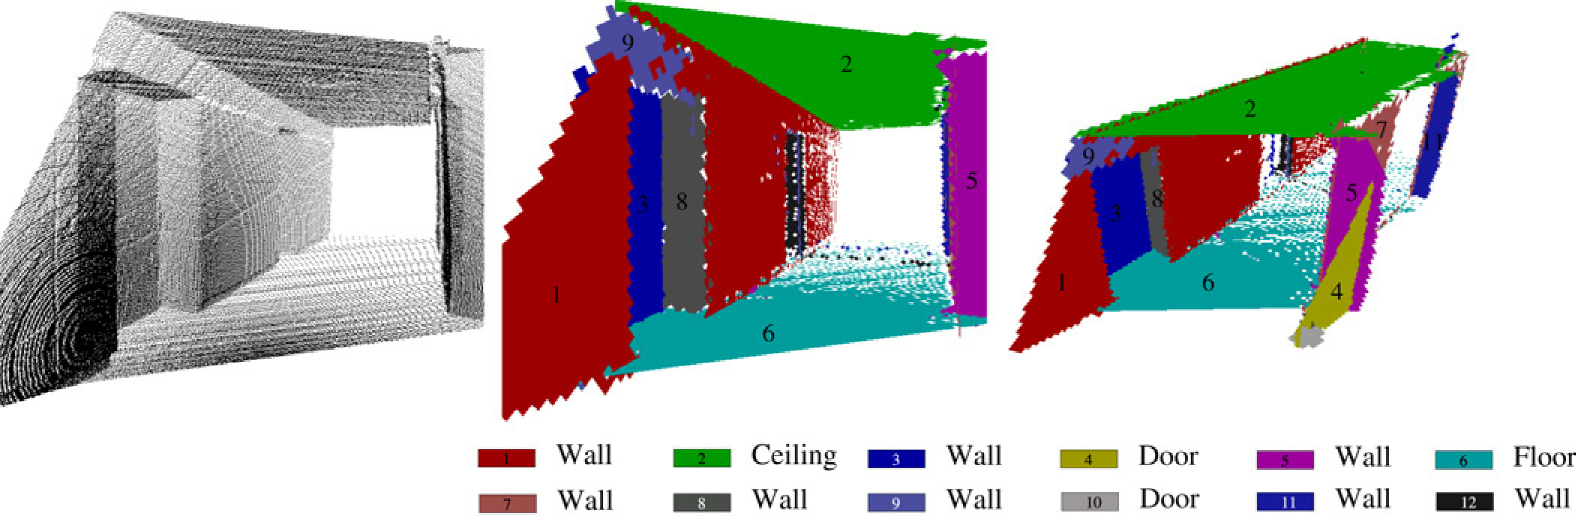
\includegraphics[width=0.9\columnwidth]{typology/semanticmaps_hertzberg.png}
    \caption{Example of a semantic map, taken from~\cite{Nuechter2008}.}
    \label{fig|semanticmap}
\end{figure}

\subsubsection{Intrinsic motivation and curiosity}

The reasons for a robot to acquire knowledge are diverse, and usually external
to the robot itself. It is often driven by the requirements of tasks that the
robot has to execute. In this case, motivations are managed by the execution
controller and are mostly invisible to the knowledge representation system.

However, motivation can also be intrinsic, driven by the internal state of the
robot's beliefs, without external pressure or reward. In this case, the \fxwarning{to be completed}

In the context of robotics, Oudeyer notes however that \emph{the information that is
compared \emph{[to compute a level of motivation]} has to be understood in an
information theoretic perspective, in which what is considered is the intrinsic
mathematical structure of the values of stimuli, independently of their
meaning.}~\cite{Oudeyer2007}.

Psychological grounds of motivation are summarized in~\cite{Oudeyer2007} while
the main approaches to computational motivation, divided into knowledge based
models, competence based models and morphological models, are surveyed
in~\cite{Oudeyer2008}.

%%%%%%%%%%%%%%%%%
\subsection{Practical integration in robotic architectures}
\label{sect|integration-robot}

\begin{scriptsize}
\begin{center}
\begin{tikzpicture}[taxonomy]
    \node [taxon] {\bf E. Integration}
            child {node [taxon] {{\bf E.4} Performances}}
            child {node [taxon] {{\bf E.3} Monitoring}}
            child {node [taxon] {{\bf E.2} Executive layers}}
            child {node [taxon] {{\bf E.1} Sensori-motor}};
\end{tikzpicture}
\end{center}
\end{scriptsize}


Knowledge representation systems do not mean anything to robots if they are
considered in isolation. This section proposes categories of features related
to the integration of the KRS into a larger software architecture that includes
perception routines, decision-making processes and actuation control.

We also mention some practical aspects of a real-world system, like
performances and monitoring tools that come along with the KRS.

\subsubsection{Integration with sensori-motor layers}
\label{sect|integration-sensorimotor}

We have previously discussed (section~\ref{sect|grounding}) the principles of
the grounding process that aims at establishing and maintaining a connection
between percepts (and to a lesser extend, low-level actions) and symbols.

While every real-world cognitive robot need some kind of grounding, the actual
implementations lead to very different information flows.

The systems can be roughly split into two classes: \emph{passive} knowledge
repositories that process symbolic facts produced by lower-level sensori-motor
layers (\emph{push} flow); \emph{active} knowledge managers that directly query
(possibly by polling or on-demand) low-level layers.

This macroscopic distinction is however mostly a matter of defining the
frontiers of the KRS: some systems like KnowRob~\cite{Tenorth2009a} encompass
geometric reasoning layers that would be considered as external by other
systems like ORO~\cite{Lemaignan2010} that focus on the symbolic fact storage
and rely on a ecosystem of independent modules to provide and consume symbolic
knowledge.

\fxwarning{Some archi with the ability to ``listen'' to the robot internal
structures -> which ones?}

Other systems do not fit either in such a partition between active and passive
systems because they do not stand as independent modules but exist as diffuse,
\emph{ubiquitous} knowledge manipulation system (case of the CAST knowledge
model~\cite{Jacobsson2008}), for instance because they are primarily
language~\cite{Ferrein2008, Sabri2011}.

\subsubsection{Integration with executive layers}
\label{sect|integration-executive-layers}

Conversely, the knowledge management module need a tight integration with the
decision-making processes. As for the integration with sensori-motor
layers, the borders of the KRS can be fuzzy and vary from one architecture to
another: many consider symbolic task planning as an integral role of the KRS,
while other have dedicated extensions for planning, some integrate learning as
an on-the-flight process that is part of the KRS, others as an independent
deliberative process, etc.

The actual integration techniques vary also widely, from language extensions
(like the integration of CRAM~\cite{Beetz2010} with KnowRob) and client-server
architectures, to event-driven models (SHARY and ORO~\cite{Alami2011}). Choices
at this level have notable consequences on the whole design of the upper
control architecture of the robot, in particular regarding its modularity and
the ease of addition of new components.

\subsubsection{Monitoring and debugging}
\label{sect|debugging}

It is common to have knowledge representation systems at the heart of a
cognitive robotic architecture, and therefore KRS are easily ``buried'' in the
system.

At the same time, the symbolic model often provides a valuable synthetic view
on the whole state of the robot, furthermore easily understandable by the human
developer (the fact \stmt{human1 isSitting true} is easier to interpret than
the suite of relative coordinates of each joints of the human skeleton, as
provided by the human tracker, for instance).

Tools to trace and visualise at run-time the evolution of the knowledge
structure and contents may be available with the KRS, as well as
post-processing tools that run on the trace to analyze {\it a posteriori} the
cognitive behaviour of the robot.

\subsubsection{Evaluation of performances}
\label{sect|performances}

Benchmarks of symbolic systems for robots are hard to conduct for several
reasons: identifying good metrics for robotic experiments in general is
difficult because of the complex interactions between tenth of modules running
in parallel, and isolating one specific component is difficult.  Also,
knowledge representation systems are often tightly coupled to the other
modules. To quote Langley~\cite{Langley2006}:

\begin{quote}
The conventional wisdom of software engineering is that one should
develop independent modules that have minimal interaction. In contrast, a
cognitive architecture offers a \emph{unified} theory of cognition with tightly
interleaved modules that support synergistic effects.
\end{quote}

The lack of standard API for knowledge services makes it also hard to switch
between KRS to compare them.

Finally, because service robots are designed to act in rich, dynamic
environments, possibly with humans, building repeatable experiments is
challenging, and quantitative measurements are often not the right
metric~\cite{Langley2006}.

We will however present here some quantitative metrics (related to scalability,
for instance), followed by qualitative evaluation approaches, grouped under the
term \emph{Cognitive Performances}.

\begin{scriptsize}
\begin{center}
\begin{tikzpicture}[taxonomy]
    \node [taxon] {\bf E.4 Performance \\Evaluation}
            child {node [taxon] {{\bf E.4.2} Cognitive Performances}}
            child {node [taxon] {{\bf E.4.1} Raw Performances}};
 \end{tikzpicture}
\end{center}
\end{scriptsize}


\paragraph{Raw Performances} The \emph{raw performance} is evaluated on
quantitative benchmarks. The main metric is the \emph{scalability}
$\mathcal{S}^{KRS}$ of the system with the size of the knowledge base
$\sigma=|\Delta^{\mathcal{I}}|$  (in term of atoms or statements).

We call \emph{relaxation time} $\mathcal{R}^{\mathcal{M}}$ the (averaged) time
required by the system after a model modification of type $\mathcal{M}$ before
being available for further interaction, and \emph{query time}
$\mathcal{Q}^{\mathcal{M}'}$ the (averaged) time to execute a query of
complexity $\mathcal{C}$ on the KRS. The type $\mathcal{M}$ of model
alteration is either an ABox modification (addition/removal of an instance) or
a TBox alteration (addition/removal of a class, a class restriction or a rule).
%Query complexity $\mathcal{C}$ is...\fxwarning{find references}.

\emph{Temporal scalability} is defined in term of the nature of the function
$f^{\mathcal{M}, \mathcal{C}}(\sigma) = \mathcal{R}^{\mathcal{M}}(\sigma) +
\mathcal{Q}^{\mathcal{C}}(\sigma)$ (\ie the relation of the relaxation time
and query time to the knowledge base size). \emph{Space scalability} is the
relation of memory consumption to the size $\sigma$. The scalability is tightly
coupled to the expressiveness of the underlying knowledge model, which need to
be known for the scalability measurement to be meaningful.

Because of coupling and repeatability issues we have mentioned, raw
performances of KRS are often benchmarked with synthetic datasets (which leads
to another issues: how to assess the meaningfulness of the performance of a
reasoner on an artificial ontology?~\cite{Bail2010}) or ``toy'' experiments
that do not always model the whole complexity of real-world
application~\cite{Chong2009}.

\paragraph{Cognitive Performances} While evaluating the raw performances of
knowledge representation systems in a relevant manner may be difficult, the cognitive
performances of the robot as a whole can be also evaluated.

Langley et al.~\cite{Langley2006} propose five such dimensions of evaluation:
the \emph{generality} of the system (can it adapt easily to new tasks?), the
\emph{rationality} or relevant of the inference/reasoning/decisions the system
take, the \emph{reactivity} and \emph{persistence} that evaluates if the
behaviour of a cognitive system is appropriate under unpredicted changes, the
\emph{improvability} of the system as a function of the knowledge added to it,
and finally, the resulting \emph{autonomy} of the system.

Cognitive performance can also be evaluated with the support of tools developed
in cognitive psychology. Several standard tests (like False-Belief
experiments~\cite{Leslie2000} or the Token test~\cite{DiSimoni1978}) have been
used to judge the cognitive abilities of robots~\cite{Mavridis2006,
Breazeal2006}.
%%%%%%%%%%%%%%%%%%%%%%%%%%
\subsection{Knowledge instantiation}

\begin{scriptsize}
\begin{center}
\begin{tikzpicture}[taxonomy]
    \node [taxon] {\bf F. Knowledge instantiation}
            child {node [taxon] {{\bf F.4} Granularity}}
            child {node [taxon] {{\bf F.3} Metrics}}
            child {node [taxon] {{\bf F.2} Common-sense and Alignement}}
            child {node [taxon] {{\bf F.1} Design Strategy}};
 \end{tikzpicture}
\end{center}
\end{scriptsize}

This last branch of our taxonomy looks at the actual \emph{content} of the
knowledge base: the knowledge instantiation. Here, \emph{instantiation} does
not only refer to the instantiation of the knowledge structure (what we have
called the ABox), but also includes the knowledge structure itself (the TBox).

While we have previously mentioned features of knowledge representation systems
that enable the robot to fill its knowledge base with content and alter the
knowledge structure, most of the systems also come with a certain amount of
initial knowledge that often includes \emph{common-sense} knowledge (\ie facts
that widely known to humans, and hence often implicit: ``to put a cake in the
oven, one must first open the oven's door'').

The design strategy, the choice to rely on common-sense knowledge or not, the
reuse of standard ontologies, the quantity of {\it a priori} knowledge are many
parameters that lead to different knowledge models.

\subsubsection{Design strategy}
\label{sect|design-strategies}

The main challenge of knowledge representation can be summarised as \emph{How
to model the real-world state and interactions in a symbolic way, processable
by the robot to make decisions}. We have already introduced the term
\emph{grounding} to describe the (bi-directional) process of binding percepts
to symbols.

We have also seen that the instantiation of the knowledge (\ie, the actual,
practical knowledge available to the robot) comes either from some variant of
perception plus grounding, or from knowledge that the developer considers as
already meaningful for the robot: remote semantic databases or initial
(common-sense or situation specific) knowledge.

This translates into two main strategies to drive knowledge instantiation: a
\emph{top-down} design or a \emph{bottom-up} design.

A bottom-up approach to knowledge instantiation takes the output of sensors as
the primary source of knowledge: instances of objects, agents, and their
relations directly result from what is perceived. No abstract, ``from the more
generic to the more specific'' process takes place.

Steels~\cite{Steels2007} considers this approach to be a solved issue, and
according to Sloman~\cite{Sloman2007} (and his stance against the
\emph{``Symbol Grounding meme''}), since bottom-up grounding boils down to grounding
of \emph{somatic} concepts (\ie roughly, the sensori-motor relationships that
the robot learns from its interaction with the world), it constrains in an
unacceptable way the range of concepts accessible to the robot.

Knowledge instantiation can also be approached as a \emph{top-down} activity:
in natural language grounding, for instance, the robot needs to automatically
bind an abstract representation (a group of words uttered by a human) to an
unambiguous, context-dependent, internal concept. This concept may (or may not)
be \textit{a priori} available to the robot as a pre-loaded ontology (what we
previously called the cultural background of the robot). In any case, the robot
must conduct a cognitive process that leads from an abstract concept to a
concrete entity.

The bottom-up and top-down strategies also reflect how the knowledge structure
itself is constructed: either by successive classification and refinement of
percepts, or from generic categories, typically extracted from standard
upper-ontologies.

\subsubsection{Common-sense and alignment with standard upper-ontologies}

At section~\ref{sect|lod} we have presented how remote knowledge bases are a
valuable source of knowledge, including common-sense knowledge, that robot can
extract.

Building {\it a priori} knowledge with a top-down strategy leads to populate
the upper part of the taxonomy with abstract concepts like \emph{Thing},
\emph{Time}, \emph{Person}, etc. The organisation of the whole knowledge
depends on the design of this abstract part of the common-sense knowledge.

Different knowledge structures at this level can lead to serious
misunderstanding: for instance, if one robot considers the concept of a
\emph{person} as representing some intelligent, possibly disembodied, entity,
and another robot represents a \emph{person} as a subclass of mammals, their
models of the world are likely to be conflicting.

To be able to successfully exchange knowledge with other systems (robots,
databases, natural language parsers, etc.), the common-sense knowledge of
robots is thus often aligned with a standard upper-ontology.

Many such upper-ontologies exist (table~\ref{table|upper_onto_metrics} lists
some of them). While {\sc Cyc} and SUMO are current the main two, many efforts
take place to make these ontologies compatible with each other (in particular
by using the {\sc WordNet} thesaurus as intermediate unambiguous source of
semantics).

\subsubsection{Metrics and quality criteria}

Qualitative and quantitative metrics give an insight on the size, complexity
and effectiveness of ontologies used with the robots.

Table~\ref{table|upper_onto_metrics} gives such metrics for five major
upper-ontologies commonly used in the semantic Web community (taken
from~\cite{Mascardi2007} and the projects' respective websites). It is
interesting to note the large variations between projects like {\sc DBpedia}
whose content is automatically generated from Wikipedia, {\sc Cyc} or {\sc
SUMO}, which are both hand written, but do not adopt the same strategy to
select the knowledge to represent.

These metrics do not reflect adequately the \emph{expressive complexity},
though: in most of these ontologies with a large amount of terms and
assertions, taxonomic relations (\concept{isA}) or technical predicates (URI,
translations, etc.) account for a large part of the assertions, at the expense
of real semantic relations.

\begin{table}
\begin{center}

\begin{tabular}{llllll}
\toprule
{\bf Project} & {\bf Terms} & {\bf Assertions} (triples) \\
\midrule
{\sc Cyc} & > 300 000 & > 3 000 000 & \\
YAGO & > 10 000 000 & > 120 000 000 \\
SUMO & 20 000 & 60 000 \\
{\sc DBpedia} (for English) & 1 840 000 & 385 000 000\\
{\sc OpenMind} Common Sense (for English) & & 1 000 000\\
\bottomrule

\end{tabular}
\end{center}
\caption{Raw size of major upper-ontologies.}
\label{table|upper_onto_metrics}
\end{table}

Other metrics that include the type of predicates that are used, or the
computed DL expressiveness, can be more significant (some are presented in
table~\ref{table|onto-stats}, page~\pageref{table|onto-stats}).

Qualitative evaluation of ontologies is also a well studied field. In Staab's
{\it Handbook on Ontologies}, Vrande{\v{c}}i{\'c}~\cite{Vrandevcic2009}
provides a synthesis of qualitative criteria for ontology assessment.  He lists
eight of them: \emph{accuracy, adaptability, clarity, completeness,
computational efficiency, conciseness, consistency,} and
\emph{organizational fitness}. Details and relevant literature can be found
in Vrande{\v{c}}i{\'c}'s chapter.

\subsubsection{Granularity}

Amongst the characteristics of ontologies, knowledge \emph{granularity}
qualifies the level of details or refinement of the knowledge stored. The level
of granularity of a robot's ontology hints on the place of the symbolic layer
in the whole robotic architecture: some systems (like OMRKF~\cite{Suh2007}) go
as down as storing SIFT features (\ie a large volume of numerical values) in
the ontology. The storage of literal values is indeed a relevant case for
robotics. Depending on the representation language, literal values can be
naturally represented and processed (common case in logic programming language)
or not (storing numerical value, let alone matrices, in OWL is cumbersome and
not efficient due to the serialisation to XML).

The issue of the granularity of models can also be partially addressed by
splitting the knowledge representation into a geometric level (where all
numerical values are stored) and a purely symbolic level. The communication
between the two layers is however a complex question.

It must finally be noted that complex robotic systems are likely to use
different level of the knowledge depending on the task to achieve, and the
granularity of the knowledge should probably be considered as a dynamic
property.


%%%%%%%%%%%%%%%%%%%%%%%%%%%%%%%%%%%%%%%%%%%%%%%%%%%%%%%%%%%%%%%%%%%%%%%%%%%%%%%%%%%%%%%%%%%
\section{Existing systems for knowledge representation in service robotics}
\label{sect|surveyed-systems}


Table \ref{table|surveyed-systems} lists the knowledge representation
systems that we have surveyed.

This section first clarify the inclusion criteria, and then briefly presents
each of them. At chapter~\ref{chapt|evaluation}, we will consider again these
systems, this time as a whole, to build a summary of the fields of knowledge
representation that are adequately (or not) tackled by the existing systems.

\begin{landscape}
\begin{table}\scriptsize
\begin{center}

\begin{tabular}{p{2.2cm}p{1.6cm}p{4cm}lp{2.4cm}p{3.4cm}p{1.5cm}}
\toprule
{\bf Project} & {\bf Category} & {\bf Authors (Institution)} & {\bf Project homepage} & {\bf Programming language} & {\bf Knowledge model/Logical Formalism} & Main reference \\
\midrule
ARMAR/Tapas & Formal & Holzapfel, Waibel \par (Karlsruhe TH) & & & TFS (Typed Feature Structures) & \cite{Holzapfel2008}\\
CAST Proxies & Ubiquitous & Wyatt, Hawes, Jacobsson, Kruijff (Brimingham Univ., DFKI Saarbrücken) & & & Amodal proxies & \cite{Jacobsson2008} \\
GSM & Structural & Mavridis, Roy \par (MIT MediaLab) & & & & \cite{Mavridis2006} \\
Ke Jia Project & Formal & Chen et al. \par (Univ. of Science and Technology of China) & \url{www.wrighteagle.org/en} & ASP (Answer Set Programming) & ASP & \cite{Chen2010} \\
{\sc KnowRob} & Formal & Tenorth, Beetz \par (TU Munich) & \url{ias.in.tum.de/kb/wiki} & {\sc Prolog} & {\sc Prolog} + OWL-DL &  \cite{Tenorth2009a} \\
NKRL & Language & Zarri et al. \par (Paris Est Créteil Univ.) & & NKRL & & \cite{Sabri2011} \\
%OBOC & KRS & Mendoza & & & & & \cite{Mendoza2005} \\
OUR-K/OMRKF & Formal & Lim, Suh et al. \par (Hanyang Univ.) & \url{incorl.hanyang.ac.kr/xe} & ? & DL + Horn Clauses &  \cite{Lim2011, Suh2007} \\
%ORO & KRS & Lemaignan, Alami \par (LAAS-CNRS) & \url{oro.openrobots.org} & {\sc Java} & OWL-DL ({\sc Jena}) & {\sc Pellet} & \cite{Lemaignan2010} \\
PEIS KR\&R & Formal & Daoutis, Coradeshi, Loutfi, Saffiotti \par (Örebro Univ.) & \url{www.aass.oru.se/~peis} & {\sc C}, {\sc CycL} & CycL (1st and 2nd order logics, modal logics) & \cite{Daoutis2009} \\
%Golog & Language & Levesque (Toronto Univ.) & & {\sc Prolog} & & & \\
% & & Varadarajan, Vincze \par (TU Wien) & & & & & \cite{Varadarajan2011} \\ % -> affordances, but no implementation on a robot
% & & Kaelbling, Lozano-Pérez \par (MIT CSAIL) & & & & & \cite{Kaelbling2011} \\ % -> mostly planning under uncertainty
% & & Hertzberg (Osnabrück Univ.) \\ % -> affordances, semantic mapping
% (based on {\sc KnowRob} & & (JSK) \\

\bottomrule

\end{tabular}
\end{center}

\caption{List of surveyed systems. Categories are \emph{Formal} for systems
that have a formal underlying knowledge representation, \emph{Ubiquitous} for
systems where knowledge is fully distributed, \emph{Language} for languages
used as KRS on robots or \emph{Structural} for KRS where knowledge is
represented as special data structures.}

\label{table|surveyed-systems}
\end{table}
\end{landscape}

\subsection*{Survey Inclusion Criteria}
\label{sect|inclusion-criteria}

Every robotic system has, implicitly or not, some knowledge representation
systems. It may range from a simple state vector to an explicit symbolic
knowledge base.  This survey focuses on the right end of this spectrum:
symbolic systems, suited for abstract reasoning.

Besides, we have decided to restraint the set of systems to those actually
implemented on robots, and used in semantic-rich environments (\ie dynamic,
partially unknown environments with a large range of different entities which
may have interactions). The typical scenario that would involve such robots
is the \emph{Brownie Scenario} already presented at
section~\ref{sect|scenario}: a service robot in a human-friendly environment
like a kitchen.

We have limited ourselves to systems that
\begin{inparaenum} 
    \item  run on \emph{service robot} (that is, robots that interact with 
    objects in a semantic-rich environment primarily designed for humans),
    \item  ground the knowledge in the physical world (physically embedded
    systems able to assess their environment),
    \item  are able to merge different knowledge modalities,
    \item  are able of on-line, dynamic knowledge acquisition and reasoning 
    (\ie not simple static databases).
\end{inparaenum}

These criteria exclude platforms like {\sc DyKnow}~\cite{Heintz2004}
which are focused on data fusion and knowledge grounding at lower levels.

We have also chosen not to include the GOLOG language and its
derivatives~\cite{Levesque1997, Ferrein2008, Gspandl2011} in this survey. While
several implementations on robots, including service robots, do exist, the
focus of this language is on representation and reasoning about actions and
situations, and the link with symbolic, abstract knowledge is not explicit.

While classical cognitive architectures like {\sc Soar}~\cite{Lehman2006},
GLAIR~\cite{Shapiro2009} or {\sc ACT-R} have declarative knowledge
modules~\cite{Derbinsky2010} and have been recently used on service robots (see
{\sc ACT-R/E}~\cite{Kennedy2009} for instance), they are also absent from this
survey because we did not find much references in the literature on knowledge
manipulation and representation applied to real-world robotic scenarii for
these architectures.

A comprehensive reference on (bio-inspired) cognitive architectures is also
available from the BICA Society~\cite{BicaCogArch2011}.

\subsection{ARMAR/Tapas}

{\sc Tapas} is the name of the knowledge representation system and dialogue
manager found on the ARMAR~III robot~\cite{Holzapfel2008} for the Karlsruhe
Institute of Technology.

Knowledge in {\sc Tapas} exists as procedural knowledge (plans) and declarative
knowledge. The later is split into \emph{lexical knowledge}, \emph{semantic
knowledge} and a database of identified objects (with their properties). The
\emph{lexical knowledge} contains lexical and grammatical informations about
the objects. The \emph{semantic knowledge} is organised into an ontology
relying on \emph{typed feature structures} (TFS~\cite{Carpenter1992}, a
formalism originating from the computational linguistics community, and a
superset of first-order logic).

{\sc Tapas} has a strong focus on natural language grounding. It proceeds by
generating grammars from properties represented in the ontology to parse and
understand dialogue.

Another focus is put on handling unknown words and objects. {\sc Tapas}
provides routines to recognise unknown entities, and propose and interactive
and iterative verbal process to categorise (including adding new categories)
those new concepts.

\paragraph{Experiments} {\sc Tapas} has been used experimentally in a kitchen
environment where naive users had to ask the robot for an object and get
information about another object.

\subsection{CAST knowledge model}
\label{sect|cast}

CAS (\emph{CoSy Architecture Schema}) Toolkit~\cite{Hawes2007} is a
comprehensive toolkit aimed at building cognitive architectures for robots
through a set of interconnected \emph{SA} (\emph{subarchitectures}). The CAS
does not expose a central knowledge base as seen in other works. It represents
instead knowledge as unrooted \emph{proxies}. Those proxies are formally
defined in \cite{Jacobsson2008} as $p= \langle F_p, u_p \rangle$ where $F_p$ is
a set of instantiated features (like $\phi^{Colour}_{red}$) and $u_p$ a
\emph{proxies union} that form an equivalence class corresponding to one
entity.

A union of proxies forms a global amodal representation of an entity, that can
be explicitly shared and manipulated. Being not centralised, the knowledge
model can be qualified of \emph{ubiquitous}. Furthermore, knowledge source in
the CAS architecture is tightly bound to the on-line grounding process (be it
grounded in perception or in dialogue). While nothing seems to prevent it, no
{\it a priori} knowledge (including common-sense knowledge) is used.

Knowledge sharing is ensured by the event mechanism of CAST: modules can
monitor proxies for alteration by other modules. Jacobsson et al. mention how
this can apply to reinforcement learning: the vision module creates a proxy for
an orange object. This proxy get monitored by a learning module. In parallel,
the proxy is bound to an union by the natural language understanding module
that add new a feature like \emph{"this object is a fruit"}. The learning
module is called back, and can add this new information to its model.

In the presented implementation, the CAST knowledge model does no allow for
effectively representing actions or temporal information.\fxwarning{What about
reasoning? can they retrieve for example 'all proxies for colorful objects'?}

\paragraph{Knowledge Acquisition} Several techniques for knowledge acquisition
have been explored within the CAST framework. Cross-modal knowledge
fusion~\cite{Hawes2007a} is well studied, and the interaction with natural
language processing~\cite{Kruijff2010, Kruijff2010a} is a particular emphasise
of the project.

In~\cite{Hawes2011}, Hawes et al. also explore \emph{curiosity} mechanisms in
the context of spatial representations with the robot \emph{Dora}.

\paragraph{Experiments} CAST has been used in several experiments, including
table-top manipulation (with a focus on language understanding) and more
recently on the Dora robot~\cite{Hawes2011} for indoor exploration.

\subsection{GSM}
\label{sect|gsm}

GSM (for \emph{Grounded Situation Model})~\cite{Mavridis2006} is a knowledge
representation system primarily built to ``facilitate cross-modal
interoperability'',  especially in the context of verbal interaction with a
robot.

GSM does not rely on any formal language but rather on a layered data structure
(figure~\ref{fig|gsm}) that organises the surrounding world into agents and
relations between agents.  Each agent (any animate or inanimate object) is
attached to a physical model (made of \emph{body parts} that have properties
like their position, color, etc.) and a mental model (which is a recursively
embedded GSM, thus allowing a sort of theory of mind).

\begin{figure}
    \centering
    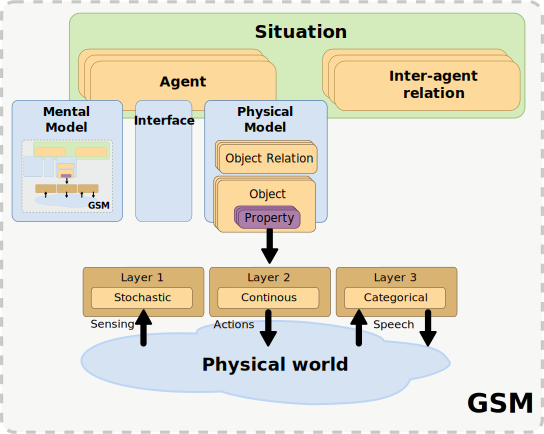
\includegraphics[width=0.65\columnwidth]{stateofart/gsm.pdf}

    \caption{Simplified hierarchical structure of the Grounded Situation Model,
    based on~\cite{Mavridis2006}.}

    \label{fig|gsm}
\end{figure}

Properties are represented in three layers: a stochastic representation, close
to sensory percepts, a \emph{continuous single-valued} encoding of the
stochastic model, and a discrete, categorical model.

One notable feature of GSM is the \emph{bidirectionality} of the grounding
process: not only sensor percepts are abstracted into categories suitable for
human conversation, but human utterance (like ``There is a red ball in the
center of the table'') can also be turned into property descriptions. This
basically enable the knowledge representation system of the robot to
\emph{imagine} entities.

GSM also features several strategies for managing time and events.
\emph{Moments} are created by storing timestamped snap-shots of GSM, and
\emph{event classifiers} allow to define and detect events.

\paragraph{Experiments} GSM has mostly been tested on table-top manipulation
and interaction tasks (a ``conversational helping hand'' as stated by the
authors) implemented on a 7-DOF arm equipped with force feedback, cameras for blob
tracking and speech recognition (Sphinx4). Mavridis and Roy provide in addition
an in-depth analysis of the performance of GSM by the mean of a standard
psycholinguistic test, the \emph{Token test}~\cite{DiSimoni1978}.

\subsection{Ke Jia Project}
\label{sect|kejia}

The Ke Jia project~\cite{Chen2010} integrates on a mobile platform a knowledge
representation language with natural language processing, task planing and
motion planing.

Knowledge representation relies on \emph{Action Language C}, itself based on
\emph{Answer Set Programming} (ASP)~\cite{Gelfond2008}. These languages, that
are syntactically close to Prolog, are based on \emph{stable models} of logic
programs, and support non-monotonic reasoning. Default and non-monotonic
reasoning has been especially researched within the Ke Jia project for symbolic
task planing~\cite{Ji2011} and underspecified natural language processing.

Amongst other features, the natural language processing capabilities of the
system support acquisition of new logical rules at run-time.

\paragraph{Experiments} The Ke Jia robot has been demonstrated in several tasks
involving human-robot interaction with natural language. These tasks include a
task with multiple \emph{pick \& carry} that are globally optimised, naive
physics reasoning via taught rules or more complex scenarii with the robot
delivering drinks, taking into account changing and mutually exclusive
preferences of users.


\subsection{KnowRob}
\label{sect|knowrob}


{\sc KnowRob}~\cite{Tenorth2009a} is an integrated knowledge management system
developed at the Technical University of Munich. It is build as a set of
modules (figure~\ref{fig|knowrob} organised around a core reasoning system
written in Prolog. This core module interfaces through Java/Prolog or
C/Prolog APIs with external modules.

\begin{figure}
    \centering
    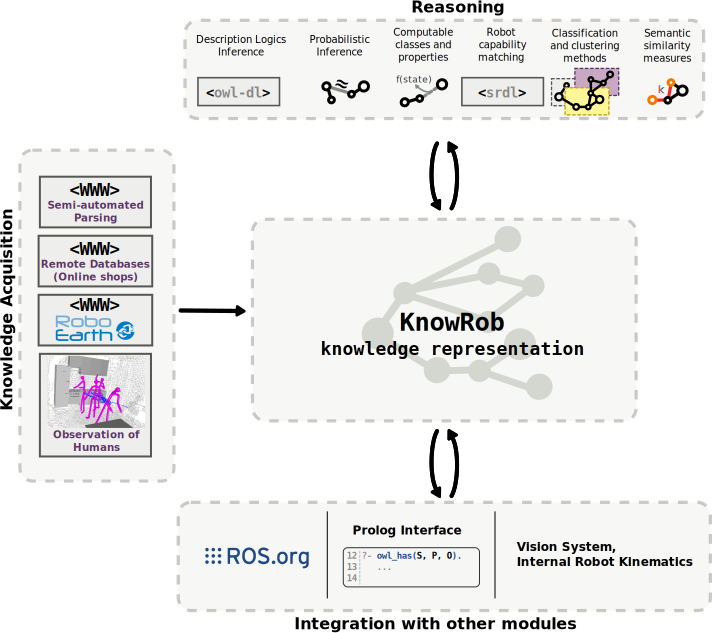
\includegraphics[width=0.7\columnwidth]{stateofart/knowrob.pdf}

    \caption{Overview of the {\sc KnowRob} framework, taken
    from~\cite{Tenorth2011}.}

    \label{fig|knowrob}
\end{figure}

Extension modules can plug into the system to provide specialised reasoning
capabilities or interfaces to external data sources, \eg to read object
detections from the vision system. These modules operate on the level of
instances (ABox).

\paragraph{Knowledge model} {\sc KnowRob} can load OWL ontologies, and the
\emph{KnowRob-Base} ontology is provided as a common-sense ontology, with a
focus on household and kitchen domains. {\sc KnowRob} also store and reason on
introspective knowledge through the \emph{Semantic Robot Description
Language}~\cite{Kunze2011} that allow to represent symbolically the
capabilities of the robot, and is used for planning.


\paragraph{Reasoning Techniques} Amongst the notable {\sc KnowRob} extensions,
{\sc ProbCog}~\cite{Jain2009} is an effort to provide probabilistic reasoning
based on bayesian networks, integration with naive physics reasoning has been
studied~\cite{Kunze2011a}, automatic parsing of Web resources in semi-natural
language has been also experimented with~\cite{Nyga2009}.

\paragraph{Grounding} {\sc KnowRob} offers a mechanism called \emph{computables} that allow to
evaluate certain predicates by calling external dedicated functions (for
instance, the valuation of a proposition like \stmt{object1 isOn object2} is
computed when required by calling a specific geometric reasoning module). In
combination with Prolog's lazy evaluation strategy, this supports a good
scalability.

Computables rely on various subsystem to evaluate. In particular, it relies on
the CoP framework~\cite{Klank2009} and \emph{semantic maps}~\cite{Blodow2011}
for the recognition of objects and environment.

%\paragraph{Integration with Decisional Layers} CRAM~\cite{Beetz2010}

\paragraph{Experiments} {\sc KnowRob} has been deployed on several scenarii at
the Technical University of Munich, on the PR2 robot and on a 2-arm custom
mobile manipulator in the scope of the ``assistive kitchen''~\cite{Beetz2008}
project. These experiments include retrieval and automated parsing of recipies
from the Web, retrieval and manipulation of various kitchen tools, cooperation
between two robots.

\subsection{NKRL}
\label{sect|nkrl}

\emph{NKRL} stands for \emph{Narrative Knowledge Representation Language}.
While this language is developed since a long time by Zarri~\cite{Zarri1997,
Zarri2008}, recent research direction include application to the robotic
field~\cite{Sabri2011}. NKRL is not {\it per-se} a knowledge representation
system, as it is primarily a language. However, it is used as the
representation and reasoning mechanism for robots by Sabri et al.

\paragraph{Knowledge representation} The NKRL language semantics are stored in
two ontologies: an ontology of concepts $\Omega$ and an ontology of events
$\Psi$. The ontology of events is made of action or situation templates.
Templates are a set of predicates (MOVE, PRODUCE, RECEIVE, EXPERIENCE, BEHAVE,
OWN and EXIST) associated to thematic roles. Grounding and reasoning with NKRL
is based on template matching.

\paragraph{Experiments} The main scenario of development for NKRL-based robots
is the Smart Home and monitoring of eldery people. Knowledge acquisition
partially rely on ambient intelligence (RFID, pressure sensors in the chairs,
etc.). The scenario is still being implementated.

\subsection{OUR-K and OMRKF}
\label{sect|omrkf}

The Ontology-based Unified Robot Knowledge~\cite{Lim2011} (OUR-K) framework,
successor of the Ontology-based Multi-layered Robot Knowledge
Framework~\cite{Suh2007} (OMRKF), is a knowledge representation system based on
five inter-related \emph{classes} of knowledge (figure~\ref{fig|omrkf}). It
proposes a layered approach to knowledge representation that allows to
integrate the grounding process to the knowledge representation process. OUR-K
knowledge model is implemented with a mix of Description Logics for the concept
hierarchies and Horn clauses.

\begin{figure}
    \centering
    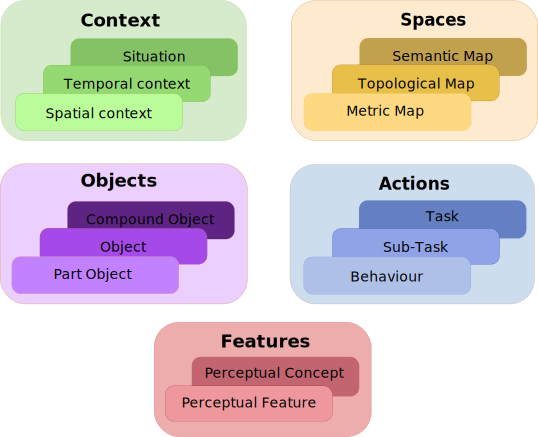
\includegraphics[width=0.5\columnwidth]{stateofart/ourk.pdf}

    \caption{OUR-K organises knowledge into fives \emph{classes}, each composed
    of \emph{levels}. Figure based on~\cite{Lim2011}.}

    \label{fig|omrkf}
\end{figure}

Each level of knowledge is build as three stages of ontological realization: a
\emph{meta-concept} (the level itself, like ``temporal context'', ``behaviour''
or ``object feature''), a taxonomy of concepts inside this level (for instance
$cup : Object \sqsubseteq tableware : Object$) and an instantiation of the
taxonomy ($cup1 : cup$).

\paragraph{Representation} The environment is represented in OUR-K in the
$spaces : Model$ knowledge level as a classical three layers mapping (metric,
topological and semantic maps). Objects (in $objects : Model$) are localised in
$spaces : Model$ through Voronoi nodes.

The knowledge class $Context$ proposes an explicit statement of spatial context
(mostly geometric relations between objects), temporal context and a more
general \emph{high-level} context, inferred from spatial and temporal contexts.

Finally, the $Activity$ knowledge class store compound actions in a HTN-like
structure, exploited at run-time by a planner.

\fxwarning{re-read the paper to improve the section...}

\paragraph{Experiments} Experiments conducted with OUR-K and OMRKF include
finding kitchen objects and reporting about their state to a human.  This
experiment also shows how OUR-K can deal with objects only partially matched by
their descriptor by introducing a $candidate()$ function.

\subsection{PEIS KR\&R}
\label{sect|peis-ecology}

{\sc PEIS Ecology}~\cite{Saffiotti2005} is a software \emph{ecosystem} that aim
to binds autonomous robotics with ambient intelligence (network of sensors).
\emph{PEIS} stands for \emph{Physically Embedded Intelligent System}: every
robots or intelligent device in the environment is abstracted as a PEIS.

Each PEIS physical component is running a \emph{PEIS Kernel} instance.
Communication between instance relies on a custom P2P communication protocol.

The PEIS architecture allows for adding new abilities through software
components sharing the common \emph{tuple space}.

We consider here the semantic layer~\cite{Daoutis2009}, referred as \emph{PEIS
KR\&R}, that includes symbolic representation and reasoning.

\fxwarning{have a look to latest Daoutis paper!}

% More in details:
% - object identification based on viewpoint independent SIFT features
% - formalised anchoring system that explicitly match percieved attributes to predicates
% - Cyc predicates
% - ground 12 colors, based on a paper on color perception. Could be useful for us.
% - idem, they cite a paper on what spatial relations to compute
% - location of objects based on a previously provided semantic map (but not much on this semantic map)
% - two "memories": the robot memory stores the current list of percieved objects ; the archive memory stores what is not percieved anymore
% - uses directly Cyc (ie, 250 000 common sense concepts\ldots), via CycL language -> 2nd and higher order logics (quantification over predicates, functions, etc)
% Remark: using 2nd order logic (ie meta statements), it would be easy to store the knowledge of each agent
% - disambiguation in concept name by asking human to decide amongst all concepts known by Cyc
% - template based natural language
% - experiment conducted in a "smart" indoor environmement + simple robot

\paragraph{Knowledge model} The PEIS Knowledge representation system relies on
the {\sc ResearchCyc} and {\sc CycL} language to represent knowledge. The {\sc CycL} language
allows to represent first order logic sentences and has extensions for modal logics and higher order logics.

\fxwarning{Is modal logics and higher order logics actually used in PEIS?} 

As a system relying on {\sc CycL}, contexts can be expressed as
\emph{microtheories}: the truth or falsity of a set of statement depends of the
\emph{microtheory} in which these statements are evaluated.

\fxwarning{OWA/CWA?}

\begin{figure}
	\centering
	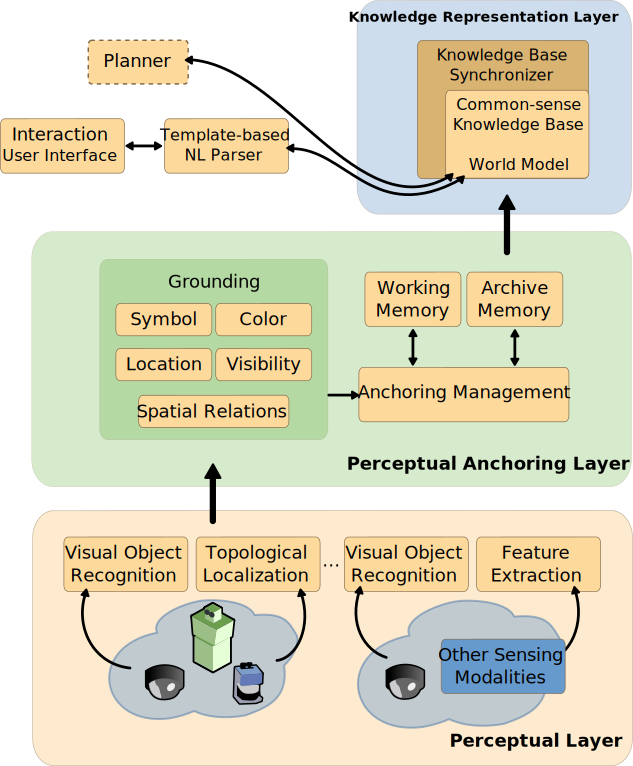
\includegraphics[width=0.5\columnwidth]{stateofart/peis-architecture.pdf}
	\caption{The PEIS knowledge representation system, taken from~\cite{Daoutis2009}}
	\label{fig|peis-archi}
\end{figure}

The PEIS KR\&R system is deeply integrated to the general PEIS Ecology
\emph{smart} environment. Figure~\ref{fig|peis-archi} gives an overview of the
interactions between PEIS knowledge processing layers.

\paragraph{Knowledge Acquisition} The primary source for knowledge acquisition
is perception.  The PEIS ecosystem provides a SIFT-based object recogniser used
in conjunction with ceiling cameras for object localisation.  Other perceptual
modalities are available (like human tracking, ambient environment monitoring).

A template-based natural language parsing system may also be used to add new
assertions to the system.

The system can ask the human for help to disambiguate between concept names.

\paragraph{Anchoring} Daoutis et al. formalise the issue of anchoring as
finding a \emph{predicate grounding relation} $g \subseteq \mathcal{P} \times
\Phi \times D(\Phi)$, where $\mathcal{P}$ is a set of predicate symbols, $\Phi$
a set of percept's attributes, and $D(\Phi)$ the domain of these attributes.

In the current implementation, object category (returned by the SIFT
classifier), color, location, spatial relations (both topological -- \emph{at},
\emph{near} -- and relative to the robot -- \emph{left}, \emph{behind}, etc.)
and visibility are the five classes of extracted attributes.

\paragraph{Integration in the robot architecture}
\label{sect|peis-integration}

The PEIS framework offers through the \emph{PEIS middleware} a practical way to
insert a new component into the shared \emph{tuple space}.  Thus, the KR\&R
module can be seamlessly integrated into the PEIS ecosystem.

\paragraph{Experiments} Experiments involving PEIS take place in a Smart Home
environment (\emph{PEIS Home}). The implemented case studies explore
dialogue-based interaction with the robot about known objects.

%%%%%%%%%%%%%%%%%%%%%%%%%%%%%%%%%%%%%%%%%%%%%%%%%%%%%%%%%%%%%%%%%%%%%%%%%%%%%%%

\section{An interface for knowledge manipulation in robotics}
\label{sect|knowledge-api}

During the preparation of the thesis, discussions with several people involved
in knowledge representation (namely Dominik Jain, Lars Kunze, Michael Beetz)
have led to the draft of a generic API for knowledge access and exchange
between robotics components.

This section presents this effort of standardisation that is (partially)
implemented by the ORO server, presented in the next chapter.

\subsection{Rationale and general considerations}

The original idea comes from the acknowledgement that more and more software
components for robotics want to store or use symbolic data. Since established
international efforts at defining standard for inter-component communication
like ROS have already proved their usefulness, one single API for different
knowledge representation and management systems could be equally useful.

% Two main previous attempts must be mentioned: the \emph{Knowledge Interchange
% Format} (KIF) and the DIG interface.
% 
% \fxfatal{Complete this part}
% The \href{http://dig.sourceforge.net/}{ DIG interface}
% 
% The \href{http://logic.stanford.edu/kif/dpans.html}{ Knowledge Interface Format
% (KIF)}. In~\cite{Ginsberg1991}, Ginsberg explains why \emph{knowledge
% interchange formats} are hardly a good idea.

The API is designed for robotics (even if probably useful in other contexts):
it aims to be simple and practical for clients by focusing on core knowledge
operations (addition of knowledge, retraction, querying) with consistency
constraints; it explicitly supports uncertain knowledge and multiple models
(modality); it makes clear how knowledge is added or retracted with explicit
policies.

We have attempted to design it in a way that do not restrict expressiveness
(any logical sentence that can be expressed in the logic of predicates, with a
probabilistic extension, can be manipulated by the API), and a simple extension
mechanism should permit future evolutions in a backward compatible way.

Besides facilitating exchange of knowledge contents between systems by ensuring
one standard formalism, another outcome of the adoption by several KRS of this
API is that it allows easy switch between semantic engines (and thus
benchmarking and sharing of unit-tests).

This API was developed with Prolog-based knowledge systems, Description
Logics-based knowledge bases and Markov networks in mind, and should cover as
well other systems related to predicate logics (with or without a probabilistic
extension).

Besides standard operations on axioms and taxonomy, the API aims to cover:

\begin{itemize}
    \item  probabilities associated to statements
    \item  management of several models
    \item  explicit policies to add, retract or, more generally, alter 
    knowledge (for instance, to guarantee consistency when adding knowledge)
    \item  specific, implementation-dependent, extensions through the
    \texttt{special} method.
\end{itemize}

Implementations are not always expected to cover to whole API, but must have a
predicable behaviour when a part of the API is not implemented. In particular,
the API makes no assumptions on implementations regarding:

\begin{itemize}
    \item  the actual supported expressiveness (the API allows to express
    general first-order logics statements, but the underlying implementation
    may support only a subset, for instance, Description Logics)
    \item  Closed-world assumption vs Open-world assumption
    \item  Reasoning capabilities
\end{itemize}

\subsection{The Knowledge API}

The API is divided in five parts:
\begin{enumerate}
    \item Methods related to service management,
    \item Methods related to knowledge alteration,
    \item Methods related to knowledge querying,
    \item Methods related to models manipulation and finally
    \item Methods related to taxonomy walking.
\end{enumerate}

Parts 2 and 3 are the two main parts, involved with knowledge manipulation.

\paragraph{Knowledge Alteration} Methods in part 2 are build around the generic
\jmeth{revision} method, that takes as parameter a set of logical propositions
and a policy.

A policy is represented as a set of \texttt{(key, value)} pairs whose possible
values are presented in table~\ref{table|knowledge-policies}.

\begin{table}
\begin{center}

    \begin{tabular}{lp{4cm}p{9cm}}
    \toprule
    Key & Values & Meaning \\
    
    \midrule

    { \tt method} & {\tt add} \emph{(default)} & the statements are added to the
    knowledge base, without ensuring consistency.\\ 
    
    \midrule

    & {\tt safe\_add} & the statements are added only if they (individually) do
    not lead to inconsistencies.\\ 

    \midrule
    
    & {\tt retract} & the statements are removed from the model. Associated
    probabilities are discarded.\\ 
    
    \midrule
    
    &{\tt update} & Updates objects of one or several statements in the
    specified model. If the predicate is not inferred to be \emph{functional}
    (\ie, it accept only one single value), behaves like {\tt add}.\\ 
    
    \midrule
    
    & {\tt revision} or {\tt safe\_update} & Updates objects of one or several
    statements in the specified model if it does not (individually) lead to
    inconsistencies. If the predicate is not inferred to be \emph{functional}
    (\ie, it accepts only one single value), behaves like {\tt safe\_add}.\\ 
    
    \midrule
    
    {\tt model} & {\tt all} \emph{(default)} & all existing \emph{models}
    (section~\ref{sect|kbapi-models}) are impacted by the change.\\

    \midrule
    
    & a valid model id or a set of valid model id & only the specified model(s)
    are impacted\\
    
    \bottomrule
    
    \end{tabular}

\end{center}
\caption{Knowledge revision policies.}
\label{table|knowledge-policies}
\end{table}

\paragraph{Knowledge Querying} The main method that allow for knowledge
retrieval is \jmeth{find}. A \jmeth{find} query is build as a set of partial
statements (\ie, statements with named or anonymous unbound terms) that form a
pattern. It returns statements matching the pattern.

``Shortcut'' methods are offered by the API for common operations
(adding/retracting a statement, checking if a statement exists, etc.). Where
relevant, probabilistic versions of the methods are also defined.

The complete API reference is provided in Appendix~\ref{chapter|kb-api}.

%%%%%%%%%%%%%%%%%%%%%%%%%%%%%%%%%%%%%%%%%%%%%%%%%%%%%%%%%%%%%%%%%%%%%%%
%%%%%%%%%%%%%%%%%%%%%%%%%%%%%%%%%%%%%%%%%%%%%%%%%%%%%%%%%%%%%%%%%%%%%%%

\recap

That concludes the chapter on Symbolic Knowledge Representation for robotics.

In that chapter, we have first discussed a definition of \emph{knowledge} in
our context of service robotics and human-robot interaction. We have presented
several references from the literature regarding the identification and
classification of prominent features of knowledge representation systems. 

We have then introduce a comprehensive typology of such features, that
comprises of about fifty concepts sorted into six main categories: features
related to knowledge expressiveness, features related to representation
techniques, features related to reasoning, features related to acquisition and
grounding of knowledge, features related to the integration of a KRS into a
larger robotic architecture, and finally, features that characterise the
represented knowledge itself. Each of the fifty concepts has been briefly
presented with references to the literature.

Finally, we have surveyed eight systems for knowledge representation in service
robots and underlined their main strengths.

The next chapter introduces ORO, a tenth KRS that we have designed and
implemented during the thesis preparation.


\chapter{The OpenRobots Ontology framework}
\label{chapt|oroserver}

This chapter introduces the \emph{OpenRobots Ontology} server and its
common-sense knowledge base.

We present a \textbf{functional description} of oro-server, and detail at
length its knowledge model. Its actual implementation is discussed in the next
chapter.

We also present in depth the \emph{OpenRobots Common-Sense Ontology} that
contains most of the knowledge at hand when the robot starts.

\section{Functional overview}
\label{sect|functional-overview}


We have adopted a centralised approach for knowledge management called
ORO~\cite{Lemaignan2010}. The platform is designed as a central
knowledge storage service implemented as a server where the robot
components can add or query statements at run-time. Figure~\ref{fig|oro-overview}
illustrates the main functional components of ORO.

\begin{figure}
\centering
  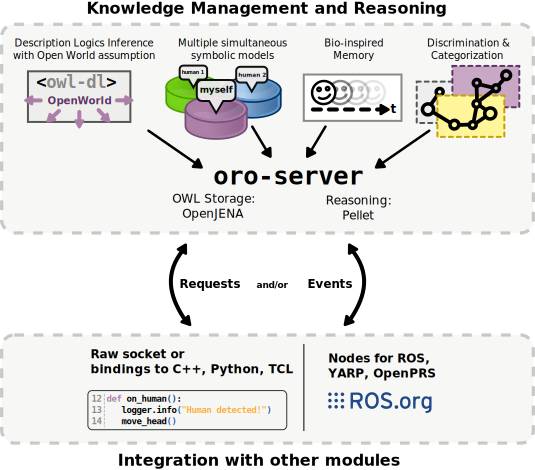
\includegraphics[width=\columnwidth]{oroserver/oro_architecture_functional.pdf}
  \caption{Overview of the ORO architecture.}
  \label{fig|oro-overview}
\end{figure}

At the core, ORO is build around the
OpenJena\footnote{\url{http://www.openjena.org}} ontology management library,
connected to the Pellet\footnote{\url{http://clarkparsia.com/pellet}}
reasoner.

A front-end accepts and manages connections to clients. The clients' requests
are processed by a set of internal modules: basic operations on statements,
but also higher cognitive and human-robot interaction related features
are available. External plugins can also be easily added.

Besides acting as a facts database, the ORO platform exposes several
functions: operations on knowledge statements relying on inference (through a
continuous first-order logic classification process), management of
\emph{per-agent} symbolic models, and also higher cognitive and human-robot
interaction related features like categorisation of sets of concepts
or profiles of memory (that enable the robot to ``forget'' about some facts).

ORO also provides an event mechanism that allows components to be triggered
when specific events occur. A component can for instance subscribe to events
of kind \setstmt{?agent isVisible true, ?agent type Human}. As soon as the
perception layer detects a human in the robot's field of view and accordingly
updates the knowledge base, the executive layer is triggered. The event
framework also takes advantage of the inference capabilities of ORO. Thus an
event can be indirectly triggered if its triggering conditions can be
inferred to be true.



%%%%%%%%%%%%%%%%%%%%%%%%%%%%%%%%%%%%%%%%%%%%%%%%%%%%%%%%%%%%%%%%%%%%%%%%%%%%%%%
%%%%%%%%%%%%%%%%%%%%%%%%%%%%%%%%%%%%%%%%%%%%%%%%%%%%%%%%%%%%%%%%%%%%%%%%%%%%%%%

\section{The ORO Knowledge model}
\label{sect|knowledge-model}

\subsection{Expressiveness}

Unlike systems relying on logic programming like {\sc KnowRob}, ORO is purely
based on Description Logics: the ORO knowledge model is based on RDF triples
(\ie exclusively binary predicates). Triples \stmt{subject predicate object}
are the atoms of knowledge for ORO.

The formal expressiveness of the current version of the ORO common-sense
ontology (commit {\tt 19f1fcf27} in the public repository\footnote{Clonable
from \url{http://git.openrobots.org/git/robots/oro.git}}) is
$\mathcal{SROIQ(D)}$, which correspond to the OWL2 language expressiveness (the
appendix~\ref{chapt|dl} presents the usual naming conventions of Description
Logics expressiveness).

The relation between expressiveness and reasoning complexity is highly
``unstable'': for instance, adding  the single ORO axiom \stmt{farFrom
disjointProperty near} that states that two individuals can not be at the same
time near and far from each other changes the expressiveness power from
$\mathcal{SHOIQ(D)}$ to $\mathcal{SROIQ(D)}$: this seemingly  innocuous
assertion change the complexity class of the whole ontology, and the concept
satisfiability reasoning problem switches from a {\it NExpTime-complete}
problem to a {\it NExpTime-hard} problem (\ie, \emph{at least} as hard as the
hardest problem in {\it NExpTime}).

This instability leads to hard-to-predict run-time performances on the robot,
and light alteration of the knowledge structure can lead to very noticeable
performance drops.

Table~\ref{table|onto-stats}, page~\pageref{table|onto-stats} gives
quantitative details on the type of axioms used in the ORO common-sense
ontology.

\paragraph{Reification} Since RDF triples constraint to binary predicates,
\emph{reification} is often required to express $n$-ary relations. For
instance, the relation \emph{A gives object B to C} can not directly be
represented in RDF. This relation is reified as \{\stmt{act1 type Action},
\stmt{act1 performedBy A}, \stmt{act1 actsOn B}, \stmt{act1 receivedBy C}\}. As
long as the instance \concept{act1} exists in the knowledge base, the original
relation \emph{A gives object B to C} is considered to hold. This kind of
reification is common in the ORO knowledge model.

Reification can also take place at a meta-level (this is the level usually
intended when knowledge manipulation API mention reification): a triple
\stmt{subject predicate object} can be itself reified in \{\stmt{stmt1 type
Statement}, \stmt{stmt1 hasSubject subject}, \stmt{stmt1 hasPredicate
predicate}, \stmt{stmt1 hasObject object}\}. This level of reification allows
to characterise to knowledge atoms themselves, for instance to specify when the
atom was added. The section on memory management in ORO server, below, gives
examples of usage of this meta-cognition feature.

Note that in traditional logical programming like Prolog, reification is rarely
strictly required since no constraints hold on the arity of predicates. To
store the date of creation of a facts, one could simply add it as a
supplementary argument of the predicate\footnote{In the case of time
representation, however, reification --- or, in the case of logic programming,
second order logic --- is commonly found through the \emph{fluents} mechanisms,
see section~\ref{sect|time-representation}}.

\paragraph{Open World Assumption}

%%%%%%%%%%
\subsection{How things are represented?}

\subsubsection{Role Representations}
Spatio-Temporal Representations:

\paragraph{Representation of space}
\paragraph{Representation of events and actions}


\subsubsection{Representation of Alternative Knowledge Models}
\label{sect|alterite}

As pictured in Figure~\ref{fig|oro-overview}, ORO stores independent cognitive
models for each agent it interacts with. When the ORO server actually
identifies a new agent (or infers that some instance is an agent), it
automatically creates a new, separate, in-memory OWL model for that agent.
Then, different robot components, like execution control or situation
assessment, may store the agents' beliefs in separate, independent models. All
knowledge processing functions in the robot's primary model are equally
available in every agent's model, which allows us to store and reason on
different (and possibly globally inconsistent) models of the world.

Each of these models is independent and logically consistent, enabling
reasoning on different perspectives of the world that would otherwise be
considered as globally inconsistent (for instance, an object can be visible for
the robot but not for the human. This object can have at the same time the
property \concept{isVisible \textit{true}} and \concept{isVisible
\textit{false}} in two different models).

\paragraph{False beliefs and Theory Of Mind} \label{sect|theory-of-mind}

This feature actually allows us to consider the robot to be endowed with a
simple \emph{theory of mind}~\cite{Scassellati2002}: the robot can explicitly
model the belief state of its interactors, and expose it to the control
architecture. In the chapter~\ref{chapt|dialogs},  in the context of dialogue
understanding, we present how we use this feature to make sense of user
sentences from his/her point of view.

We present at section~\ref{sect|spark}, page~\pageref{sect|spark} a 3D
real-time environment, SPARK, that allows to compute on-line several
perspective aware symbolic properties.

\paragraph{Context modelling}

These multiple models can also be viewed as different \emph{interpretive
scopes}, allowing the robot to interpret the same reality from different points
of view.



\subsubsection{Introspection: Who am I? What can I do?}

\subsubsection{Multi-lingual support}
\label{sect|multilingual}

The RDF specification supports internationalisation by the way of
\emph{language tags}: plain literals may have an optional language tag (taken
from the standard RFC-3066) that tells in which human language the literal is
expressed.

ORO benefits from this mechanism, and can be configured to use a specific
language as default. When an language is explicitly selected, the translated
labels of concepts (when available in the underlying ontology) are used instead
of the default English ones. Section~\ref{sect|commonsense-i13n} gives more
details on the current level of internationalisation of the ORO common-sense
ontology.

Since only the labels (\ie the human-friendly name of the concepts) are subject
to translation, changing the default language of the ORO server has no semantic
impact: entities in the ontology always refer to same concepts. Same inferences
are drawn, same connections to knowledge sources are made, etc. The strength of
semantic approaches is here well illustrated.

%%%%%%%%%%
\subsection{Reasoning Techniques}

Some of the main algorithms are presented here as well (like the algorithms for
classification and discrimination,~\ref{sect|discrimination}).


\subsubsection{Standard reasoning techniques}


Knowledge is stored as OWL/RDF ontologies in ORO. We use the Pellet reasoner to
classify them. This enables several type of reasoning:

\begin{itemize}
	\item reasoning on inheritance relations (\eg \emph{all bottles are containers}),
	\item property axioms
		\begin{itemize}
		\item entailments based on predicates' domain and range,
		\item cardinality constraints (including \concept{allValue}, 
		\concept{someValue}, \concept{hasValue}),
		\item property characteristics (symmetry, transitivity)
		\end{itemize}
	\item class restrictions like: \par \footnotesize \concept{Bottle} $\equiv$
		\concept{Artifact} {\bf that} (\concept{hasShape} {\bf value}
		\concept{cylinderShape})\footnote{This example uses the \emph{Manchester
		syntax}, \url{http://www.w3.org/TR/owl2-manchester-syntax/}} \normalsize
	\item set operations like: \par \footnotesize \concept{Color} $\equiv$ {\bf unionOf}(\concept{blue},
		\concept{green}, \concept{orange}, \concept{black}...) \normalsize
	\item generic SWRL ({\em Semantic Web Rule Language}) rules like: \par
		\footnotesize \concept{looksAt(?agt, ?obj)} $\land$
		\concept{pointsAt(?agt,?obj)} \par $\Rightarrow$ \concept{focusesOn(?agt, ?obj)}
		\normalsize 
	\end{itemize}

We provide in ORO accessors to query, add or remove all these properties and
restrictions (except the SWRL rules) at run-time. This allows knowledge
introspection and enables the robot to alter its own knowledge structures (the
so-called \emph{T-Box} model) during its life-time by adding new constraints
and properties to classes and predicates (we can for instance teach the robot
\emph{at run-time} that cats are animals, \ie \stmt{Cat rdfs:subClassOf
Animal}).



\paragraph{Decidability}

...

\subsubsection{Classification and discrimination algorithms}
\label{sect|discrimination}

ORO server implements several algorithms to identify similarities and
differences between concepts (classes or instances). They were presented in
detail in~\cite{Ros2010b}, an article co-authored with Raquel Ros.

The main algorithms are presented in this section.

\paragraph{Common and first different ancestors} The \emph{Common Ancestors}
algorithm (algorithm~\ref{algo|common-ancestors}) returns the classes that
are the ``first'' common super-classes of the two concepts.

\begin{figure}
    \centering
    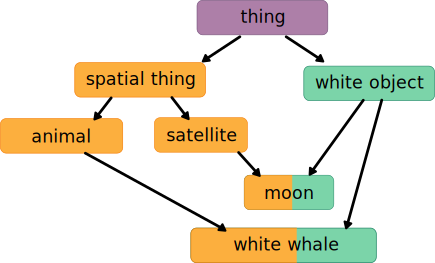
\includegraphics[width=0.7\columnwidth]{oroserver/commonancestors.pdf}
    \caption{Sample taxonomy to illustrate \emph{common ancestors} algorithms.}
    \label{fig|common-ancestors}
\end{figure}

\small
\begin{pseudocode}[ruled]{CommonAncestors}{concept1, concept2}
\label{algo|common-ancestors}

\BEGIN
\mathcal{I} \GETS \CALL{Superclasses}{concept1} \cap \CALL{Superclasses}{concept2} \\
\RETURN {c \in \mathcal{I} | \CALL{Subclasses}{c} \cap \mathcal{I} = \emptyset}\\
\END

\end{pseudocode}
\normalsize

Taking the taxonomy in figure~\ref{fig|common-ancestors} as example, the common
ancestors for the pair \concept{\{white whale, moon\}} are
\concept{\{spatial thing, white object\}}, \ie the set of classes that belong to
the intersection of the super-classes of both the concepts that have no
sub-classes in this intersection.

\small
\begin{pseudocode}[ruled]{FirstDifferentAncestors}{concept1, concept2}
\label{algo|first-different-ancestors}

\BEGIN
\mathcal{C} \GETS \CALL{CommonAncestors}{concept1, concept2} \\
\mathcal{S} \GETS \CALL{Superclasses}{concept1} \cup \CALL{Superclasses}{concept2} \\

\RETURN{\forall c \in \mathcal{C}, \CALL{DirectSubclasses}{c} \cap \mathcal{S}} \\
\END

\end{pseudocode}
\normalsize

The \emph{First Different Ancestors} algorithm
(algorithm~\ref{algo|first-different-ancestors}) returns the list of direct
sub-classes of the common ancestors. They are intuitively the most generic
types that \emph{differentiate} the two concepts. In the taxonomy
figure~\ref{fig|common-ancestors}, two instances \concept{a} and \concept{b} of
respectively \concept{white whale} and \concept{moon} have as first different
ancestors the two sets \concept{\{animal, satellite\}} (subclasses of ancestor
\concept{spatial thing}) and \concept{\{white whale, moon\}} (subclasses of
ancestor \concept{white object}).

\paragraph{Clarification Algorithm}
\label{sect|clarify}

During interactions with other agents, the robot is often required to figure
out which individual correspond to a description like ``red object'', ''a
bottle'', ''a book larger than this other one'', etc. This is a key part of the
grounding capability.

Clarification and discrimination algorithms are based on what we call
\emph{descriptors}: descriptors can be properties of individuals, either
acquired by the robot are statically asserted in a common-sense ontology. They
are also the result of other reasoning algorithms like the \emph{Common
Ancestors} and \emph{Different Ancestors} algorithms presented above.
We shall see later how symbolic knowledge is first acquired from geometric
reasoning or natural language processing, and we consider in this section that
the \emph{clarification} process is based on an established ontology, like the
sample proposed in figure~\ref{fig|discriminant}.

Based on all this information, and a given partial (or complete) description of
an object (list of attribute-value pairs), the robot is able to identify the
referred object the following way (Algorithm~\ref{algo|clarify}). First it
obtains all objects that fulfil the initial description. Based on the result
it either succeeds (obtains one single object), fails (no object with that
description could be found) or obtains several objects. In this latter case, a
new descriptor is added (mark~\ref{clar.desc}) to the initial description and
the process starts over again until all possible descriptors have been added.

Failure occurs in two cases: when the description does not match any object
from the robot's knowledge, either because the robot's knowledge is incomplete
(the human refers to an unknown descriptor or descriptor value) or due to
inconsistent information (human's and robot's beliefs differ), or when a set of
candidates could not get successfully discriminated with the available
descriptors.

In this latter case, new descriptors new be added (attribute-value pair). Two
alternatives are available: directly asking the human for a new descriptor, or
automatically searching a new attribute and ask the human for its value. In the
latter case, we need to automatically find the best discriminant for the
current list of objects being evaluated ($description$ in the algorithm).


\small
\begin{pseudocode}[ruled]{Clarify}{description}
\label{algo|clarify}
\BEGIN
candidates \GETS \CALL{GetObjectFromDescription}{description} \\
\IF \left|{candidates}\right| = 1 \THEN \RETURN{candidates[0]} \\
\ELSEIF \left|{candidates}\right| = 0 \THEN \OUTPUT{\mbox{No object found!}} \\
\ELSE
    \BEGIN
        description \GETS \CALL{AddDescriptor}{description} \STMTNUM{7em}{clar.desc}\\
        \RETURN{\CALL{Clarify}{description}} \\
    \END
\END

\end{pseudocode}
\normalsize

\paragraph{Finding a discriminant}
\label{sect|discriminant}

\begin{figure}
    \centering
    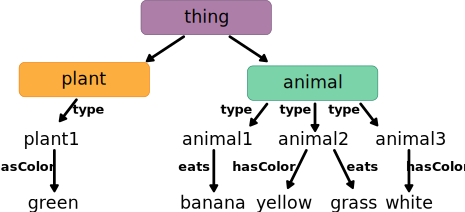
\includegraphics[width=0.7\columnwidth]{oroserver/discriminant.pdf}
    \caption{Sample ontology to illustrate the discrimination routines.
    \concept{plant1} is an instance of \concept{Plant} and
    \concept{animal[1-3]} are instances of \concept{Animal}.}
    \label{fig|discriminant}
\end{figure}

We have implemented a set of semantic categorisation functions in ORO. One of
them consists in looking for discriminants, \ie descriptors that allow a
maximum discrimination among a set of individuals. In the example above,
considering the attributes \emph{type, colour} and \emph{material}, ORO would
return \emph{colour} and \emph{material} as discriminants, since their values
are unique for the given set of objects.

We distinguish two types of discriminants. \emph{Complete} discriminants are
those attributes (or properties) that totally discriminate the set of
individuals. In other words, properties whose values can uniquely identify
those individuals. However, they are not always available. First, because two
or more individuals may share the same value, and second, because not all
individuals may share the same properties. Thus, \emph{partial} discriminants
are those that ``better'' split the set of individuals in different subsets
based on some criteria.

The algorithm to determine the type of discriminant available
(Algorithm~\ref{algo|discriminant}) has the following steps (to better follow
it, we base its description on the ontology example illustrated in
figure~\ref{fig|discriminant}. We search a discriminant for the following
individuals: \concept{plant1}, \concept{animal1}, \concept{animal2} and
\concept{animal3}. First we obtain the direct properties for all the
individuals, \ie we do not consider all the hierarchy of properties. In the
example, \concept{plant1} has two super-classes (\concept{Plant} and
\concept{Thing}), but we only take the most direct one (the class
\concept{Plant}). Next, we compute the number of individuals per property
(mark~\ref{disc.nbind}) and the number of different values for that property
(mark~\ref{disc.nbval}). If there is more than one different value for the
property (in other words, if not all individuals have the same value), then we
consider that property as a potential discriminant (mark~\ref{disc.append}).
Finally, we rank (mark~\ref{disc.rank}) the list of potential properties
following two criteria: the number of individual occurrences (\ie the most
individuals are covered by that property, the better) and the values
occurrences (\ie the more distinct values, the better).  The best discriminant
corresponds to the first element of the sorted list. In other words, the class
with higher number of occurrences and more variety in it.  If several
properties are equal, we return all of them.

In our example, the algorithm would return the class name as the partial
discriminant. If we only consider the instances of the class \concept{Animal},
it would return two properties equally discriminant: \concept{hasColor} and
\concept{eats}. It should be noted that this way of proceeding does not respect
the open world assumption. In this case, we believe that the robot should only
reason based on his current knowledge.

\small
\begin{pseudocode}[ruled]{GetDiscriminant}{individuals}
\label{algo|discriminant}
\BEGIN
P \GETS \CALL{Ontology.GetProperties}{individuals} \\
\hat{P} \GETS \emptyset \\
\FOREACH p \in P \DO
    \BEGIN
        n_{ind} \GETS \CALL{NbIndividualsWithProperty}{p} \STMTNUM{7em}{disc.nbind}\\
        n_{val} \GETS \CALL{NbDifferentValues}{p} \STMTNUM{10.9em}{disc.nbval}\\
        \IF n_{val} > 1 \THEN
            \hat{P} \GETS \CALL{Append}{[p,n_{ind},n_{val}]} \STMTNUM{8.8em}{disc.append}\\
    \END \\

\CALL{Rank}{\hat{P}} \STMTNUM{23.6em}{disc.rank}\\
\RETURN{\hat{P}[0][0]} \\
\END

\end{pseudocode}
\normalsize


\subsubsection{Memory}
\label{sect|oroserver-memory}

The ORO server offers a mechanism to mimic simple forms of biological memory.
When new statements are inserted in the knowledge base, a \emph{memory profile}
can be attached to this set.

Three such profiles are predefined: {\tt short term}, {\tt episodic} and {\tt
long term}. They each correspond to a different lifetime for the statements
(respectively 10 seconds, 5 minutes and no time limit). After this duration,
the statements are automatically removed from the knowledge base.

This approach is limited. In particular, \emph{episodic} memory primarily refers
to the semantics of the statements (that is expected to be related to an event)
and not to a specific life duration. We discuss at the end of this work possible
improvements.

\paragraph{Active Concepts} \emph{Short term} memory, however, is used in real
world applications, in particular to implement the idea of \emph{active
concept}: some modules, like our natural language processor (described later
on, at chapter~\ref{chapt|dialogs}), use the {\tt short term} memory profile to
mark for a few seconds important concepts that are currently manipulated by the
robot. For example, if a human asks the robot: ``Give me all red objects'', the
human, the \concept{Give} action, and each red objects that are found are
successively marked as \emph{active concepts} by inserting statements like
\stmt{human type ActiveConcept} in the short-term memory (which can be
considered, in this case, to be a working memory, as distinguished at
section~\ref{sect|memory}).


\subsubsection{Knowledge Structure Alteration and Learning}

In the ORO server, the knowledge structure (\emph{TBox}) is purely declarative
and asserted as regular statements (like \stmt{Location subClassOf
SpatialThing}), following the RDF Schema (RDFS) and OWL language constructs.
Table~\ref{table|main-tbox-properties} presents few of the main properties and
classes defined in RDFS and OWL that allow to describe the ontology
structure. These constructs can all be inserted at run-time to alter the
knowledge model of the server.

\begin{table}
\begin{center}

\begin{tabular}{ll}
\toprule
{\bf Name} & {\bf Example} \\
\midrule
{\tt rdfs:subClassOf} & \stmt{Human subClassOf Agent} \\
{\tt rdfs:subPropertyOf} & \stmt{hasColor subPropertyOf hasFeature} \\
{\tt rdfs:domain} & \stmt{thinks domain IntelligentAgent} \\
{\tt rdfs:range} & \stmt{name range string} \\
{\tt owl:inverseOf} & \stmt{sees inverseOf seenBy} \\
{\tt owl:FunctionalProperty} & \stmt{age type FunctionalProperty} \\
{\tt owl:TransitiveProperty} & \stmt{isAbove type TransitiveProperty} \\

\bottomrule

\end{tabular}
\end{center}

\caption{Some of the properties and classes defined in RDFS and OWL that allow
to define the semantics and relations of terms within an ontology.}

\label{table|main-tbox-properties}
\end{table}


We have not addressed the issue of learning in general in this work. However,
coupled with language processing features, the ability to easily alter the
knowledge structure allows for implementation of specific learning mechanisms.
For example, one can teach the robot that cats are animals by processing a
sentence like ``Cats are animals'' into \stmt{Cat subClassOf Animal} and then
adding it at run-time into the knowledge base. From that points, all entities
asserted or inferred to be cats will be as well inferred to be animals.

The case study \emph{Point \& Learn} (section~\ref{expe|pointandlearn})
presents some experimental results in this domain.

\subsubsection{Fast Concept Lookup}
\label{sect|oroserver-lookup}

Because this operation is frequent, in particular for language processing
application, the ORO server also provides a fast concept look-up mechanism to
search for a concept identifier by its human-friendly name (label) that takes
into account the language configuration.

%%%%%%%%%%%%%%%%%%%%%%%%%%%%%%%%%%%%%%%%%%%%%%%%%%%%%%%%%%%%%%%%%%%%%%%%%%%%%%
%%%%%%%%%%%%%%%%%%%%%%%%%%%%%%%%%%%%%%%%%%%%%%%%%%%%%%%%%%%%%%%%%%%%%%%%%%%%%%
%%%%%%%%%%%%%%%%%%%%%%%%%%%%%%%%%%%%%%%%%%%%%%%%%%%%%%%%%%%%%%%%%%%%%%%%%%%%%%

\section{Knowledge instantiation: the OpenRobots Common-Sense Ontology}

How much knowledge is available? Which content? How big is the knowledge base?

\subsection{Designing the \textsc{OpenRobots} common-sense ontology}
\label{sect|commonsense-design}

\begin{figure}
    \centering
    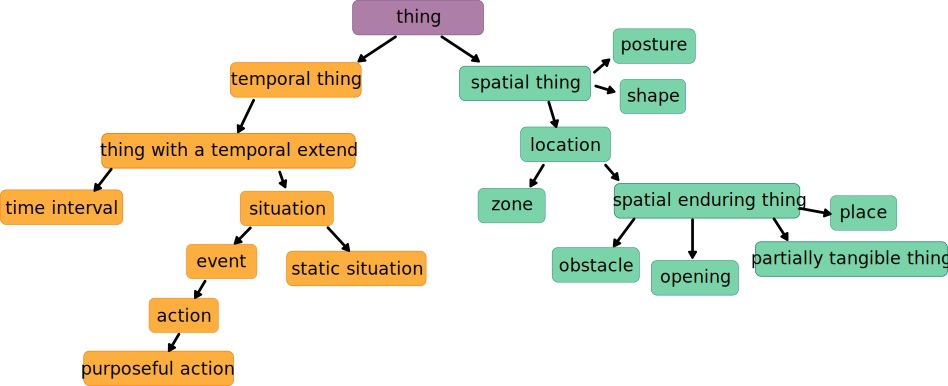
\includegraphics[scale=0.6]{oro/top_tbox.pdf}
    \caption{The upper part of the ORO common-sense TBox.}
    \label{fig|upper_tbox}
\end{figure}

\begin{figure}
    \centering
    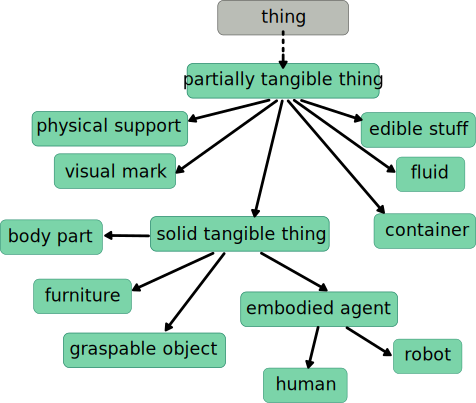
\includegraphics[scale=0.6]{oro/tangible_things_tbox.pdf}
    \caption{TBox of the specialisations of \concept{PartiallyTangible}.}
    \label{fig|tangible_things_tbox}
\end{figure}


\begin{table}
\begin{center}

\begin{tabular}{ll}
\toprule
Expressiveness & $\mathcal{SROIQ(D)}$ \\
Axioms & 961 (annotations: 359)\\
Class count & 108 \\
Object property count & 78 \\
Data property count & 13 \\
Individual count & 21 \\
Functional properties & 19 \\
Inverse properties & 9 \\
Transitive properties & 4 \\
Symmetric properties & 3 \\
\bottomrule

\end{tabular}
\end{center}

\caption{Statistics on the ORO common-sense ontology.}

\label{table|onto-stats}
\end{table}



\subsection{Internationalisation}
\label{sect|commonsense-i13n}

\chapter{Knowledge model and implementation}
\label{chapter|implementation}

\section{Knowledge model}
\label{sect|knowledge-model}

\subsection{OWL-DL ontologies}
\label{sect|owldl-ontologies}

\subsection{Parallel models}
\label{sect|parallel-models}

\subsection{Expressiveness}
\label{sect|expressiveness}

\section{ Architecture and core services}
\label{sect|oro-core}

\subsection{A server-based implementation}
\label{sect|oro-serverbased}

\section{Building an architecture on semantic events}
\label{sect|events}

\section{Inference techniques}
\label{sect|inference-techniques}

\subsection{Reasoning and inconsistency handling}
\label{sect|reasoning}

\subsection{Classification and discrimination}
\label{subssect|discrimination}

\subsection{Memory}
\label{subssect|memory}

\section{Interfacing}
\label{sect|interfacing}

\chapter{Knowledge Enabled Situated Natural Language Processing}
\label{chapt|dialogs}

%%%%%%%%%%%%%%%%%%%%%%%%%%%%%%%%%%%%%%

\fxwarning{Mention and detail immanent communication -> context sharing}

\section{Grounding verbal interaction into the robot knowledge}
\label{sect|dialogs}

\subsection{Situated speech acts}
\label{intro_example}

A messy table, covered with cardboard boxes, books, video tapes... Thomas is
moving and packs everything with the help of Jido, its robot.

`` -- Jido, give me this'', says Thomas, looking at a box that contains a video
tape. The robot smoothly grasps the tape, and hands it to the human.

While this kind of interaction should hopefully sound quite familiar in a
foreseeable future, our robots are not yet quite up to the task. Neither
regarding natural language understanding nor plan-making and manipulation.

To be combined together, those abilities require an unambiguous and shared
representation of concepts (objects, agents, actions...) underlying the
interaction: what are the prerequisites for such a
human sentence --- ``Jido, give me this'' --- to be understood by the robot,
correctly interpreted in the spatial context of the interaction, and ultimately
transformed into an action?

Austin~\cite{Austin1962} would have at first glance analysed such kind of
sentence as a \emph{speech act}, comprising of \emph{locutionary},
\emph{illocutionary} and possibly \emph{perlocutionary} acts. First, we want to
understand the direct meaning of the sentence (\emph{locutionary act}): we must
acquire the sentence, convert it into a useful syntactic form (quite probably
by mean of speech recognition), and understand the semantics of the sentence,
\ie, What is referred by ``\textit{Jido}''? What is ``\textit{give}''? What is
``\textit{me}''? And ``\textit{this}''?

Working in a situated context, we want furthermore to \emph{resolve} these
semantics atoms, \ie ground them in the sensory-motor space of the robot. For
instance, ``\textit{this}'' is a demonstrative pronoun that refers in this
context to the object the human is focusing on, whatever \textit{focusing}
means: here, Thomas is looking at something, which is a possible cue. But it
could as well point at something or refer to some previously mentioned concept. 

\begin{figure}%[!ht] 
	\centering
	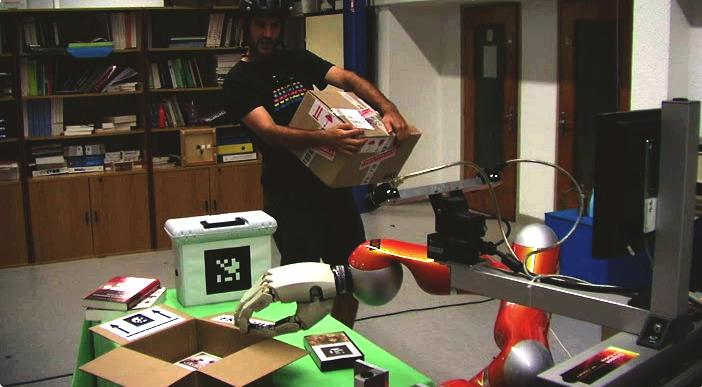
\includegraphics[width=0.9\linewidth]{images/dialogs/pt.jpg} 
	\caption{Interacting with
	the robot in an everyday setup: the human asks for help in vague terms, the
	robot takes into account the human's spatial perspective to refine its
	understanding of the question.} 
	\label{fig|vpt} 
\end{figure}


Second, the \emph{illocutionary force}, \ie the \emph{intent} of the utterance
as thought by the agent must be extracted, and understood. In our example,
Thomas obviously wants an action to be performed by the robot. The action
parametrisation is conveyed by the semantics attached to the words and the
grammatical structures of the sentence. In our example, the type of action is
given by the verb ``\textit{give}''. Assuming the robot has some procedural
knowledge attached to this symbol, the action type can be considered as
grounded for the robot. We can as well understand that the recipient of the
action is the human, the performer is the robot itself, and the object acted
upon is the tape. These are the basic \emph{thematic roles}~\cite{Gruber1965}
that can be extracted from the sentence that allow to fully ground the action.

\subsection{Building a symbolic model}

Extracting these speech acts and turning them into a content processable by the
robot is a difficult challenge in the general case. We base our approach on
three distinct, inter-related cognitive functions:

\begin{inparaenum}[\itshape 1)]

\item \emph{Physical environment modelling} and \emph{spatial reasoning}
(grouped under the term \emph{situation
assessment})  are in charge of building and
maintaining a coherent model of the physical world. This model is realistic in
the sense that it relies on accurate 3D models of both manipulated objects and
humans. It also has dedicated mechanisms to manage disappearing or occluded
objects.  The geometric model is used to compute several spatial properties of
the scene that actually convert the original sensory data into symbolic
beliefs. This includes relative locations of objects, visibility state,
gestures like pointing, etc.  Assuming that other agents are as well
represented in the model, the same computations are applied to analyse the
scene from each agents' point of view (\ie from their \emph{perspectives}).
This approach is presented in depth in~\cite{Sisbot2011}.

\item \emph{Knowledge representation and management}: the robot is endowed with
an active knowledge base that provides a logically sound symbolic model of its
beliefs on the world, as well as models for each cognitive agent the robot
interacts with. Each of these models is independent and logically consistent.
This enable reasoning on different perspectives of the world that would be
considered otherwise inconsistent (for instance, an object can be visible for
the robot but not for the human. This object can have at the same time the
property {\tt isVisible \textbf{true}} and {\tt isVisible \textbf{false}}, in
two different models).  Our platform also features continuous storage, querying
and event triggering over the pool of facts known by the robot. It relies on
OWL ontologies (a decidable subset of the predicate logics). The knowledge base
is presented in~\cite{Lemaignan2010}.

Used in combination with the situation assessment framework, the robot is thus
able to maintain different models of the world, one per agent. This proves an
essential feature (\cite{Roy2005, Kruijff2010}) to enable perspective-aware
grounding of natural language, as we will see in next sections.

\item \emph{Dialogue input processing}, including natural language parsing
capabilities, disambiguation routines and interactive concept anchoring. We
focused our efforts on three classes of utterance, commonly found in
human-robot interaction: \emph{statements} (\ie new facts the human wants to
inform the robot), \emph{orders} (or more generically \emph{desires}) and
\emph{questions on declarative knowledge} (whose answers do not require
explicit planning). This would roughly cover the \emph{representative}
(sometimes referred as \emph{assertives}) and \emph{directives} type of
illocutionary acts, in Searle~\cite{Searle1976} classification. This paper
focuses on this last facet (dialogue processing).

\end{inparaenum}

\subsection{Related work}

Processing natural language in situated context is already an established
research field. In~\cite{Roy2005}, Roy summarises what he sees as the main
challenges to be tackled: cross-modal representation systems, association of
words with perceptual and action categories, modelling of context, figuring out
the right granularity of models, integrating temporal modelling and planning,
the ability to match past (learned) experiences with the current interaction
and the ability to take into account the human perspective.

Kruijff et al. provides in~\cite{Kruijff2010} an up-to-date survey of literature
on situated human-robot dialogue, focusing on formal representation systems,
bi-directionality of the interaction and context building. They point as well
that, compared to the cognitive psychology community, the ``situated AI''
community started only recently to take into account agents focus, perspective and temporal
projection abilities.

Dialogue processing on real robots have been explored by several teams.
Scheutz~\cite{Brick2007} has contributions regarding natural language
processing in an incremental way, and how this enables instant back-channel
feedback (like nodding).

Hüwel et al.~\cite{Huwel2006} propose the concept of \textit{Situated Semantic
Unit}: these meaning atoms are extracted from sentences and expose semantic
links to other units. The parser tries to satisfy these links and rate
accordingly the semantic interpretation of the sentence. Used in conjunction
with ontologies, their approach offers good robustness to ungrammatical or
partial utterances. They validated the approach with an extensive user-study.

\fxwarning{Kollar/Tellex}

Also worth mentioning, Mavridis and Roy~\cite{Mavridis2005} propose the idea of
a \emph{grounded situation model} which is an amodal model of the world where
different sensing modalities, including verbal ones (the robot is able to
\emph{imagine} objects), are merged. Their framework also allows management of
the interaction history (the human can ask for a past event). They propose an
implementation in an environment built on simple entities (a manipulator arm
and colour balls).

\subsection{Contribution}

Compared to previous contributions, our efforts have two foci: {\it (1)}
integration between language processing and perception of the environment and
the humans, from several perspectives; and {\it (2)} realistic human-robot interactions:
real-time processing; open speech; complex, dynamic, partially unknown human environments; fully
embodied autonomous robots with manipulation abilities. 

We do not claim any contribution to the field of computational linguists (see
\cite{Kruijff2010} for a survey of formal approaches to natural language
processing in the robotics field): our main contribution here is the grounding
of concepts involved in the human discourse through the robot's own knowledge.

Section~\ref{dialog} presents the overall grounding process, section~\ref{examples} 
proposes an analysis of the processing of three prototypical sentences. 
Experimental results are presented in section~\ref{experiment}. A 
discussion regarding the current limitations of our system concludes
this article.

%%%%%%%%%%%%%%%%%%%%%%%%%%%%%%%%%%%%%
\section{The Natural Language Grounding Process}
\label{dialog}

Verbal interaction with human presents two categories of challenges: syntactic
ones, and semantic ones. The robot must be able to process and analyse the
structure of human utterances, \ie natural language sentences, and then make
sense of them. As stated in the introduction, we process three categories of
sentences: \emph{statements}, \emph{desires} and \emph{questions} that can be
answered from the declarative knowledge present in the robot knowledge base (a
choice similar to the \emph{Behaviour Cycle} in the GLAIR
architecture~\cite{Shapiro2009}). In our work, the grounding process of the
human discourse consists in extracting either the \emph{informational} content
of the sentence to produce statements or its \emph{intentional} content (\ie
performative value) to collect orders and questions. We do not claim any
contribution to the field of computational linguists (see \cite{Kruijff2010}
for a survey of formal approaches to natural language processing in the
robotics field). Our main contribution here is the grounding (we call it
\emph{resolution}) of concepts involved in the human discourse through the
robot's own knowledge.

We have developed a dedicated module called {\sc
Dialogs}\footnote{\textsc{Dialogs} is an open-source project. Source code is
available from \url{http://dialogs.openrobots.org}.} that processes human
input in natural language, grounds the concepts in the robot's knowledge and
eventually translates the discourse in a set of declarative OWL/RDF statements.

\begin{figure}[!ht]
\centering
  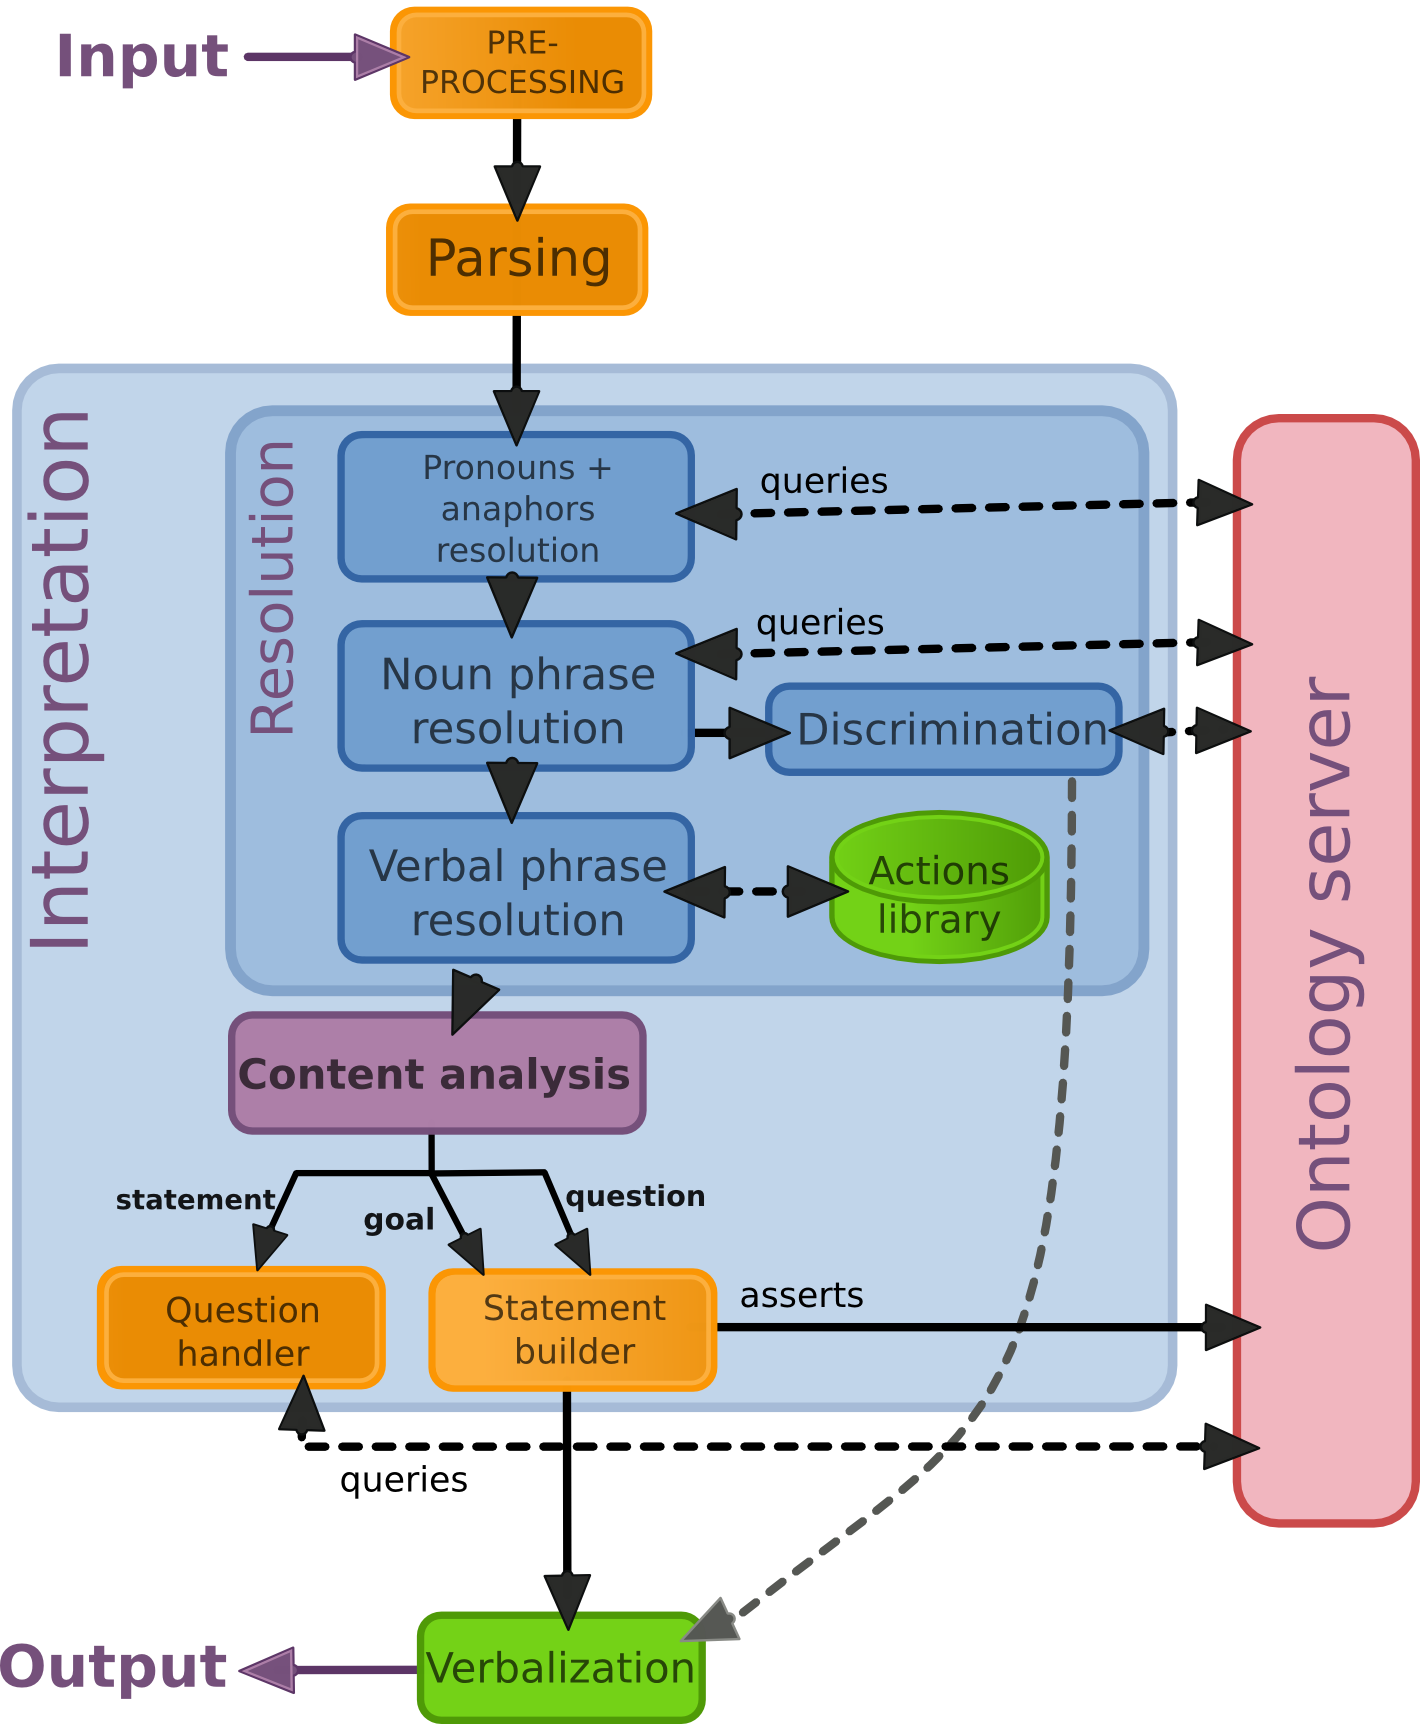
\includegraphics[width=0.6\linewidth]{images/dialogs/dialog_module_simple.pdf}
  \caption{The {\sc Dialogs} module has three main steps: the parsing,
  the interpretation and the verbalisation. The interpretation module is
  responsible for both the \emph{resolution} and the semantic content
  \emph{analysis and translation}.} 
  \label{fig|dialog}
\end{figure}

As shown in Figure~\ref{fig|dialog}, the {\sc Dialogs} module is composed of
three main blocks. The user's input is first pre-processed. For instance,
\emph{I'm} constructs are expanded into \emph{I am} and then parsed. The parser
is a custom-made, rule-based (\ie grammar-free) tool that extracts the
grammatical structure from the user's sentence.

Figure~\ref{dialog|parser_output} shows an example of the raw output of the
parser for a moderately complex sentence.

\begin{figure}%[!ht]
\begin{center}
\scriptsize
\begin{alltt}
>> IMPERATIVE
VP: \textbf{remember} (present simple)
    SUBSENTENCE (aim: that)
      NP: \textbf{I}
      VP: \textbf{want} (present simple)
        direct objects: 
          NP: \textbf{you}
        secondary VP: \textbf{give} ()
              direct objects:
                NP: my \emph{nice blue} \textbf{bottle}
              indirect objects:
                NP: \textbf{me}
\end{alltt}
\end{center}
\caption{Raw output of the {\sc Dialogs} parser after processing the
sentence: ``remember that I want you to give me my nice blue bottle.'' 
Nominal groups are not grounded yet.} 
\label{dialog|parser_output}
\end{figure}

The result of the parsing is then sent to the \emph{interpretation} module, the
core of the approach.  Interpretation consists in three distinct operations:
the sentence \emph{resolution} (concepts grounding), the \emph{content
analysis} (what is the intent of the utterance: information, question or
desire) and the \emph{statement building} (translation into RDF statements).

The sentence resolution has three steps: {\it(1)} pronouns and anaphora are
replaced by, respectively, the correct speaker ID and the ID of the last object
spoken about (extracted from the dialogue history), {\it(2)} nominal groups are
disambiguated and grounded (noun phrase resolution), and {\it(3)} verbal groups
are resolved as well, and their associated thematic roles are retrieved (verbal
phrase resolution). Algorithm~\ref{algo|Resolution} describes the overall
process.  Next section describes specific examples to show how the noun and
verbal phrase resolution takes place.

\small
\begin{pseudocode}[ruled]{Resolution}{sentence, currentSpeaker}
\label{algo|Resolution}

\mathcal{G} \GETS \CALL{ParseNominalGroups}{sentence} \\

\FOREACH g \in \mathcal{G} \DO 
\BEGIN
   \mathcal{D} \GETS \CALL{GenerateDescription}{g} \STMTNUM{5.1em}{res.desc}\\
   candidates \GETS \CALL{Ontology.Find}{\mathcal{D}} \STMTNUM{4em}{res.onto}\\
   
   \IF \left|{candidates}\right| = 0 \THEN
    \BEGIN
      \OUTPUT{\mbox{Couldn't resolve the group!}} \\
      \EXIT \\
    \END
   \ELSEIF \left|{candidates}\right| = 1 \THEN
      id \GETS candidates[0] \STMTNUM{8em}{res.easy}\\

   \ELSE
      \BEGIN
        \IF \CALL{Ontology.CheckEquivalent}{candidates} \THEN
          id \GETS candidates[0] \\
        \ELSE
          id \GETS \CALL{Discrimination}{candidates} \\ %\STMTNUM{1em}{st.discrimination}\\
      \END \\
   \CALL{Replace}{g, id, sentence}
\END
\end{pseudocode}
\normalsize

As represented in Figure~\ref{fig|dialog}, interpretation tightly relies on the
communication with the knowledge base. All the concepts the robot manipulates
are stored in the ontology server and retrieved through logical
queries, except for the verbs that are currently stored in a dedicated library
(the \emph{action library} in the diagram).

%%%%%%%%%%%%%%%%%%%%%%%%%%%%%%%%%%%%%
\section{Technical analysis}
\label{examples}

In order to better understand the overall process of the {\sc Dialogs} module
and its relation with ORO, we next describe the different steps of the approach
based on three examples. In these examples we assume that some initial facts
are present in the knowledge base (section~\ref{modeling_real_world} discusses
how the initial knowledge can be acquired), both in the robot's own model and
in the human's model.  Since the robot tries to ground a human utterance, all
queries are sent to the human model in order to interpret it from the human
perspective.

\subsection{Informational Content Extraction}
\label{informational_content_extraction}

\begin{figure}
    \centering
%	\begin{tabular}{p{0.5\columnwidth} | p{0.5\columnwidth}}}
	\begin{tabular}{l|l}
	\emph{Initial knowledge} \texttt{human\_01} &
	\emph{Human input}\\	
	
	\hline

    	\stmt{banana\_01 type Banana} &
	``The yellow banana is big!'' \\
	
    	\stmt{banana\_01 hasColor yellow} & \\
	\vspace{0.5em}\\
	\hline

	\emph{Generated partial statements} &
	\emph{Newly created statements}\\
	\hline

	\stmt{?obj type Banana} &
	\hspace{0.2cm}\stmt{banana\_01 hasSize big} \\
	
    	\stmt{?obj hasColor yellow} & \\
    	\hspace{0.2cm}$\Rightarrow$ \concept{?obj = banana\_01}\\

	\hline
	\end{tabular}
\caption{First example: content extraction.
``$\Rightarrow$'' represents the output of the ontology server.}
\label{dialog|ex1}
\end{figure}


Figure~\ref{dialog|ex1} shows a first example of human discourse grounding and
the extraction of informational content. We assume that the robot knowledge
base only contains two initial statements in the human model. The user asserts
a new one: ``The yellow banana is big!''.  We first want to match the nominal
group \emph{The yellow banana} to an already known concept
(algorithm~\ref{algo|Resolution}), and second to translate the property
\emph{is big} into a predicate ({\tt hasSize}) to state its semantics.


\small
\begin{pseudocode}[ruled]{GenerateDescription}{group}
\label{algo|GenerateDescription}

\PROCEDURE{GenerateDescription}{group} 
   noun \GETS \CALL{GetNoun}{group} \\ 
   \IF \CALL{Ontology.Lookup}{noun} \in (Instances) \STMTNUM{7.5em}{st.lookup} \THEN
   		\BEGIN
		id \GETS \CALL{Ontology.lookup}{noun}\\	
		\RETURN {\mathcal{D} + \{ *\ {\tt sameAs}\ <id> \}}\\
		\END
   \ELSE
    	\mathcal{D} = \mathcal{D} + \{ *\ {\tt type}\ <noun>\} \\
   
   \\
   det \GETS \CALL{GetDeterminant}{group} \\
   \IF det \in {\mbox(possessives)} \THEN
       \mathcal{D} = \mathcal{D} + \{ *\ {\tt isRelatedTo}\ <possessor>\} \\
    
    \IF det \in {\mbox(demonstratives)} \THEN
        \BEGIN
        \IF \CALL{Ontology.Check}{\{<currentSpeaker>\ {\tt focusesOn}\ *\}} \THEN 
            \mathcal{D} = \mathcal{D} + \{<currentSpeaker>\ {\tt focusesOn}\ *\}
        \ELSE
            \mathcal{D} = \mathcal{D} + \CALL{AnaphoricMatching}{} \STMTNUM{4em}{st.anaphoric} \\
        \END \\
   \\
   adjs \GETS \CALL{GetAdjectives}{group} \\
   \FOREACH adj \in adjs \DO
   	\BEGIN
   		\IF adj == <other> \THEN 
   			\BEGIN
   			id \GETS \CALL{History.GetMatchingGroup}{group} \STMTNUM{8em}{st.history}\\
   			\mathcal{D} = \mathcal{D} + \{ *\ {\tt differentFrom}\ <id> \}\\
   			\RETURN{D}\\
			\END   		
   		\ELSE
	     	\mathcal{D} = \mathcal{D} + \{ *\ {\tt hasFeature}\ <adj>\} \STMTNUM{9em}{st.adj} \\
    \END\\
    
   \\  
   nounComplements \GETS \CALL{GetNounComplements}{group} \\
   \FOREACH nouncmpl \in nounComplements \DO
     \mathcal{D} = \mathcal{D} + {\CALL{GenerateDescription}{nouncmpl}}\\
   
   
   \\  
   relativeClauses \GETS \CALL{GetSubordinateRelativeClauses}{group} \\
   \FOREACH relative \in relativeClauses \DO
   	\BEGIN
   	 \mathcal{G} \GETS \CALL{GetNominalGroups}{relative} \\
   	 \FOREACH g \in \mathcal{G} \DO
     	\mathcal{D} = \mathcal{D} + {\CALL{GenerateDescription}{g}}
    \END\\
     
   \\
   \RETURN{\mathcal{D}} 
\ENDPROCEDURE
\end{pseudocode}
\normalsize

\small
\begin{pseudocode}[ruled]{History.GetMatchingGroup}{group}
\label{algo|History}
\PROCEDURE{History.GetMatchingGroup}{group}
\COMMENT{Extract Nominal group from sentences stored in the history}\\
\mathcal{H} \GETS \CALL{History.GetAllNominalGoup}{}\\
\COMMENT{Generate description of the nominal group that is being processed.} \\
\COMMENT{The adjective  "other" is to be removed before calling this routine} \\
	\mathcal{G} \GETS \CALL{GenerateDescription}{group} \\ 
	
	candidates \GETS \mathcal{H} \cap \mathcal{G}\\
	\IF \left|{candidates}\right| = 0 \THEN
    \BEGIN
      \OUTPUT{\mbox{Couldn't find another object with the same characteristics!}} \\
      \EXIT \\
    \END
   \ELSEIF \left|{candidates}\right| = 1 \THEN
      id \GETS candidates[0]
   \ELSE
   	  id \GETS \CALL{Discrimination}{candidates}\\
   \RETURN{id}
\ENDPROCEDURE
\end{pseudocode}
\normalsize

To resolve the nominal group \emph{The yellow banana} a set of partial
statements that describe the concept is generated based on the grammatical
parsing of the sentence (algorithm~\ref{algo|Resolution}(\ref{res.desc})). The
parsed tree of each nominal group is translated into statements based on a set
of rules.  In the example, a banana (\stmt{?obj type Banana}) that is yellow
(\stmt{?obj hasColor yellow})\footnote{Predicates like \concept{hasColor} or
\concept{hasSize} that bind \concept{banana\_01} to adjectives are extracted
from a predefined database of $[Predicate \rightarrow AdjectiveCategory]$, and
falls back on the generic \concept{hasFeature} predicate if the adjective is
not known.}.  Based on these partial statements a SPARQL query is sent to the
ontology server to retrieve possible instances that match the description
(algorithm~\ref{algo|Resolution}(\ref{res.onto})).

In this first simple case, the concept \concept{banana\_01} is unambiguously
matched (since there is only one possible banana) and returned. Finally, we can
now add the new information provided by the human, \ie the new statement
\stmt{banana\_01 hasSize big}, to the human model in the ontology server.

The translation of \emph{yellow} to \concept{hasColor yellow} is not obvious: in
the general case, we associate a adjective to the noun it characterises with
the \concept{hasFeature} predicate (for instance, \emph{The sight is beautiful}
would translate to \stmt{sight hasFeature beautiful}). But we can also manually
set the predicate associated to a category of adjectives: It is what has been
done for the main colours. Another example is the size: for known size
adjectives (big, small, etc.), the \concept{hasSize} predicate is being used.


\subsection{Intentional Content Through Verb Resolution}

The sentence in the first example is built with the state verb \emph{be} at
indicative. Let us examine a different example with an action verb at
imperative mode (an order): ``Give me the banana". The process is described in
Figure~\ref{dialog|ex2}.

\begin{figure}
    \centering
	\begin{tabular}{l|l}
	\emph{Initial knowledge} \texttt{human\_01} &
	\emph{Human input}\\
	
	\hline
	
    	\stmt{banana\_01 type Banana} &
	``Give me the banana.'' \\
	
    	\stmt{banana\_01 hasColor yellow} & \\
	\vspace{0.5em}\\
	\hline
    	
	\emph{Generated partial statements} &
	\emph{Newly created statements}\\
	\hline
    	\stmt{?obj type Banana} & 
	\stmt{human\_01 desires sit\_a3} \\
	
	\hspace{0.2cm}$\Rightarrow$ \concept{?obj = banana\_01}
    	& \stmt{sit\_a3 performedBy myself} \\
    	& \stmt{sit\_a3 actsOnObject banana\_01} \\
    	& \stmt{sit\_a3 receivedBy human\_01} \\
	\end{tabular}

\caption{Second example: processing an order.}
\label{dialog|ex2}
\end{figure}

\label{processing_of_actions}

In order to capture the intentional content of a sentence (for example, an
order) we need to retain the semantics of the verb and its complements.
\emph{Thematic roles} allow for semantically linking a verb to its complements.
There is no general agreement amongst linguists on a comprehensive list of
thematic roles. The amount and the granularity of roles varies a lot in the
literature~\cite{Gutierrez2001}. We thus use a small set of them, which matches
the relations the robot can actually achieve (we discuss possible extensions in
the conclusion). For instance, in the second example, the verb \emph{give} has
three thematic roles: \concept{performedBy}, \concept{actsOnObject} and
\concept{receivedBy}.

\begin{table}
\begin{center}
\begin{tabular}{lllll}
\toprule
{\bf Verb} & {\bf Grammatical Role} & {\bf Thematic Role} & {\bf Predicate} & {\bf Range} \\
\midrule
\multirow{2}{0.7cm}{\bf get} & Subject & Agent & \concept{performedBy} & \concept{Agent} \\
 & Direct object & Theme & \concept{actsOnObject} & \concept{Artifact} \\
\midrule
\multirow{3}{0.7cm}{\bf put} & Subject & Agent & \concept{performedBy} & \concept{Agent} \\
 & Direct object & Theme & \concept{actsOnObject} & \concept{Artifact} \\
 & Indirect object & Recipient & \concept{receivedBy} & \concept{PhysicalSupport} \\
\midrule
\multirow{3}{0.7cm}{\bf give} & Subject & Agent & \concept{performedBy} & \concept{Agent} \\
 & Direct object & Theme & \concept{actsOnObject} & \concept{Artifact} \\
 & Indirect object & Recipient & \concept{receivedBy} & \concept{Agent} \\
\midrule
\multirow{3}{0.7cm}{\bf move} & Subject & Agent & \concept{performedBy} & \concept{Agent} \\
 & \emph{Direct object} & \emph{Theme} & \concept{actsOnObject} & \concept{Artifact} \\
 & Indirect object & Goal & \concept{hasGoal} & \concept{Location} \\
\midrule
\multirow{3}{0.7cm}{\bf show} & Subject & Agent & \concept{performedBy} & \concept{Agent} \\
 & Direct object & Theme & \concept{actsOnObject} & \concept{Location} \\
 & \emph{Indirect object} & \emph{Recipient} & \concept{receivedBy} & \concept{Agent} \\
\midrule
\multirow{2}{0.7cm}{\bf look} & Subject & Agent & \concept{performedBy} & \concept{Agent} \\
 & Indirect object & Goal & \concept{hasGoal} & \concept{Location} \\

\bottomrule

\end{tabular}
\end{center}
\caption{Main action verbs known to {\sc Dialogs} and associated thematic
roles. Italics denotes optional roles.}
\label{table|thematic-roles}
\end{table}

The list of actions the robot can plan for (currently \emph{take},
\emph{place}, \emph{give}, \emph{show}, \emph{hide} and \emph{move}) along with
possible synonyms (for example, \emph{to pick} and \emph{to take} are set as synonyms of \emph{to
get}) and their associated thematic roles are stored in a predefined library
of actions (table~\ref{table|thematic-roles} and figure~\ref{fig|dialog}).
For each action we identify and store: the role of the subject in
the sentence (always \concept{performedBy}); the role of the direct object (for
instance, \concept{actsOnObject}); and the role of each of the indirect objects
with their optional prepositions (for instance,
\concept{receivedBy})\footnote{Note that in example 2, ``give me the banana'',
the pronoun ``me'' appears before ``banana'', while it is an indirect
complement --- ``give it {\bf to me}''. The parser correctly handles these
cases.}. Moreover, through the ontology we check that each holder of a role is
semantically consistent. For instance, the action \emph{Give} must have a
manipulable physical item (\concept{Artifact}) as direct object. Thus, if the
concept the robot finds for the thematic role \concept{actsOnObject} cannot be
inferred to be an artifact, the robot goes back to the human saying it does not
understand.

This second example  also shows the pronoun reference resolution: ``me'' is
replaced by the id of the current speaker, while ``you'' is replaced by
\concept{myself} (\concept{myself} always represents the robot itself). When
present, anaphoras (references to previous concepts like ``give me the banana,
I like {\bf it}.'') are also resolved in the same step.

Once the sentence is completely resolved and translated into a formal
representation (a human desire in this example\footnote{Orders are here
represented as human desires: the human desires a specific new situation.}), we
store it in the ontology server. The robot's decisional/executive layers can
then decide whether to execute the order or not. 

\subsection{Informational Content Extraction Requiring Clarification}
\label{dialogs:disamb}
\begin{figure}
    \centering
	\begin{tabular}{p{7cm}}
	\emph{Initial knowledge model of} \texttt{human\_01}\\
	\hline
     	\hspace{0.3cm}\stmt{banana\_01 type Banana} \\
     	\hspace{0.3cm}\stmt{banana\_01 hasColor yellow} \\
     	\hspace{0.3cm}\stmt{banana\_02 type Banana} \\
     	\hspace{0.3cm}\stmt{banana\_02 hasColor green} \\
	\end{tabular} \\

	\vspace{0.5em}

	\begin{tabular}{p{7cm}}
	\emph{Human input}\\
	\hline
     	\hspace{0.3cm}``The banana is good.'' \\
	\end{tabular} \\

	\vspace{0.5em}

	\begin{tabular}{p{7cm}}
	\emph{Generated partial statements}\\
	\hline
     	\hspace{0.3cm}\stmt{?obj type Banana} \\
	\hspace{0.7cm} $\Rightarrow$ \concept{?obj = [banana\_01, banana\_02]}
	\end{tabular} \\

	\vspace{0.5em}

	\begin{tabular}{p{7cm}}
	\emph{Discrimination process}\\
	\hline
     	\hspace{0.3cm}\concept{discriminate([banana\_01, banana\_02])} \\
	\hspace{0.7cm} $\Rightarrow$ \concept{?hasColor = [yellow, green]}
	\end{tabular} \\

	\vspace{0.5em}

	\begin{tabular}{p{7cm}}
	\emph{Robot output speech}\\
	\hline
     	\hspace{0.3cm}``The yellow one or the green one?'' \\
	\end{tabular} \\

	\vspace{0.5em}

	\begin{tabular}{p{7cm}}
	\emph{Human answer}\\
	\hline
     	\hspace{0.3cm}``The green one.'' \\
	\end{tabular} \\
    
	\vspace{0.5em}

	\begin{tabular}{p{7cm}}
	\emph{Extended human input}\\
	\hline
     	\hspace{0.3cm}``The green banana is good.'' \\
	\end{tabular} \\
	
	\vspace{0.5em}

	\begin{tabular}{p{7cm}}
	\emph{Generated partial statements}\\
	\hline
     	\hspace{0.3cm}\stmt{?obj type Banana} \\
     	\hspace{0.3cm}\stmt{?obj hasColor green} \\
	\hspace{0.7cm} $\Rightarrow$ \concept{?obj = [banana\_02]}
	\end{tabular} \\
    
	\vspace{0.5em}
	\begin{tabular}{p{7cm}}
	\emph{Newly created statements}\\
	\hline
     	\hspace{0.3cm}\stmt{banana\_02 hasFeature good} \\
	\end{tabular}

\caption{Ambiguity resolution: in this example, ``banana'' can refer to the
yellow banana (\concept{banana\_01}) or the green one (\concept{banana\_02}).
Discrimination routines handle the disambiguation process.} \label{dialog|ex3}
\end{figure}

This last example (Figure~\ref{dialog|ex3}) shows the resolution of ambiguous
concepts. In this case the user refers to ``the banana'' while two instances of
the \concept{Banana} class exist in the ontology. The robot needs to find out
to which instance the user is actually referring to. To this end,
disambiguation routines
(algorithm~\ref{algo|Resolution}(\ref{st.discrimination})~\cite{Ros2010b}
\fxwarning{add a link to appropriate section} find differences between the
instances (in the example, one banana is yellow while the other one is green)
and build a sentence through the \emph{verbalisation} module to ask the user a
closed question that will help clarify the ambiguity: ``Is it yellow or
green?'' The user's answer is parsed and merged with the previous sentence. The
resulting, augmented, sentence (``The green banana is good") goes again through
all the interpretation steps. This process is repeated until no ambiguities
arise.  In the example, the \concept{banana\_02} is finally returned.

If no differences \fxfatal{should we say 'in the human model', even if 
getDiscriminantForAgent currently doesn't work?} can be found, an open question 
(``give me more information'') is send to the human.

Several other strategies are used in parallel to disambiguate concepts without
having to ask for more information to the human:

\begin{itemize}
	\item Which objects are currently visible to the human? If only one of
	them, then it is probably the one the user is talking about. 
	\item Did a previous interaction involved a specific object that would
	still be the subject of the current sentence?
	\item Is the user looking or pointing at a specific object?
\end{itemize}

Two cases can alter the way the discrimination routines work:
\begin{enumerate}
    \item If a sentence starts with {\it Learn that...}, failures during 
    discrimination are interpreted as new concepts, and instead of marking the 
    nominal as not resolved, and new identifier is created and add to the knowledge base.
    \item For questions like {\it Which colour is the bottle?}, the discrimination 
    algorithm can not use the feature {\it colour} to identify to bottle. The 
    resolution algorithm pass this kind of constraints as a parameter of the 
    discrimination routines.
\end{enumerate}

 
While no examples involving questions have been detailed, factual \emph{wh-}
questions and polar (\emph{yes/no}) questions can be processed in a similar way
by \textsc{Dialogs}. For instance, a question like ``What is on the table?'' is
grounded (to extract the relation \concept{isOn} and to find what \emph{table}
refers to) and transformed into the following kind of query: \concept{find ?var
[\stmt{?var isOn table1}]}.  Answers are converted back to a full sentence by
the \emph{verbalisation} module, and uttered to the human.


The next chapter (page~\pageref{chapter|evaluation}) presents several
experiments that make intensive use of the {\tt Dialogs} module.


\chapter{Evaluation}
\label{chapter|evaluation}

\section{Comparison of oro-server with other existing systems}
\label{sect|evaluation-oroserver}

\subsection{Performances Analysis}

\section{Experimental evaluation}
\label{sect|experimental-evaluation}

Experimental validation of our work takes several forms that are presented in
this section.

First, it must be noted that our experiments are largely independant from the
underlying platform. Since our contributions are mainly at the symbolic
reasoning level, we rely on intermediate layers for the back and forth
conversion of sensori-motor data to symbols. These intermediate layers are
obviously much more dependant on the platform.

We present here three distinct experimental frameworks: first, we present the
MORSE simulator (section~\ref{sect|simulation}) that has been developed during
the thesis preparation with several features dedicated to human-robot
interaction simulation.

Then, several more ``traditional'' experiments on different robotic platforms
are presented (sections~\ref{sect|casestudies}, \ref{sect|expe1}
and~\ref{sect|expe2}). Most of these experiments have been conducted at
LAAS-CNRS and in other laboratories involved in the European CHRIS project
(\emph{Jido}, \emph{PR2}, \emph{ICub} and \emph{Bert} platforms).  Experiments
have also been conducted at Munich's IAS laboratory on the \emph{Rosie}
platform.

Finally, we report in section~\ref{sect|roboscopie} on the theater performance
\emph{Roboscopie} that was presented in 2011 at a large general public audience
in Toulouse.

\subsection{Simulation of HRI interaction}
\label{sect|simulation}

\subsubsection{The MORSE simulator}

The Modular OpenRobots Simulation Engine (MORSE)~\cite{Echeverria2011}
(figure~\ref{fig|morse-gui}) is a open-source tool developed for robotics
research. It is a domain independent simulator, where virtual robots can
interact with a 3D environment, using sensors and actuators that behave in the
same way as their counterparts in the real world.  MORSE relies on the advanced
3D (OpenGL shaders) and physics simulation ({\sc Bullet} physics engine)
capabilities of the Blender \emph{Game Engine}, a real-time 3D runtime
integrated to the open-source Blender modeling toolkit.  This allows for
semi-realistic simulation of complex environments.

\begin{figure}[t]
      \centering
      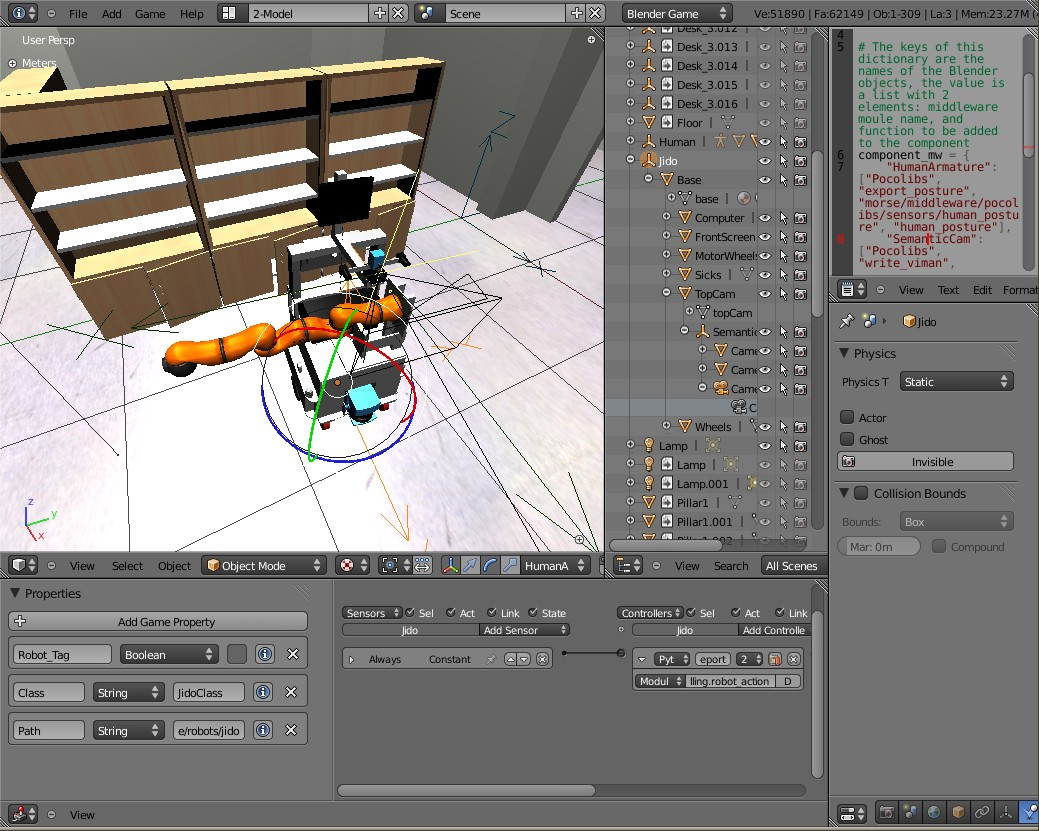
\includegraphics[width=0.7\columnwidth]{experiments/morse-interface.jpg}
      \caption{Screenshot of the MORSE graphical interface (inside Blender).}
      \label{fig|morse-gui}
\end{figure}


The MORSE components (sensors and actuators) exchange data with the robotics
software via middleware bindings, using a \emph{Software In The Loop} (SAIL)
architecture. Middleware supported in the current version include LAAS'
Pocolibs library, ROS and YARP, as well as a socket-based raw protocol. This
design allows in principle to use the same software in both the real robots and
the simulator. Instructions given to the robot are interpreted in the simulator
to provide the control of actuators, such as the motion of the robot and its
arms.  The data from simulated sensors is sent back through the middlewares,
{\it e.g.}~exporting the images from cameras, or the positions of the robot,
human and other objects of interest.

MORSE provides support for several classes of robots \textit{out of the box}, and
allows for easy customization of those, either by composing individual sensors
and actuators with empty robot structures directly in the MORSE interface, or
through a Python-based script language that permits to conveniently describe
robots and simulation scenarii.

Other experiments using simulation have been carried to gather data for HRI
\cite{Chernova2011}. However, these do not involve the actual robot software,
and it is another human who takes the role of the robot.

\paragraph{Contribution} While not directly linked to the main topic of this
thesis, I have been deeply involved in the design and development of MORSE: I'm
responsible for most of the original software design, and large parts of the
core foundations of the project.

\subsubsection{HRI specific features}
\label{sect|morse-hri}

\begin{figure}[t]
      \centering
      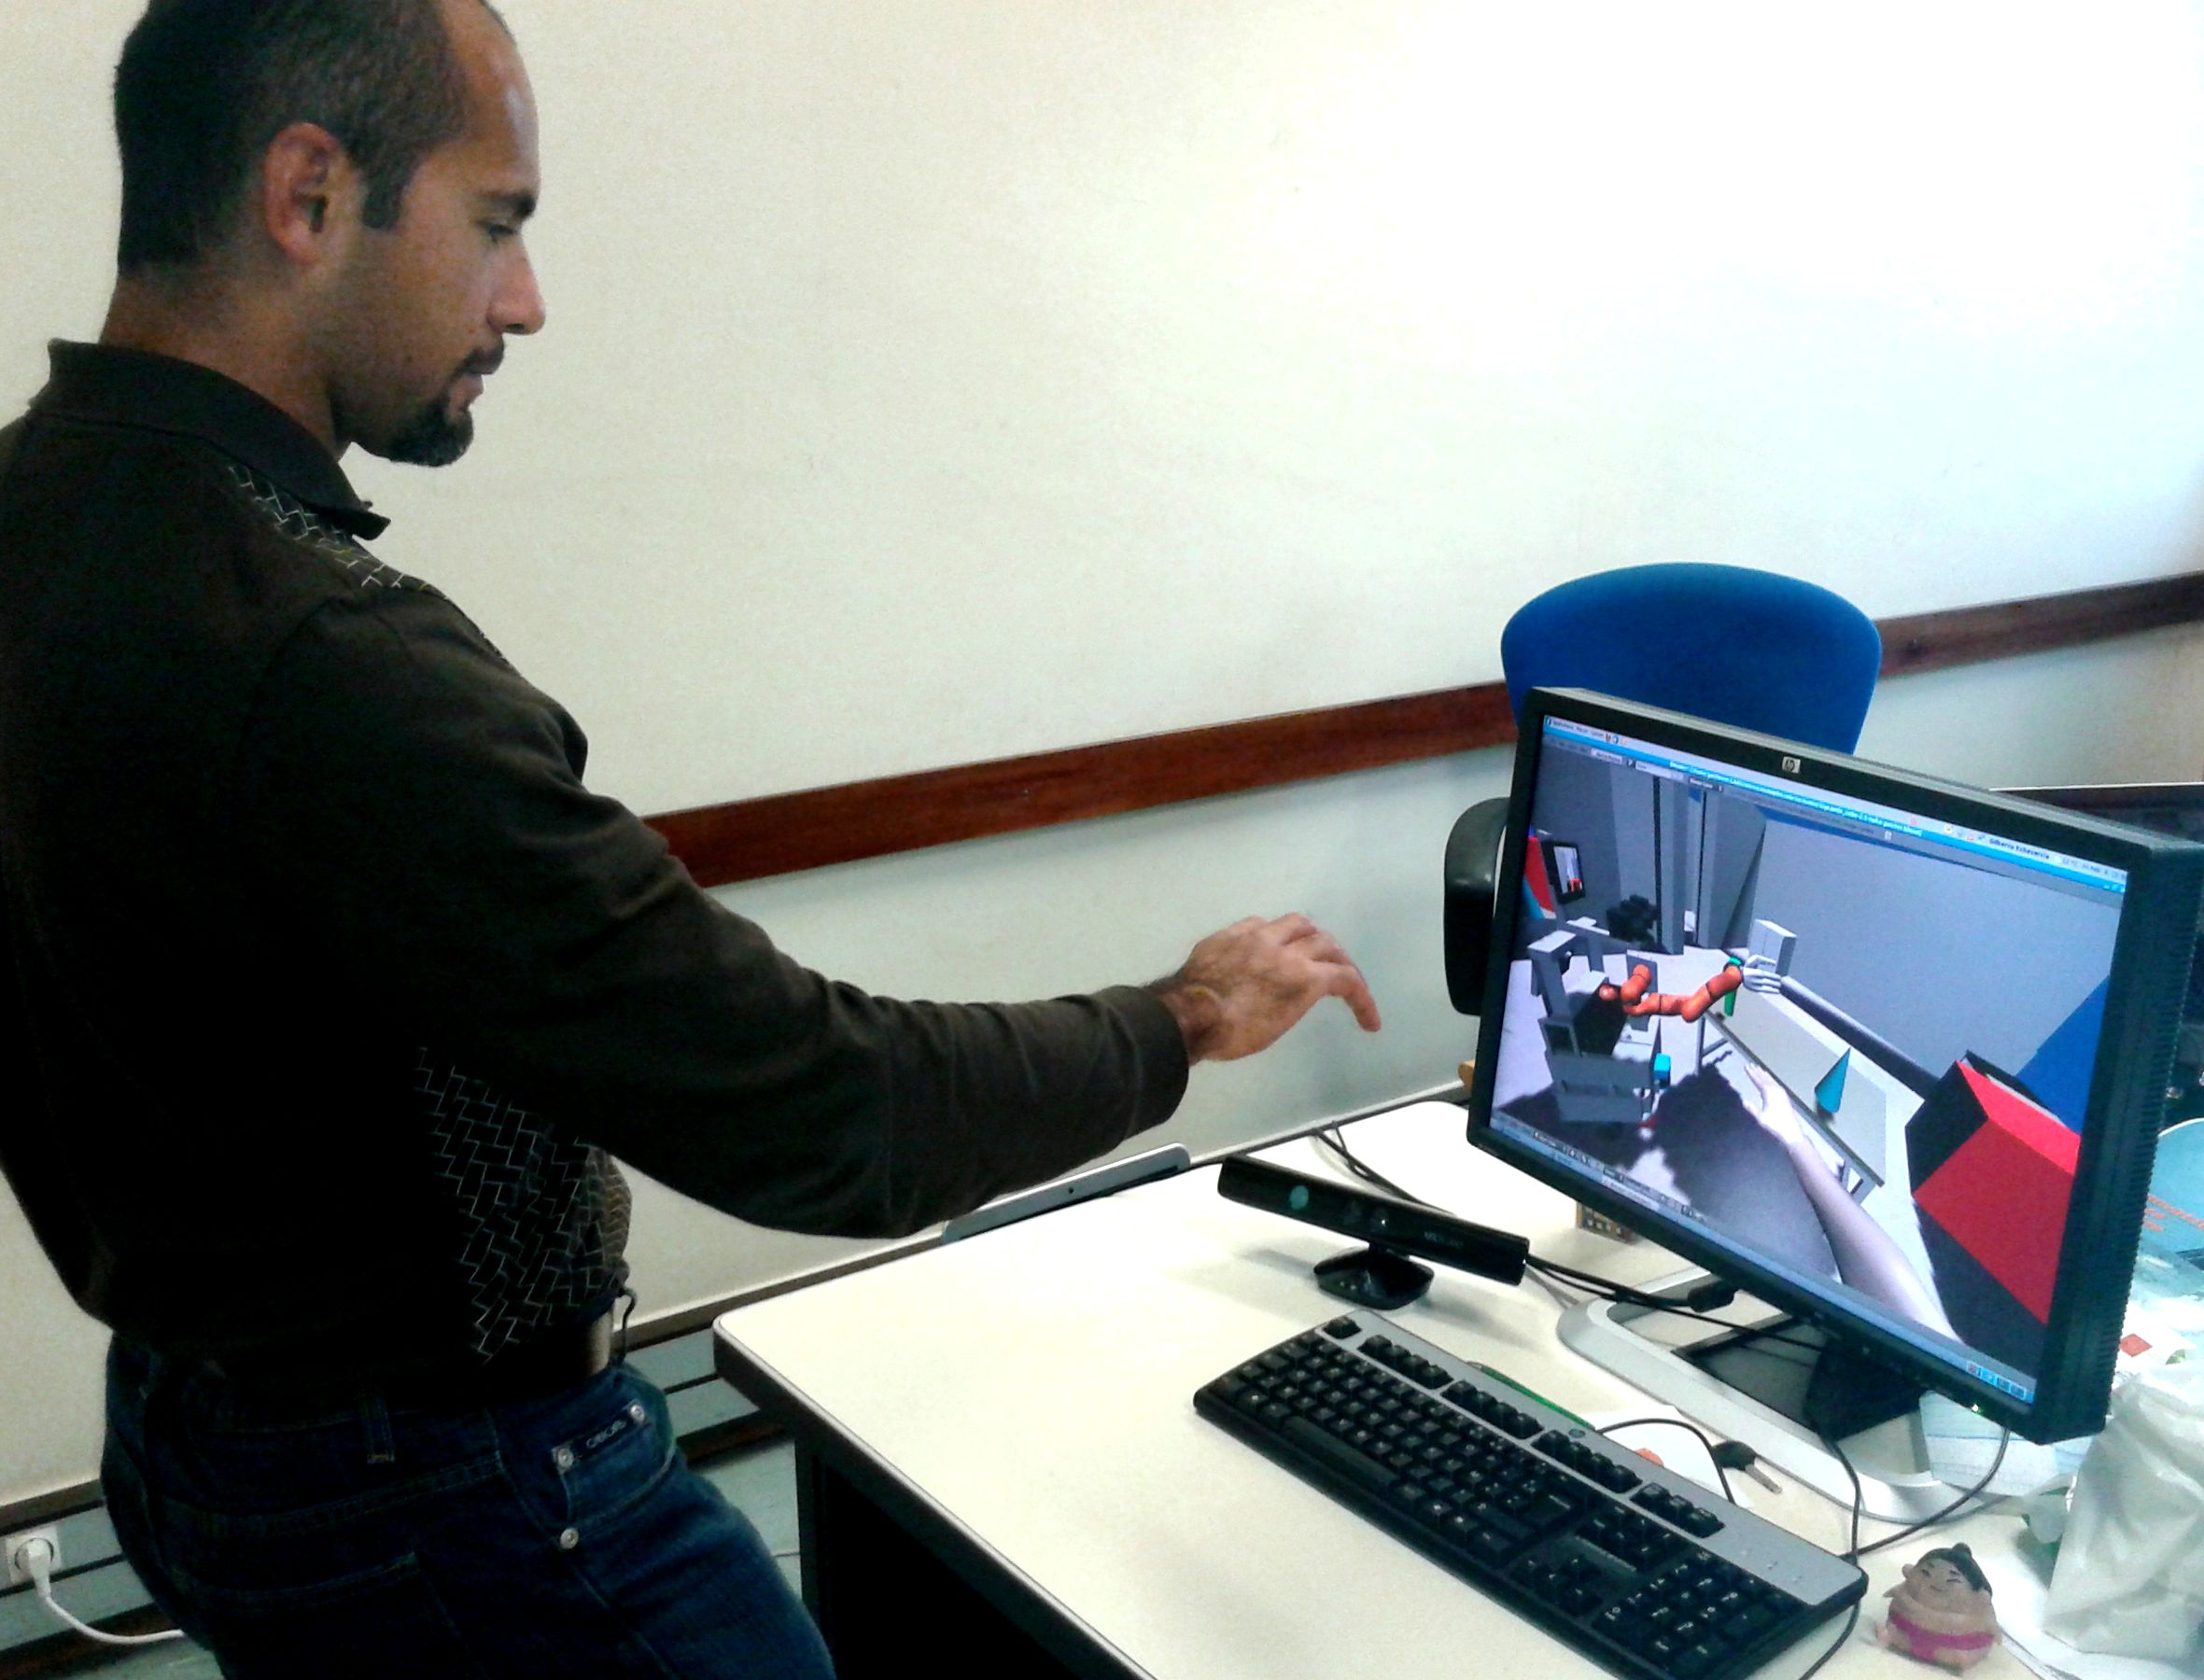
\includegraphics[width=0.7\columnwidth]{experiments/morse-kinect.jpg}
      \caption{The experimental setup with the human avatar controlled from a
      Kinect.}
      \label{fig|kinect-setup}
\end{figure}

An interactive \emph{human avatar} is available in MORSE. It provides a
first-person immersive experience: when started, one can take the role of the
human and control it via the keyboard, a WiiMote or through a Kinect device
(Fig.~\ref{fig|kinect-setup}).

When in first-person mode, the user can interact in several ways with the
environment. He/she can pick and release objects, can open drawers and
cupboards. As any other object, the avatar physically interacts (collision
detection) with the surrounding furnitures.  MORSE exports the position
and posture of the avatar as a global joint state to be used by the real
software components of the robot.

MORSE also offers a special sensor that exports abstracted informations of
objects visible to the robot (called the \emph{semantic camera}). This
sensor typically exports the name, type (glass, table, bottle, etc.), color and
location of objects. Since human-robot interaction often involves
semantic-rich environments, this abstract sensor simplifies the
experiments on such scenarii, by avoiding the added complexity of processing
camera images to detect the objects of interest and exploiting the inherent
knowledge of the simulated world.

\subsubsection{An Experimental Framework}

Due to its nature, MORSE offers two main advantages compared to experiments on
a real robot: light-weight deployment and repeatability. MORSE is already used
for human-robot interaction both at the LAAS-CNRS and at the Technical
University of Munich, Germany.

MORSE is integrated to the LAAS architecture.  In particular, both the human
posture and the object features are integrated with SPARK, a
module dedicated to geometric and temporal reasoning.  This module is a key
component providing a base of facts such as objects' relative placements,
visibility and reachability by the agents present in the scene. It additionally
provides a stable state of the world to the motion planners.

\subsection{Case Studies}
\label{sect|casestudies}

This section reports on three small experiments conducted in the first half of
the PhD. Each of them illustrate one specific aspect of the knowledge base.

The first experiment, \emph{Point \& Learn} shows how the structure
(\emph{TBox}) of the knowledge base can be altered (in this case expanded) at
runtime through pointing interaction.

The second experiment, \emph{Odd One Out} shows how the knowledge model can be
used along with the categorization routines to isolate an ``odd" object, given
a simple context.

Lastly, the third case study is an implementation of the \emph{Spy Game} where
one of the player think of an object and the other one must guess by asking
questions.

It must be noted that these three experiments have been implemented on three
distinct robotic platforms: the \textit{BERT2} robot from the Bristol Robotics
Laboratory (a YARP-based architecture), the \textit{Rosie} robot from the
Technical University of Munich (a ROS-based architecture) and the \textit{Jido}
robot at LAAS-CNRS (based on the LAAS Pocolibs middleware).

\subsubsection{Knowledge acquisition: Point \& Learn}
\label{pointandlearn}

\begin{figure}
\centering

\centering
  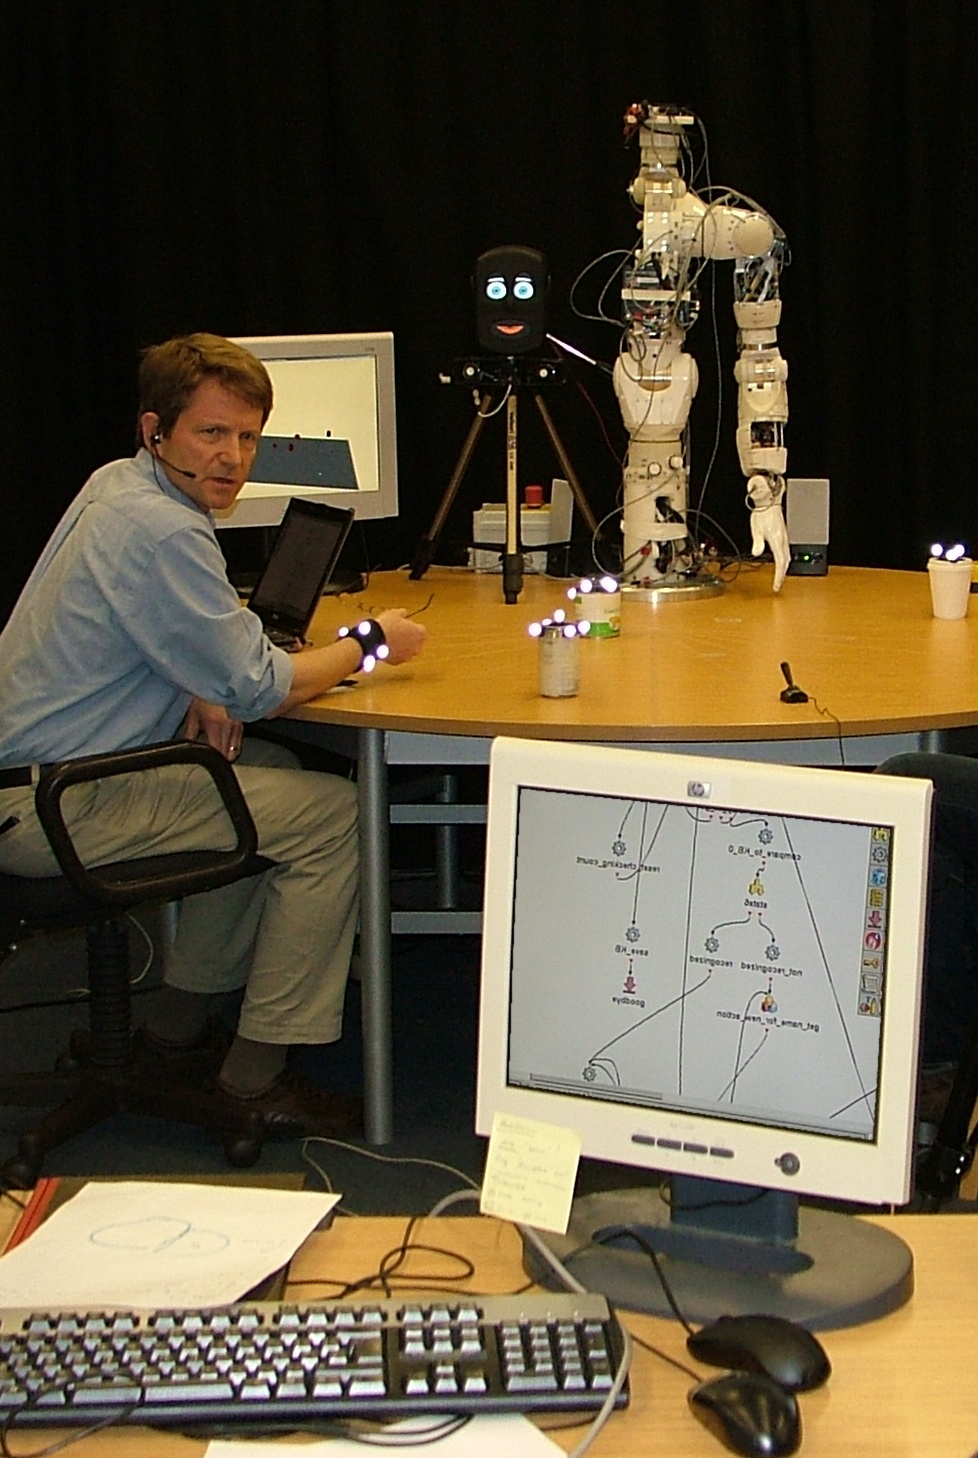
\includegraphics[width=0.4\columnwidth]{experiments/bristol_integration.jpg}
  \caption{Teaching the Bert robot new objects}
  \label{fig|bristol}

\end{figure}

We have implemented a \textit{Point \& learn} behaviour on the Bert robot~\cite{Lallee2010b} (Figure~\ref{fig|bristol}): the user shows an object to the robot, and if the robot sees it for the first time, it will ask for its name and type.

The object perception module relies on motion capture (VICON system) to identify and localize objects. A so-called \textit{primitive detection} module is responsible for updating ORO with the list of objects currently seen by the robot as well as their state (moving or not) and their relations to other objects (touching or not). On the other end, a human-robot interface based on the CLSU Toolkit\footnote{\url{http://cslu.cse.ogi.edu/toolkit/}} is in charge of speech recognition, speech synthesis and basic natural language processing.

By querying ORO for moving objects, the interface retrieves the object ID that has the focus of attention (last moving object), and asks the human for a name and a type if the object is new. Figure~\ref{tab|transcript_bert} reproduces a typical dialog with Bert.

At the end of this sequence, two more RDF statements are added to the robot knowledge base: \texttt{[5001 rdfs:label "coffee-cup"]} and \texttt{[5001 rdf:type Cup]}.

\begin{figure}[!ht]
\centering
	\begin{tabular}{r|p{0.6\columnwidth}}
	\chatN{bert} & Initializing... \textit{[about 5 sec]} ...What's next? \\
	\chatN{human} & \textit{[moves an object]} \\
	\chatN{bert} & \textit{[does not know the object]} How is it called? \\
	\chatN{human} & coffee-cup \\
	\chatN{bert} & Did you say coffee-cup? \\
	\chatN{human} & yes \\
	\chatN{bert} & Ok. Now I know. What kind of object is coffee-cup? \\
	\chatN{human} & a cup \\
	\chatN{bert} & Did you say cup? \\
	\chatN{human} & yes \\
	\chatN{bert} & So coffee cup is a cup. What's next? \\
	\end{tabular}
	\caption{Transcript of a chat with the Bert robot}
	\label{tab|transcript_bert}
\end{figure}

Due to the limitation of the speech recognition software, only a predefined set of names or types could be recognized, thus preventing the robot to add completely original objects.

\subsubsection{Odd One Out}
\label{odd_one_out}

\begin{figure}
\centering

    \subfigure[]{
        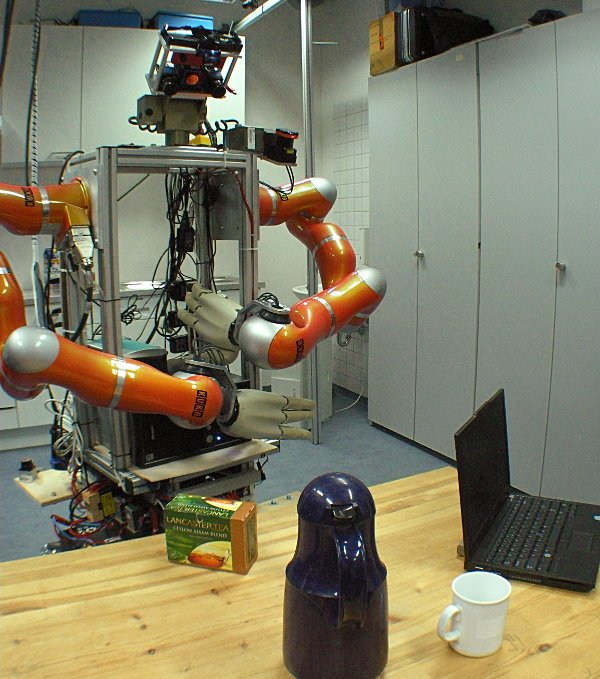
\includegraphics[width=0.4\textwidth]{experiments/kimp1.jpg}
    }
    \subfigure[]{
        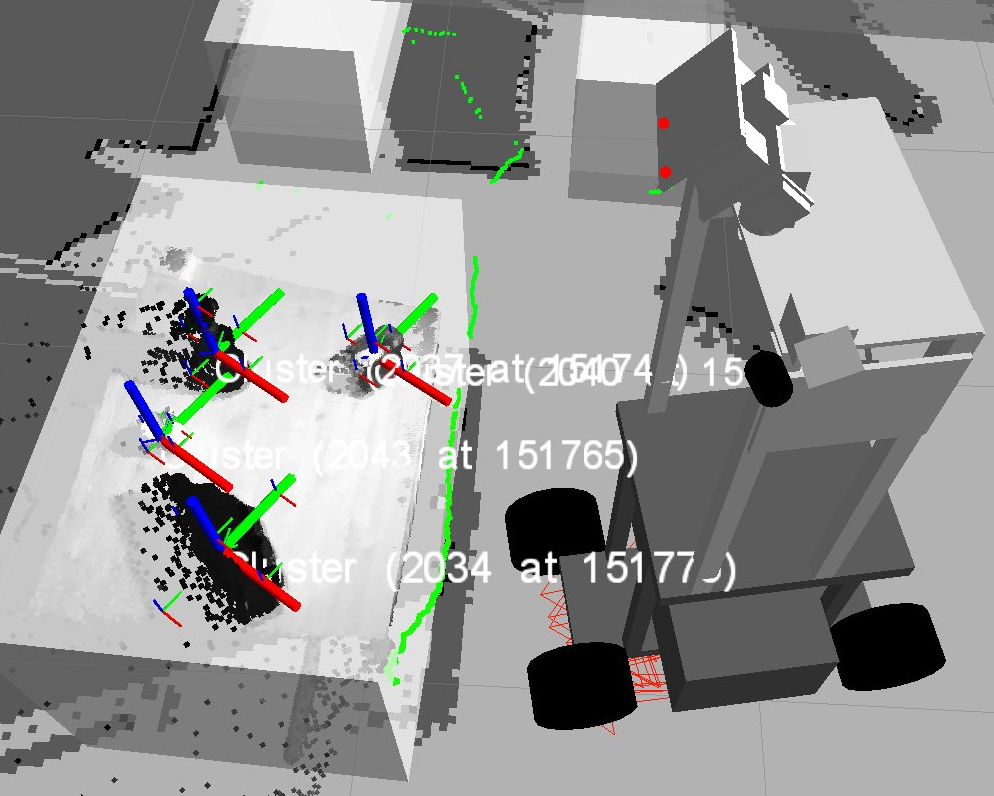
\includegraphics[width=0.4\textwidth]{experiments/rviz.png}
    }
\caption{(a) Rosie, looking for objects it may know, and (b) viewed in RViz. The clusters of point are given an unique identifier by the perception that allow the supervision create the link between the physical objects and their symbolic representation in ORO.}
\label{fig|kimpwatching}
\end{figure}


The \emph{Odd One Out} scenario extends the \textit{Point \& Learn} experiment and completes an on-going experiment at the IAS laboratory where a robot is asked to list missing items on a table being set, based on probabilistic reasoning on previously recorded observations.
%~\cite{Pangercic2009}.

We use ORO to introduce human interactions and common-sense reasoning: the robot picks an unknown object from the table, shows it to the user, and asks about its name and type (Figure~\ref{fig|kimpwatching}). The user continues to describe the object (through concepts) until a concept known by the robot is given. The learning process starts over again with another unknown object. Once all objects are learned, the robot tells which objects do not belong to a typical breakfast table (\textit{i.e.} objects that are neither food or tableware). The human interacts with the robot through a dedicated XMPP bridge, allowing to chat with the robot with a standard Jabber messaging client. Figure~\ref{tab|transcript_kimp} corresponds to a chat session with Rosie.

The supervision (\textsc{cram}\footnote{\textsc{cram} (Cognitive Robotic Abstract Machine) is a RPL-derived framework for rapid development of cognitive robot control programs we currently develop.}~\cite{Beetz2010}) automatically updates the ORO server whenever an object enters or leaves the field of view.
%(the perception is based on the \textsc{CoP} framework~\cite{Klank2009}). 
Therefore, the integration of ORO can be seen as an extension to
the robot's belief state that not only contains abstract identifiers
of the internal object representation used in plans, but also the
semantics and roles of objects in the scenario.

\begin{figure}[!ht]
\centering
	\begin{tabular}{r|p{0.7\columnwidth}}
	\chatN{rosie} & Servus! The Bavarian robot is up and fit! \\
	\chatN{rosie} & What is the name of the WHITE CLUSTER on the TABLE? \\
	\chatN{human} & "Rosie's mug" \emph{[Rosie adds \stmt{OBJ001 rdfs:label "Rosie's mug"} stmt]}\\
	\chatN{rosie} & What kind of object is Rosie's mug? \\
	\chatN{human} & Mug \\
	\chatN{rosie} & What is a Mug? \emph{[Rosie adds \stmt{OBJ001 rdf:type Mug} but it does not know the \emph{Mug} concept]}\\
	\chatN{human} & Tableware \emph{[Rosie knows about \emph{Tableware} - belongs to the common-sense ontology. It adds \stmt{Mug rdfs:subClassOf Tableware}]}\\
	 & (...) \\
	\chatN{rosie} &  What is the name of the BLACK CLUSTER on the TABLE? \\
	\chatN{human} & my laptop \\
	\chatN{rosie} & What kind of object is my laptop? \\
	\chatN{human} & Computer \\
	\chatN{rosie} & What is a Computer? \\
	\chatN{human} & Artifact \\
	\chatN{rosie} & Do you want me to learn more objects? \\
	\chatN{human} & no \\
	\chatN{rosie} & These objects are odd: my laptop \\
	\end{tabular}
	\caption{Transcript of a Jabber session with the robot Rosie. Compared to dialog with Bert (\ref{tab|transcript_bert}), we see here that the robot anchors the new objects in its already acquired knowledge.}
	\label{tab|transcript_kimp}
\end{figure}

By asking in loop the human for the categories of an object until it can connect it to a concept it already knows, the robot accurately anchors perception in its symbolic model and it is able to reason about it. At the end of the experiment, the robot identifies and returns the odd objects for the breakfast table (\textit{i.e.}, in our example, objects that are neither \texttt{Tableware} or \texttt{Food}).

An unexpected example of what the symbolic reasoning layer brings to more traditional robotic architectures emerged during the \emph{Odd One Out} experiment: the perception routines provided segmented blobs corresponding to objects, along with their colours. The supervision would then feed ORO with the visible objects. At some point, ORO suddenly refused to add an object. What seemed at first a communication bug between modules, was actually the consequence of a consistency check by ORO: Because of bad light conditions, the color recognition was not very reliable, and the same object was set to have two different colours at the same time. That was inferred as impossible by ORO and thus discarded. This kind of logical failure can be used to improve low-level perception results by ``closing the loop'' with high-level, symbolic knowledge.


\subsubsection{The Spy game}
\label{spygame}

This game is based on the traditional children game ``I Spy''. The idea is to discover the object or concept one of the participants is thinking of by asking questions such as: ``Is it green? Is it a machine? Is it on your left?'', etc. When playing, children exploit their knowledge about the world while categorizing and describing objects through useful discriminants that allow them to find out the answer as fast as possible while including perspective taking abilities~\cite{Moll2006}.

\begin{figure}
\centering

    \subfigure[]{
        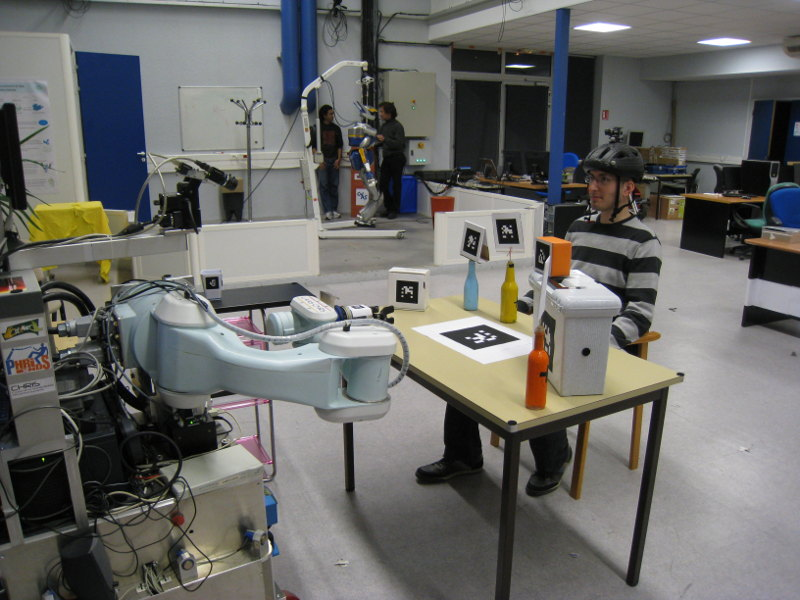
\includegraphics[width=0.4\textwidth]{experiments/spy-game-real.jpg}
    }
    \subfigure[]{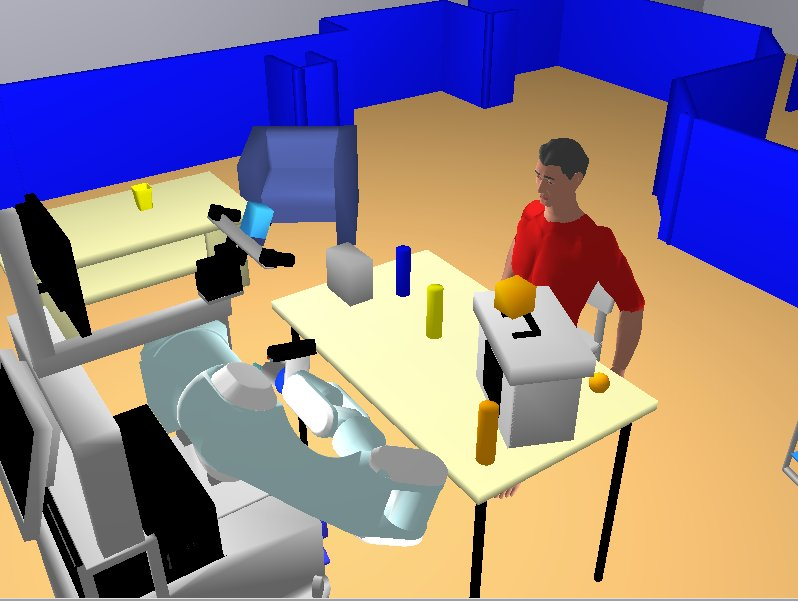
\includegraphics[width=0.4\textwidth]{experiments/spy-game-mhp.jpg}
    }
\caption{Spy game scenario: (a) Real environment and (b) 3D environment model, viewed in \textsc{Move3D}.}
\label{fig|spyGameScenario}
\end{figure}

The scenario for this game (Figure~\ref{fig|spyGameScenario}) consists on a face-to-face interaction where the human thinks of an object present in the environment, while the robot queries the human until either discovering the object or giving up, if no object was found. A categorization example is presented in Figure~\ref{fig|objectsSpyGame}. The game starts with the human user giving a first hint (communication is done through a keyboard and screen), allowing the robot to start the search filtering those objects that fulfill this first description. Based on this subset, ORO provides a descriptor (or set of descriptors) that allows a maximum discrimination among objects in the subset. The robot queries the user about the value of the descriptor (or the most discriminant among the set of descriptors) and with this new information, the current subset of objects is filtered again. The process is repeated until either obtaining a single object that fulfills all the descriptor values, or failing (\textit{i.e.} no object found). 

\begin{figure}[!h]
\centering
\begin{scriptsize}
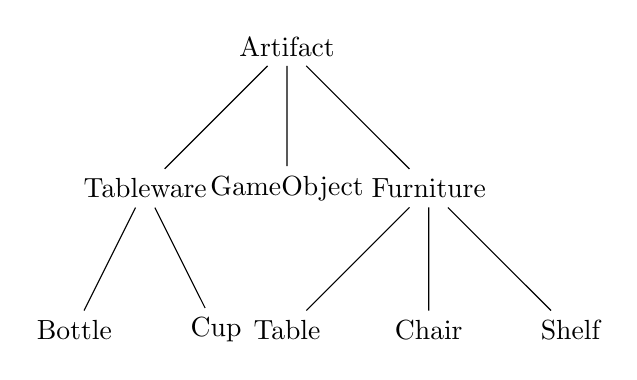
\begin{tikzpicture}[scale=1.2] %[level/.style={sibling distance=30mm/#1},scale=0.8]
	%[edge from parent fork down,
	%every node/.style={fill=black!30,rounded corners},
	%[parent anchor=east,child anchor=west,grow=east,
	%edge from parent/.style={thick,draw}]
	\node {Artifact}
	child {node {Tableware}
		child {node {Bottle}}
		child {node {Cup}}
		}
	child {node {GameObject}}
	child {node {Furniture}
			child {node {Table}}
			child {node {Chair}}
			child {node {Shelf}}};
\end{tikzpicture}
\end{scriptsize}
\caption{Example of object categorization used in the scenario.}
\label{fig|objectsSpyGame}			
\end{figure}

%Thing
%Object
%Tableware
%	- bottle: red, blue, yellow orange
%	- cup: white
%Furniture
%	- table: hrp2table, lowtable
%	- chair: chair1 and chair2
%	- shelf: pink_shelf
%GameObject: spacenavbox, orangebox, accesskit

We have integrated the game in the LAAS-CNRS Jido robot~\cite{Alami1998a}. Objects are identified through a tag-based vision approach\footnote{ARToolKit: \url{http://www.hitl.washington.edu/artoolkit/}} and motion capture is used for human tracking. Their descriptions regarding categories (type of object) and features (color, shape) are manually given in advance. Spatial relationships ({\tt front}, {\tt back}, {\tt left}, etc, and {\tt in}, {\tt on} and {\tt next to}) and visibility (only visible objects for both agents can be considered in the game) are automatically computed on-line by the \textsc{MHP/Move3D} geometric reasoner and planner~\cite{Marin2008}. Figure~\ref{fig|spyGameExample} shows an example of a round game.


\begin{figure}
\centering
	\begin{tabular}{r|p{0.7\columnwidth}}
		\chatN{human} & It is a tableware.\\
		\chatN{jido} & \emph{[retrieves possible objects: blue-bottle, yellow-bottle, orange-bottle, cup-with-handle]} \\
	 			& \emph{[keeps visible objects: blue-bottle, yellow-bottle, cup-with-handle]}\\
				& \emph{[obtains discriminants: type, color.]}\\
				& Which type of object is: bottle or cup? \\
		\chatN{human} & Bottle.\\
		\chatN{jido} & \emph{[obtains possible objects: blue-bottle, yellow-bottle.]}\\
				& \emph{[obtains discriminants: color.]}\\
				& What color the object is: blue or yellow?\\
		\chatN{human} & Blue.\\
		\chatN{jido} & \emph{[obtains possible objects: blue-bottle.]}\\
				& The object is the blue-bottle!	
	\end{tabular}\\
	\caption{Example of the robot playing Spy game.}
	\label{fig|spyGameExample}
\end{figure}

\subsection{First Interaction Experiment}
\label{sect|expe1}

In order to illustrate the approach presented in this paper, we have designed
the following daily life situation. Tom and Jerry are moving to London, so they
are packing things in boxes. The scenario takes places in the living-room,
where Jido (our robot) is observing while they move things here and there. To
assess the reasoning abilities of the robot they ask Jido for information
(entered through keyboard). Ideally, the robot should also perform actions when
required (e.g. hand an object when asking ``give me...''). However, since it is
out of the scope of this work, we do not include any motion from the robot's
side.

Perception of objects is done through a tag-based system and humans are
detected through motion capture. The robot knowledge base is pre-loaded with
the \emph{ORO Commonsense Ontology}\footnote{This ontology can be downloaded
from \url{http://oro.openrobots.org/}.}.  We next describe in detail two
situations where we can follow the internal robot's reasoning and the
interaction with the users.

\subsubsection{Implicit disambiguation through visual perspective taking}

Tom enters the room while carrying a big box (Figure~\ref{fig|vpt}, page 1). He
approaches the table and asks Jido to handle him the video tape: ``Jido, can
you give me the video tape''. The \textsc{Dialogs} module queries the ontology to
identify the object the human is referring to: \stmt{?obj type VideoTape}. 

There are two video tapes in the scene: one on the table, and another one
inside the cardboard box. Thus, the knowledge base returns both: $\Rightarrow$
\concept{?obj = [videoTape1, videoTape2]}. 

However, only one is visible for Tom (the one on the
table). Thus, although there is an ambiguity from the robot's perspective
(since it can see both video tapes), based on the perspective of its human
partner it infers that Tom is referring to the video tape on the table, and not
the one inside the box which is not visible from his view. Therefore,
non-visible objects are removed obtaining: \concept{?obj =[videoTape1]}.

Since only one object is available, the robot infers
that the human refers to it and would eventually execute the command, \ie give
it to the human. Alternatively, the robot could first verify with the human if
that was the object being referred to or not before proceeding to execute the
action. Table~\ref{table|ptbeliefs} lists the robot's beliefs about itself and
its human partner involved in this situation.

\begin{table}
\begin{center}
\begin{tabular}{l}
\hline
Robot's beliefs about itself (\emph{robot's model}):\\
\hline
  \hspace{0.7cm}\stmt{videoTape1 type VideoTape}\\
  \hspace{0.7cm}\stmt{videoTape1 isOn table}\\
  \hspace{0.7cm}\stmt{videoTape1 isVisible true}\\
  \hspace{0.7cm}\stmt{videoTape2 type VideoTape}\\
  \hspace{0.7cm}\stmt{videoTape2 isIn cardBoardBox}\\
  \hspace{0.7cm}\stmt{videoTape2 isVisible true}\\
\hline
\hline
Robot's beliefs about Tom (\emph{Tom's model}):\\
\hline
  \hspace{0.7cm}\stmt{videoTape1 type VideoTape}\\
  \hspace{0.7cm}\stmt{videoTape1 isOn table}\\
  \hspace{0.7cm}\stmt{videoTape1 isVisible true}\\
  \hspace{0.7cm}\stmt{videoTape2 type VideoTape}\\
  \hspace{0.7cm}\stmt{videoTape2 isIn cardBoardBox}\\
  \hspace{0.7cm}\stmt{videoTape2 isVisible false}\\
 \hline
\end{tabular}
\end{center}
\caption{Robot's beliefs about itself and its human partner.}
\label{table|ptbeliefs}
\end{table}

\subsubsection{Explicit disambiguation through verbal interaction and gestures}
\begin{figure}[!ht]
  \centering
  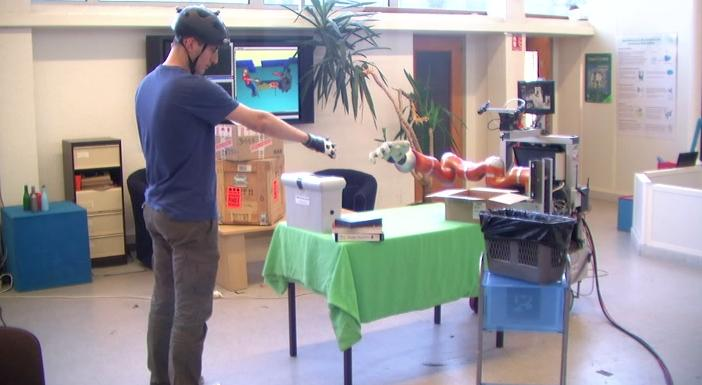
\includegraphics[width=0.9\linewidth]{images/dialogs/inTheBox2.jpg}
\caption{Jerry asks Jido for the content of the box by pointing at it.}
  \label{fig|pointing}
\end{figure}

In this situation, Jerry enters the
living room without knowing where Tom had placed the video tapes. So he first
asks Jido: ``What's in the box?''. Before the robot can answer the question it
has to figure out which box Jerry is talking about. Similar to the previous
situation, there are two available boxes: 

\begin{center}
\begin{tabular}{l}
\stmt{?obj type box}\\
\hspace{0.7cm}$\Rightarrow$ {\tt ?obj = [cardBoardBox, toolbox]}
\end{tabular}
\end{center}

However both are visible and the cognitive ambiguity resolution cannot be
applied. The only option is to ask Jerry which box he is referring to: ``Which
box, the toolbox or the cardboard box?'' Jerry could now simply answer the
question. Instead, he decides to point at it while indicating: ``This box''
(Figure~\ref{fig|pointing}). The robot's perception identifies the {\tt
cardBoardBox} as being pointed at and looked at by the human and updates the
ontology with this new information using a rule available in the commonsense
ontology ({\tt \textbf{pointsAt}(?ag, ?obj) $\land$ \textbf{looksAt}(?ag, ?obj) $\to$
\textbf{focusesOn}(?ag, ?obj)}) The \textsc{Dialogs} module is then able to merge both
sources of information, verbal (``this'') and gestural to distinguish the box
Jerry refers to.

\begin{center}
\begin{tabular}{l}
\stmt{Jerry pointsAt carboardBox}\\
\stmt{Jerry looksAt carboardBox}\\
$\to$ \stmt{Jerry focusesAt carboardBox}\\
\hspace{0.7cm}$\Rightarrow$ {\tt ?obj = [cardBoardBox]}
\end{tabular}
\end{center}

Finally, the \textsc{Dialogs} queries the ontology about the content of the box
and the question can be answered: ``Jido-E''. Note that the object's label is
used instead of its ID. This way we enhance interaction using familiar names
given by the users.

\begin{center}
\begin{tabular}{l}
\stmt{?obj isIn cardBoardBox}\\
\hspace{0.7cm}$\Rightarrow$ \concept{?obj = videoTape2}\\
\end{tabular}
\end{center}

At this point Jerry wants to know where the other tape is, and that is exactly
what he asks Jido: ``And where is the other tape?''. In this occasion, the
\textsc{Dialogs} module is able to interpret that Jerry is not referring to the
video which they were just talking about, but to the other one:

\begin{center}
\begin{tabular}{l}
\stmt{?obj type VideoTape}\\
\stmt{?obj differentFrom videoTape2}\\
\hspace{0.7cm}$\Rightarrow$ \concept{?obj = [videoTape1]}
\end{tabular}
\end{center}

Since there is only one possible ``other'' video (there are only two videos in
the scene), it can directly answer Jerry: ``The other tape is on the table and
next to the toolbox.''

\begin{center}
\begin{tabular}{l}
\stmt{videoTape1 isOn table}\\
\stmt{videoTape1 isNextTo toolbox}
\end{tabular}
\end{center}


\subsection{Second Interaction Experiment}
\label{sect|expe2}

\begin{figure}
    \centering
    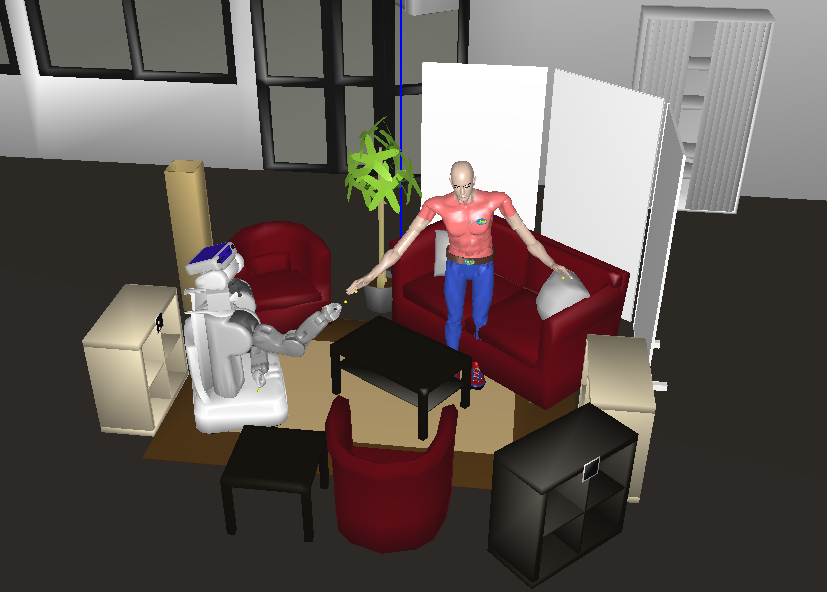
\includegraphics[width=0.7\columnwidth]{experiments/adream-livingroom.png}
    \caption{The ``Living room'' setup}
    \label{fig|livingroom}
\end{figure}


\subsection{Roboscopie}
\label{sect|roboscopie}

\subsubsection{The Performance}

Theatre with robotic actors is an emerging field, with a few previous published
results~\cite{Breazeal2003, Lin2009, Mavridis2009}.

On the 14th of October 2011, we performed for a general public audience (over
300 persons) a 18 min long live theatre play, acted by professional actor
Xavier Brossard and the LAAS/CNRS PR2 robot. The play was created and directed
by Nicolas Darrot, a mixed-media artist from Paris.

The PR2 has been programmed in a 2-months course, re-using several software
components developed at LAAS/CNRS, including the 3D environment for situation
assessment SPARK, the ontology-based knowledge base ORO and the natural-language
processor {\sc Dialogs}.

This video abstract presents the storyline of the play, and underlines some of
the significant outcome for the human-robot interaction community.

The full-length version of the video, along with downloads of the open-source
components, is available from \url{www.laas.fr/roboscopie}.

\begin{figure}
    \centering
    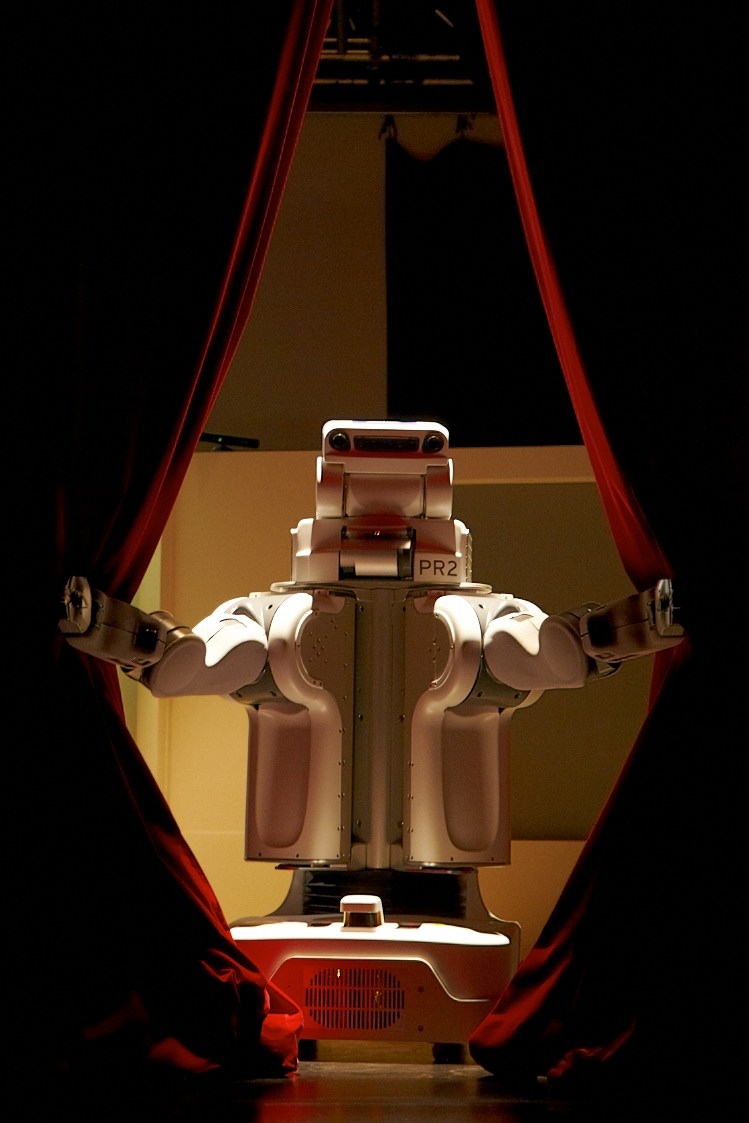
\includegraphics[width=0.5\columnwidth]{experiments/roboscopie.jpg}
    \caption{The PR2 robot at the beginning of the performance.}
    \label{fig|pr2-opens-curtains}
\end{figure}


\subsubsection{Storyline}

The play discusses how humans and robots can find a common ground for understanding
each other, by living in a kind of frontier world, where real objects are replaced 
by abstract, disembodied counterparts.

Xavier and PR2 share a white, almost empty, stage. To get the robot to see his
world, Xavier must keep being recognized by the human tracking module that lies
on the wall, and must stick everywhere 2D barcodes, instead of real
objects. The robot can read and identify these barcodes, and while the stage
gets covered by the tags, the robot constructs for itself a 3D world with the
right-looking objects: a phone, a lamp, a hanger...

While Xavier is drawing by hand more and more of these 2D tags, the robot tries
to offer its help. It brings first a bottle of water, then a fan... which blows
away all Xavier's code. Angry, Xavier leaves, and PR2 remains alone.

The night comes, and the robot decides to explore the stage, scattered with
those barcodes on the ground. On the next morning, Xavier discovers that the
robot's 3D model is a mess, full of random objects: an elephant, a boat, a
van... Xavier resets the robot model and starts to tidy up the place. The robot
decides to help with a trash bin, but suddenly gives up and a new program
starts: a home-training session. Xavier starts the exercises, but as the
program goes along, the robot looks more and more menacing, up to the point
that Xavier shouts "Stop!".

Xavier eventually shows one after the other the objects to the robot,
explaining they are all fake, and like the robot, we realize that everything
was just an experiment.

\subsubsection{Technical overview}

The PR2 robot was running softwares developed at the LAAS/CNRS. While the
performance tries to picture some of the challenges in the human-robot
interaction field, including the needed autonomy of a robot working with
humans, the robot was partially pre-programmed for this theatre performance.

Most of the behaviours were coded in Python, relying both on the PR2 ROS
middleware and on {\sc GenoM}, the LAAS own middleware.

\begin{figure}
    \centering
    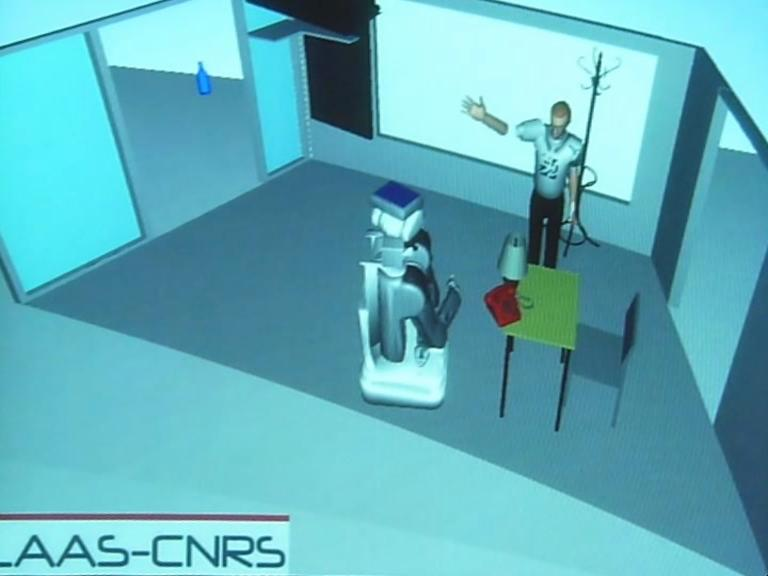
\includegraphics[width=0.8\columnwidth]{experiments/roboscopie-spark.jpg}
    \caption{The robot build a coherent 3D model of its environment through the
    SPARK module}
    \label{fig|spark}
\end{figure}

\paragraph{What was pre-programmed?}

General behaviour: While the real perception routines were running
(see next section), the robot did not have any mean of synchronization with the
human during the play: each sequence was manually started by one of the
engineers.

Places on the stage were hard-coded: for instance, the position of the table
was known to the robot from the beginning, so was the position of the entrance
door, etc.

Postures and manipulation tasks: Manipulation tasks (like grasping
the fan or the paper bin) were much simplified: the robot would simply open its
gripper, and wait for \emph{something} to be detected in its hand. It would
then simply close the gripper. Likewise, the robot special postures to enter or
leave the stage with an object in hand (required to avoid collision with the
door) were all pre-defined.

Speech Understanding: At the end of the play, when Xavier talks to
the robot (\emph{Stop!}, \emph{Look at this phone!}, \emph{Everything is fake},
etc.), sentences were manually typed in the system. We could have used speech
recognition as we do in the laboratory, but converting speech to its textual
version is relatively slow and error prone. So we decided to avoid it on the
stage.

While what Xavier said was actually processed by the robot (see next section),
the actions that followed (like looking at the phone, turning the head back to
the audience,...) were manually triggered.

\paragraph{What was autonomously managed by the robot?}

Navigation: All navigation tasks were computed \emph{live} by
PR2, using the ROS navigation stack. The main script just tells the robot to go
from the engineer desk to the center of the stage for instance. The robot would
then find a path that avoid obstacle.  

Modeling of the environment: The 3D world that is displayed above
the stage during the show (Fig.~\ref{fig|spark}) is a live capture of the
Move3D and SPARK softwares. These softwares are used daily on the robot to
compute trajectories, symbolic locations, visibility and reachability of
objects, etc.

However, during the performance, we deactivated the computation of symbolic
facts (like {\tt xavier looksAt jacket}, {\tt RED\_PHONE isOn table},...) which
is not reliable enough to be used on the stage.

The 2D barcodes are actually a key perception mechanism for our PR2. They are
well identified {\sc ARToolkit} tags used to identify and localize (both for the
position and the orientation) objects surrounding the robot.

Besides, the robot was able to track the human whole-body posture with a
Microsoft Kinect sensor and the {\sc OpenNI} human tracker. In several
occasion, the robot automatically tracks the human head or the human hands with
this system.

Speech Understanding: At the end, Xavier talks to the robot. The
textual version of what he said was fed to the system \emph{as it}. Natural
language understanding is done by the {\tt Dialogs}
module~\cite{Lemaignan2011a} and used extensively the {\tt oro-server} knowledge
database to make sense of the word in the current context. The result of the
language processing was then added back to the knowledge base and automatically
displayed by the {\tt oro-view} OpenGL ontologies viewer.

Hence, the sentence \emph{``look at this phone''} get translated into symbolic
facts: {\tt [human desires action1, action1 type Look, action1 receivedBy
RED\_PHONE]}. The robot is able to know that <this phone> is indeed the {\tt
RED\_PHONE} by taking into account what the human focuses on.

Since the computation of symbolic facts was deactivated, we had to manually add
several symbolic facts in a so-called scenario-specific ontology.

\subsubsection{Significance for HRI}

A first noteworthy achievement of this project from the human-robot
interaction point of view is the use and display of the set of research tools
developed at LAAS in front of a general audience: while the show had been
precisely scripted and rehearsed, the robot was running the same software
components we use on a daily basis in the laboratory.

By building the performance storyline on the current, actual state of robotic
research,  the play also put light on three key questions of today's
human-robot interaction: how the human and the robot can understand each others
(the robot tries to help but remains intrusive)? how to share and coexist in a
common living space? how roles build up between the human and the robot (who
dominates)?


\chapter{Conclusion}
\label{chapter|conclusion}

\section{Discussions}
\label{sect|discussion}

\subsection{Modeling the Real World}
\label{modeling_real_world}

The main challenge we address in this work can be formulated as \emph{How to
model real-world interaction in a symbolic way, processable by the robot to
make decisions}. In the paper we used several times the term \emph{grounding} to
describe the process of binding percepts to symbols (later organized in a
first-order logic framework).  We would like to relate it to
Sloman's~\cite{Sloman2007} stance against the \emph{``Symbol Grounding meme''},
where he argues that symbolic grounding is bound to the representation of
somatic concepts (\ie roughly, the sensori-motor relationships that the robot
learns from its interaction with the world) which in turn severely constraints
the domain of concepts accessible to the robot. We could call this type of
grounding \emph{bottom-up} grounding, and Steels~\cite{Steels2007} claims it is
a solved issue.

For us, \emph{grounding} is on the contrary a \emph{top-down} activity: the
robot needs to automatically bind a representation (for instance, a word
uttered by a human, an image taken from a camera, a sentence extracted from
Wikipedia) to an unambiguous, context-dependent, internal concept. This 
concept may (or may not) be \textit{a priori} available to the robot as a
pre-loaded ontology (what we previously called the cultural background of the
robot).

Note also that perception issues have been solved in our experiments by using a
tag-based object identification method. In
section~\ref{informational_content_extraction} we give an example where the
human says ``the yellow banana is big''. It is assumed in the example that the
robot already knows about a banana instance that is yellow. In our experiments,
this kind of knowledge was either hard coded in scenario-specific ontologies
(\eg \stmt{banana\_01 type Banana} where \concept{banana\_01} is the id of the
banana's tag) or taught to the robot with prescriptive sentences like ``Learn
that this is a banana'' while pointing at the banana's tag. It would be
interesting to extend this approach with automatic classifiers (for colour,
size, etc.). If the robot later discovers a yellowish and large object, an
utterance like ``the yellow banana is big'' could be used to assert that this
object is a banana.  A similar approach focused on the combination of visual
perception and communication modalities to achieve visual learning has been
developed by~\cite{Vrecko2009}.

While the examples we develop are all based on symbols that have a physical
meaning, the system deals equally well with abstract, \emph{exo-somatic},
concepts like \emph{Time}, \emph{Event} or \emph{Place}. Demonstrating this in
real experiments would be an interesting development.

Amongst the other shortcomings of our architecture, neither the \emph{domain of
validity} nor the context of a fact are represented in a satisfying way (we do
store some kind of context --the agent's mental model for instance). This
information is meta-information on the knowledge. While the ORO framework
allows them through \emph{statement reification}, it does not offer yet a
convenient way to store them. One obvious limitation that derives from the lack
of efficient meta-knowledge is the absence of knowledge history.  With ORO, the
robot always lives in the present.

Along the same lines, our current framework lacks a proper management of
uncertainty which is essential for real world environments. A probabilistic
layer should be added by attaching truth probabilities to statements, similar
to~\cite{Jain2009}.

\subsubsection{On Thematic Roles and Action Models}

The current implementation relies on a small, predefined set of action verbs
that can be recognized from natural language
(section~\ref{processing_of_actions}).  This constraint does not come from the
resolution algorithm itself, but rather from the difficulty to automatically
extract the thematic roles associated to a verb.  This could be improved by
linking a symbolic task planner to the \textsc{Dialogs} module to dynamically
provide the list of actions that the robot can process, \ie actions for which
the robot can produce a plan. Additionally, we could exploit on-line resources
like \textsc{VerbNet}~\cite{Kipper2008}, which provides a large
machine-processable lexicon of English verbs along with their thematic roles.

\subsection{Knowledge and Embodiement}

The three experiments that were presented in the paper all illustrate how the
robot makes use of its embodied nature to establish a meaningful communication
with a human. Mainly, because the robot and the human share the same physical
environment and they perceive each other, we are able to create a mutual
context.

Sloman, in~\cite{Sloman2009}, argues however that the strong focus on
embodiment in the robotics community has hindered progress towards natural
human-robot interaction. Our approach has hopefully made clear that, similar to
Beetz et al.~\cite{Beetz2010}, we do not consider embodiment \emph{per se}
outside of a broader symbolic system, \ie our architecture is not bound to the
morphology or the low-level sensori-motor capabilities of a specific agent. 

However, we can build a model of the ``human point of view'' because the robot
perceives the human, and is able to estimate, at least partially, what the
human perceives or not. We infer that a human focuses on some object because
he/she points at it, looks at it, and besides, the object is visible to him.
This relies on the embodied nature of the interaction. In turn, this allows us
to understand the meaning of sentences like ``Give me that''.

We hope that this contribution shows that considering embodiment as the most
challenging and fruitful characteristic of robotics in regards to the whole AI
community does not contradict with a formal, highly symbolic approach of the
representation and decision problems that arise in robotics. 

Let us conclude this article briefly reviewing and linking Roy's list of challenges
for human-robot dialogue with our current approach: 
\begin{itemize}

	\item While more modalities (especially, deictic gestures and social gazes)
	can be added, we have actually proposed a \emph{cross-modal
	representation system}.

	\item One of the main feature of the \textsc{Dialogs} module is its ability
	to interactively ground concepts through disambiguation, bringing the
	ability for the robot to \emph{associate words with perceptual and action
	categories}.

	\item The ORO knowledge base offers some support for the \emph{modeling of
	context}, but a lot remains to be done in this respect.

	\item \emph{Figuring out the right granularity of models} is partially
	solved by supporting both a geometric reasoning level and a purely symbolic
	level. Generally speaking, it appears that complex robotic systems need
	to operate with a dynamic granularity, depending on the task to achieve.

	\item \emph{Temporal modeling} is currently missing in our architecture,
	and symbolic and geometric \emph{planning} is accomplished outside of the
	knowledge representation loop we presented here. We see planning as an
	essential tool to build predictive knowledge, and we are looking into this
	direction.

	\item Since we provide no time management, our system is currently not able
	to \emph{match past (learned) experiences with the current interaction}.
	This ability is obviously a key step for general action recognition, and
	seems of particular importance for the robot to assess the state of the
	interaction with the human.

	\item Finally, Roy mentions \emph{the ability to take into account the
	human perspective}: this is probably our main contribution which we are now
	trying to develop even further towards psychology-inspired experiments.

\end{itemize}


%%%%%%%%%%%%%%%%%%%%%%%%%%%%%%%%%%%%%%%%%%%%%%%%%%%%%%%%%%%%%%%%%%%%%%%%%%%%%%%%%%%%%%%%%%%%
\section{Knowledge-Oriented Architectures}


We have presented qnd illustrated in the preceding chapters how knowledge
streams can be organized within a robotic architecture. Based on the experience
gained while developing and deploying {\sc ORO}, our ontology-based knowledge
server, we have presented how symbolic knowledge could be produced from
perception and geometric reasoning in modules like {\sc SPARK}, a grounded,
perspective-aware, geometric reasoner. We have seen how symbolic knowledge
could be reused by different control systems and task planners like {\sc CRAM},
{\sc SHARY}, {\sc pyRobots}, the {\sc CSLU Toolkit} or {\sc HATP}and how they
take advantage of semantic abstractions provided by knowledge base. We have
also presented the bidirectional integration of {\sc Dialogs}, a natural
language processor for English, with the knowledge base.

Altogether, these components compose an architecture that we call
\emph{knowledge-oriented}:

\begin{itemize}
    
    \item{Knowledge is explicitly stored in one central and consistent
    repository of facts, accessible by all modules.} 

    \item{Knowledge is represented in a strict formalism (OWL statements) and
    with a clearly defined vocabulary (stated in the {\tt
    commonsense.oro.owl} ontology).} 

    \item{The first two points enable both a loosely-coupled architecture where
    modules can very easily be removed or replaced by other ones as long as
    they share the same semantics (modules are defined by the knowledge they
    produce),} 

    \item{and a \emph{symbolic} reactive, event-driven approach to supervision.
    By managing events at the same level as the reasoner, we take full
    advantage of the inference abilities of ORO to trigger events whose
    \texttt{true} conditions can be inferred.} 

    \item{Finally, this architecture allows for the combination of very
    different knowledge modalities in a single homogeneous environment,
    bringing mutual benefits to components. For instance, the dialogue
    processing module can perfectly run without any geometric
    perception, but its disambiguation routines can transparently
    benefit from it when available (since richer symbolic descriptions of
    objects are then available).}

\end{itemize}

This architecture moves away from standard layered approaches. Interactions
between components are mostly bidirectional and, from the software components
point of view, we do not introduce layers of abstraction (we do, however, have
access to the lower level modules of the robot to execute actions, but all
cognition-related modules reside at the same level). This is especially visible
for the dialogue input processing. This component does not simply act as an
alternative perceptual input to the symbolic database, but also actively
queries previously acquired knowledge to disambiguate and validate the newly
created symbolic knowledge.

Our architecture relates but is to be distinguished from \emph{Beliefs,
Desires, Intentions} (BDI) architectures. BDI architectures are primarily
focused on the management of the interaction between knowledge (the beliefs)
and task representation and execution (the desires and the intentions).
\fxfatal{relire rapidement le bouquin sur le multi agent + russell  IA sur BDI
pour pas dire trop de conneries}

This interaction is also central to our approach (as for any cognitive system),
but task representation and task execution is not seen as a monolithic, central
function: it is one of the activity of the robot, split between communication
components (that can acquire desires from interaction agents, amongst other
things), an execution controller that may decide to take an incoming desire
into account, that create its own internal goals, and generate and control
intentions from these goals with the help of a symbolic task planner that has
also direct access to the knowledge base.

But the architecture is not really focused on this workload, and other
activities are conducted without being explicitly considered as desires:
assessment of the situation and the environment, dialogue (including
performative dialogue that can possibly change the internal state of the robot,
but does not lead to the creation of desires,  like question answering or
statement assertion), various background monitoring and recognition tasks, etc.

Regarding the anchoring question, this architecture is bidirectional. The
components we described provide a \textit{bottom-up} grounding process: SPARK
and \textsc{Dialogs} constantly build and push new symbolic contents about the
world to ORO where it becomes accessible to decisional layers. In parallel, ORO
relies on reasoning in a \textit{top-down} way to produce new facts that may
trigger in return physical behaviours. 

We believe that this \emph{knowledge-oriented} approach has a strong potential
not only to enable rich human-robot interaction, but also as a broader approach
to information alignment and fusion in complex robotic systems.  The
versatility of this paradigm could be illustrated by a simple imaginary
scenario with a blind robot and a deaf robot. The blind robot does not see (no
cameras or alike), but someone can verbally describe a scene to it. On the
other hand, the deaf robot has a good vision system, but cannot process verbal
input.  Without any changes to the software architecture that we described,
supervision modules of both robots would be able to perform equally well (to
actually implement this imaginary situation, the blind robot would of course
need \textit{a priori} 3D models of objects talked about to enable planning or
pick and place actions, and the deaf robot would require at least some gesture
interpretation to understand orders).

This architecture may also contribute to bridge the gap between robotics and
psychology: it provides clear entry points to implement some classical
psychology tests to robots. We presented experiments focused on issues related
to perspective taking. By explicitly enabling independent modeling of the
beliefs of each agent, our architecture is especially well suited to set up
cognitive and psychological experiments (such as the \emph{False-Belief}
experiment), which we plan to further explore.


Allen Newell's analysis:
- Knowledge level: deals with language, entailment
- Symbol level: deals with representation, inference


\subsection{Lessons learned from the introduction of a symbolic knowledge layer}

When starting this PhD, we were given \emph{carte blanche} to explore ways to
explicit knowledge in our robot architecture, to make it one of the robot's
resources in its own right.


Knowledge as a observable, quantifiable, measurable, manipulable, palpable resource


Cognitive observability

Allows for both qualitative and quantitative analysis of the beliefs of the robot

Pylyshyn~\cite{Pylyshyn1989} introduces in 1989 the idea of \emph{cognitive
penetrability} in the context of the study of possible strong equivalences
between computational models and the \emph{psychological reality}:

\begin{quote}

    [One of the criterion] relies on the assumption that we can identify
    certain clear cases of phenomenon that should be accounted for at the
    knowledge level, that is, in terms of the representations alone, rather
    than in terms of properties of the cognitive architecture. Phenomena that
    depend in a rational way on subjects' goals, beliefs, and utilities are a
    case in point. For example in psychophysics we assume that if a measure
    (such as a threshold) changes systematically as we change the payoffs (that
    is, the relative cost of errors of commission and of omission), then the
    explanation of that change must be given at the knowledge level -- in terms
    of decision theory -- rather than in terms of properties of sensors or
    other mechanisms that are part of the architecture. In general showing that
    certain empirical phenomena are sensitive to goals and beliefs (or what I
    call \emph{cognitively penetrable}) is prima facie evidence that they
    should not be attributed to properties of the architecture.}

\end{quote}

The introduction of an explicit \emph{knowledge level} in our architecture
makes it possible to effectively assess the cognitive penetrability of the
whole robot behaviours (this is however not new, and traditional BDI
architectures would also make this claim).

Ease modalities merging ('look at this' -> verbal and deictic, 'give me a
banana -> fetch banana picturesfrom the Web...)

Also enables new features: natural language grounding


\subsubsection{Knowledge for interaction}

\subsubsection{Real-World Symbolic Reasoning}

\begin{quote}

    Where to find milk? Milk is a subclass of dairy which is itself a subclass
    of a perishable goods. The usual storage place for perishable goods is the
    fridge, so the milk is likely to be found in a fridge.

\end{quote}

This example of reasoning, quoted from Moritz Tenorth, is a good example of
simple yet non-trivial reasoning. As a matter of fact, very few of such
reasoning cases where positively identified (and consequently implemented as
rules in ORO).

The design choices of our architecture partially explain that fact: first, the
planning task (which is the prototypical reasoning task) is delegated to a
dedicated, external planner. Then, time is not represented in ORO, and
consequently no temporal reasoning takes place at this level: action
recognition or monitoring are handled by other layers, and the underlying
reasoning tasks are not implemented as explicit symbolic rules in the knowledge
base.

The experiments we have conducted are also likely to have too simplistic
semantics to emphasise to let complex reasoning needs to emerge. More
semantically complex scenarii need to be investigated to better stress the
expressiveness and inference abilities provided by description logics.

However, it must also be noted that hundred of trivial (from a human point of
view) inferences (translating inheritance relations, domain/range constraints,
transitivity, etc.) encode a large amount of common-sense knowledge that would
be tedious, to say the least, to manually assert. These trivial inferences are
all the more important that an expressive knowledge representation language is
used: when a language like OWL allows to directly represent concepts like
partitions, cardinality restrictions, properties' ranges and domains, it leads
to a more implicit (because more abstract) description of the vocabulary, that
in turn requires more underlying reasoning. With the progress in the
understanding of the relations between expressiveness and (tractable)
satisfiability, along with the progress of reasoners, more and more of the
inferences do not need to be explicit anymore, and consequently move behind the
scenes.

%%%%%%%%%%%%%%%%%%%%%%%%%%%%%%%%%%%%%%%%%%%%%%%%%%%%%%%%%%%%%%%%%%%%%%%%%%%%%%%%%%%%%%%%%%%%
\section{Towards the next generation of Knowledge Representation Systems for Robotics}
\label{sect|perspectives}


Before writing down the final mark of the thesis, we would like to feed the
reflexion on the future of knowledge and knowledge representation for robots
(service/companion robots in particular, because they are the ones with the
most obvious need of symbolic knowledge for living in complex, interactive,
semantically rich environment, but this also applies to robots in general).

One of the directions that seems both critical and under-studied in our
community is what we can call \emph{context management} in a broad sense.
Managing context means at least two things: recognising contexts and
representing contexts.

Depending on what context we talk about, recognizing contexts can be relatively
easy (who is talking to me? where am I?) to difficult (what past experience
does my interactor implicitly refers to? etc.). One of the main problem we see
with context identification is that it is a fundamentally \emph{multi-scales}
system: at every point, several temporal, spatial, social, cultural context
co-exist and overlap.

This lead to the second aspect, context representation. Techniques for
representation of overlapping pools of knowledge remain to be developed, as
well as efficient algorithms to retrieve (or discard) such context-related
pools of knowledge.

The ability to explicitly manage contexts and context switches would endow the
robot with a cognitive capability similar to what is known as
\emph{context-dependent memory} in cognitive psychology. This is also related to
Tulving's \emph{autonoetic consciousness}~\cite{Tulving1985a}: the ability to
reflect upon its own past or future experiences.

From a technical standpoint, proper context management would mean a transition
from a monolithic knowledge base to an more modular architecture, with either
multiple (overlapping) models or \emph{facets} (one per agent, one per place,
one per period of time, etc.), or maybe a systematic use of reification to
attach to each \emph{atom} of knowledge (the atom is usually the statement. It
could maybe be extended to a small set of cohesive statements) one or several
contexts. The development of modal logic for practical application is also an
important direction to examine.

Much remain to be done to this regards, starting with a formal analysis of what
are the relevant contexts for our robots.

\par

Proper management of inconsistent knowledge is another point that seems of
particular interest. Inconsistencies are mostly considered today as errors
(modeling issues, perception errors, wrong interpretations of communication, etc.)
that prevent at best further reasoning, at worst the use of the knowledge base.

However, from a cognitive point of view, logical inconsistencies are a very
valuable source of knowledge by themselves. We have previously evoked the role
of cognitive dissonances as an intrinsic motivation factor for knowledge
acquisition. This can be generalised to many sources of inconsistencies:
detection of faulty perception and setup of alternative perception strategies,
start of interactions with other agents to fix a wrong model, etc.

Technical handling of inconsistencies also require to better develop
applications of techniques like default logics to robotics.

\par

The systematic study of the relations between symbolic and geometric models are
another large field open to research. While (discrete) symbolic models are
mostly seen as abstractions of a (continuous) geometric model, this link does
not need to be unidirectional. Presupposition accommodation is an example of
{\it a priori} symbolic knowledge that may alter a geometric model. Many more
of these bidirectional relations remain to be identified.

One overlooked aspect of these links between symbolic and geometric realms is
the temporal reasoning resolution: one of the challenging task for a robot
interacting with human relates to action recognition and prediction. While mid-
to longterm action recognition is a well studied field (\cite{Ghallab1996,
Johnson2005, Tenorth2011}, early and fine grained action recognition (like
gesture initiation, back-channel communication -- nodding, social gaze, ... --,
etc.) that are important for smooth interaction, requires geometric reasoning
at relatively high temporal resolution that operates within a symbolic context.
Viewed from a slightly different perspective, better temporal resolution in the
knowledge stack could lead the way to programming paradigms that are both
massively event-oriented and semantically grounded.

\par

And maybe our final point, the knowledge-oriented architectures that are being
build in many robotic research lab around the world have a very specific
characteristic compared to the efforts of other research communities working on
the question of knowledge within systems, be it humans, like in cognitive
psychology, network of computers, like in the semantic web community, or in
other systems: robots are embodied computers. They act and interact in the
physical world, and the physical world plays a key role as a communication
support. At the same time, they are computers, with unlimited access to remote
sources of knowledge via the Web, either as static database, or through
exchanges with other robots.

This dual essence, both as embodied organism and disembodied agent, places the
robot at the crossing of two fundamental approaches to knowledge management:
either physically and experientially grounded, central, internal to the agent,
or on the contrary ungrounded, distributed, pervasive. The robot is currently
the only entity that can merge and take advantage of both. The research efforts
in these directions have started, foundations have been laid (by relying on
standard ontologies to bridge the perception and the symbolic models), much
more remains to be explored.






\printglossaries

\bibliographystyle{ieeetr}
\bibliography{/home/slemaign/work/biblio/biblio_phd_severin}


%%%%%%%%%%%%%%%%%%%%%%%%%%%%%%%%%%%%%%%%%%%%%%%%%%%%%%%%%%%%%%%%%%%%%%%%%%%%%%%%%%%%%%%%%%%%%%%%%%%%%%%

\end{document}


